\documentclass[10pt,mathserif]{beamer}
\usepackage[T5]{fontenc}
\usepackage{fontspec}
\setsansfont{Segoe UI}
%\setmainfont{Segoe UI}
\usepackage[utf8]{inputenc}
% Style
\usepackage{graphicx,amsmath,amssymb,tikz,psfrag,amsthm,enumerate}
\usepackage[backend=biber,style=numeric,citestyle=ieee]{biblatex}
%\usepackage[backend=biber,style=authoryear,citestyle=ieee]{biblatex}

\addbibresource{references.bib}

% ~~~~~~~~~~~
% References
%\addbibresource{references.bib}


%********************* Custom  *********************  

% ~~~~~~~~~~~~ Custom ~~~~~~~~~~~~
%\usepackage{framed}
\usepackage[capitalise]{cleveref}
\usepackage{algorithm,algorithmicx,algpseudocode}
\usepackage{array}
\usepackage[parfill]{parskip}
\usepackage{caption}
\captionsetup[figure]{labelformat=empty}
%\usepackage{subcaption}
\usepackage{bm}
 \usepackage{amsfonts,amscd}
\usepackage{gensymb}
\usepackage[]{units}
\usepackage{listings}
\usepackage{multicol}
\usepackage{tcolorbox}
% -- \usepackage{physics}
\usepackage{ulem}
% ~~~~~~~~~~~~ Custom ~~~~~~~~~~~~
\graphicspath{{images/}}
\usepackage{hyperref}

% ~~~~~~~~~~~ Default ~~~~~~~~~~~
\newcommand{\ones}{\mathbf 1}
\newcommand{\reals}{{\mbox{\bf R}}}
\newcommand{\integers}{{\mbox{\bf Z}}}
\newcommand{\symm}{{\mbox{\bf S}}}  % symmetric matrices

\newcommand{\nullspace}{{\mathcal N}}
\newcommand{\range}{{\mathcal R}}
\newcommand{\Rank}{\mathop{\bf Rank}}
\newcommand{\Tr}{\mathop{\bf Tr}}
\newcommand{\diag}{\mathop{\bf diag}}
\newcommand{\card}{\mathop{\bf card}}
\newcommand{\rank}{\mathop{\bf rank}}
\newcommand{\conv}{\mathop{\bf conv}}
\newcommand{\prox}{\mathbf{prox}}

\newcommand{\Expect}{\mathop{\bf E{}}}
\newcommand{\Prob}{\mathop{\bf Prob}}
\newcommand{\Co}{{\mathop {\bf Co}}} % convex hull
\newcommand{\dist}{\mathop{\bf dist{}}}
\newcommand{\argmin}{\mathop{\rm argmin}}
\newcommand{\argmax}{\mathop{\rm argmax}}
\newcommand{\epi}{\mathop{\bf epi}} % epigraph
\newcommand{\Vol}{\mathop{\bf vol}}
\newcommand{\dom}{\mathop{\bf dom}} % domain
\newcommand{\intr}{\mathop{\bf int}}
\newcommand{\sign}{\mathop{\bf sign}}

\newcommand{\cf}{{\it cf.}}
\newcommand{\eg}{{\it e.g.}}
\newcommand{\ie}{{\it i.e.}}
\newcommand{\etc}{{\it etc.}}


% ~~~~~~~~~~~ Custom ~~~~~~~~~~~
%new commands
\newcommand{\der}[2]{\frac{d#1}{d#2}}
\newcommand{\nder}[3]{\frac{d^#1 #2}{d #3 ^ #1}}
\newcommand{\pder}[2]{\frac{\partial #1}{\partial #2}}
\newcommand{\npder}[3]{\frac{\partial ^#1 #2}{\partial #3^#1}}
\newcommand{\sentencelist}{def}
\newcommand{\overbar}[1]{\mkern 1.5mu\overline{\mkern-1.5mu#1\mkern-1.5mu}\mkern 1.5mu}
\newcommand{\lined}{\overbar}
\newcommand{\perm}[2]{{}^{#1}\!P_{#2}}
\newcommand{\comb}[2]{{}^{#1}C_{#2}}
\newcommand{\intall}{\int_{-\infty}^{\infty}}
\newcommand{\Var}[1]{\text{Var}\left(#1\right)}
\newcommand{\E}[1]{\text{E}\left(#1\right)}
\newcommand{\define}{\equiv}
\newcommand{\diff}[1]{\mathrm{d}#1}
\newcommand{\empy}[1]{{\color{darkorange}\emph{#1}}}
\newcommand{\empr}[1]{{\color{cardinalred}\emph{#1}}}

%********************* Custom ********************* 
\newcommand{\vardbtilde}[1]{\tilde{\raisebox{0pt}[0.85\height]{$\tilde{#1}$}}}
\newcommand{\defeq}{\coloneqq}
\newcommand{\grad}{\nabla}
%\newcommand{\E}{\mathbb{E}}
%\newcommand{\Var}{\mathrm{Var}}
\newcommand{\Cov}{\mathrm{Cov}}
\newcommand{\Ea}[1]{\E\left[#1\right]}
\newcommand{\Eb}[2]{\E_{#1}\!\left[#2\right]}
\newcommand{\Vara}[1]{\Var\left[#1\right]}
\newcommand{\Varb}[2]{\Var_{#1}\left[#2\right]}
\newcommand{\kl}[2]{D_{\mathrm{KL}}\!\left(#1 ~ \| ~ #2\right)}
\newcommand{\pdata}{{p_\mathrm{data}}}
\newcommand{\bA}{\mathbf{A}}
\newcommand{\bI}{\mathbf{I}}
\newcommand{\bJ}{\mathbf{J}}
\newcommand{\bH}{\mathbf{H}}
\newcommand{\bL}{\mathbf{L}}
\newcommand{\bM}{\mathbf{M}}
\newcommand{\bQ}{\mathbf{Q}}
\newcommand{\bR}{\mathbf{R}}
\newcommand{\bzero}{\mathbf{0}}
\newcommand{\bone}{\mathbf{1}}
\newcommand{\bb}{\mathbf{b}}
\newcommand{\bu}{\mathbf{u}}
\newcommand{\bv}{\mathbf{v}}
\newcommand{\bw}{\mathbf{w}}
\newcommand{\bx}{\mathbf{x}}
\newcommand{\by}{\mathbf{y}}
\newcommand{\bz}{\mathbf{z}}
\newcommand{\bxh}{\hat{\mathbf{x}}}
\newcommand{\btheta}{{\boldsymbol{\theta}}}
\newcommand{\bphi}{{\boldsymbol{\phi}}}
\newcommand{\bepsilon}{{\boldsymbol{\epsilon}}}
\newcommand{\bmu}{{\boldsymbol{\mu}}}
\newcommand{\bnu}{{\boldsymbol{\nu}}}
\newcommand{\bSigma}{{\boldsymbol{\Sigma}}}



%
% Đổi tên mặc định
\renewcommand{\chaptername}{Chương}
\renewcommand{\figurename}{Hình}
\renewcommand{\tablename}{Bảng}
\renewcommand{\contentsname}{Mục lục}
\renewcommand{\listfigurename}{Danh sách hình}
\renewcommand{\listtablename}{Danh sách bảng}
\renewcommand{\appendixname}{Phụ lục}
% Định nghĩa
\newtheorem{definition}{Định nghĩa}


\renewcommand{\figureautorefname}{Hình}
% \renewcommand{\thesection}{\arabic{section}}
% \renewcommand\thesubsection{\alph{subsection}.}
\renewcommand{\thefigure}{\arabic{figure}}
\renewcommand{\theequation}{\arabic{equation}} % Change equation numbering style to consecutive numbers
\renewcommand{\equationautorefname}{Phương trình} % Change "Equation" to "Formula"

\newcommand*\concat{\mathbin{\|}} % parallel




\lstdefinestyle{mystyle}{
	    backgroundcolor=\color{backcolour},   
	    commentstyle=\color{codegreen},
	    keywordstyle=\color{magenta},
	    numberstyle=\tiny\color{codegray},
	    stringstyle=\color{codepurple},
	    basicstyle=\footnotesize,
	    breakatwhitespace=false,     
	    breaklines=true,                 
	    captionpos=b,                    
	    keepspaces=true,                 
	    numbers=left,                    
	    numbersep=5pt,                  
	    showspaces=false,                
	    showstringspaces=false,
	    showtabs=false,                  
	    tabsize=2
	}
\lstset{style=mystyle}




\definecolor{codegreen}{rgb}{0,0.6,0}
\definecolor{codegray}{rgb}{0.5,0.5,0.5}
\definecolor{codepurple}{rgb}{0.58,0,0.82}
\definecolor{backcolour}{rgb}{0.95,0.95,0.92}

% \logo{
\includegraphics[height=0.6cm]{hcmus}}
% ~~~~~~~~~~~~ Custom ~~~~~~~~~~~~

%% formatting
\mode<presentation>
{
\usetheme{default}
%\usetheme{Berlin}
%\usetheme{Stanford}
\useinnertheme{circles}
}
\setbeamertemplate{navigation symbols}{}
\usecolortheme[rgb={0.13,0.28,0.59}]{structure}
%\setbeamertemplate{itemize subitem}{--}
\setbeamertemplate{frametitle} {
	\begin{center}
	  {\large\bf \insertframetitle}
	\end{center}
}

\newcommand\footlineon{
  \setbeamertemplate{footline} {
    \begin{beamercolorbox}[ht=2.5ex,dp=1.125ex,leftskip=.8cm,rightskip=.6cm]{structure}
      \footnotesize \insertsection
      \hfill
      {\insertframenumber}
    \end{beamercolorbox}
    \vskip 0.45cm	
  }
}
\footlineon

\AtBeginSection[] 
{ 
	\begin{frame}<beamer> 
		\frametitle{Outline} 
		\tableofcontents[currentsection,currentsubsection] 
	\end{frame} 
} 

\title{\large \bfseries OpenHuman: Sinh cử chỉ dựa trên âm thanh}
\subtitle{The synthesis system for conversational gestures based on emotion and semantics}

\author{Thanh Hoang-Minh \\ [2ex]
	Giảng viên hướng dẫn: \\ PGS. TS. Lý Quốc Ngọc}
%	\footnotesize \href{mailto:hmthanhgm@gmail.com}{(MSSV: 21C11029)}}

\institute{
	
\includegraphics[height=2cm]{hcmus.png}\\
	Faculty of Information Technology\\
	VNUHCM-University of Science}
\date{\today}

% ~~~~~~~~~~~~~~~~~~~~~~~~~~~~~~~~~~~~~~~~
\begin{document}

%\begin{frame}[plain]
%	\titlepage
%\end{frame}


%\section{Minh hoạ}

\begin{frame}{Minh họa quá trình sinh cử chỉ}
	\vspace{10pt}
	\begin{columns}
		\begin{column}{0.7\textwidth}
			\begin{itemize}
				\item Sinh cử chỉ (Gesture Generation) là gì?
				
				\begin{figure}[h]
					\centering
					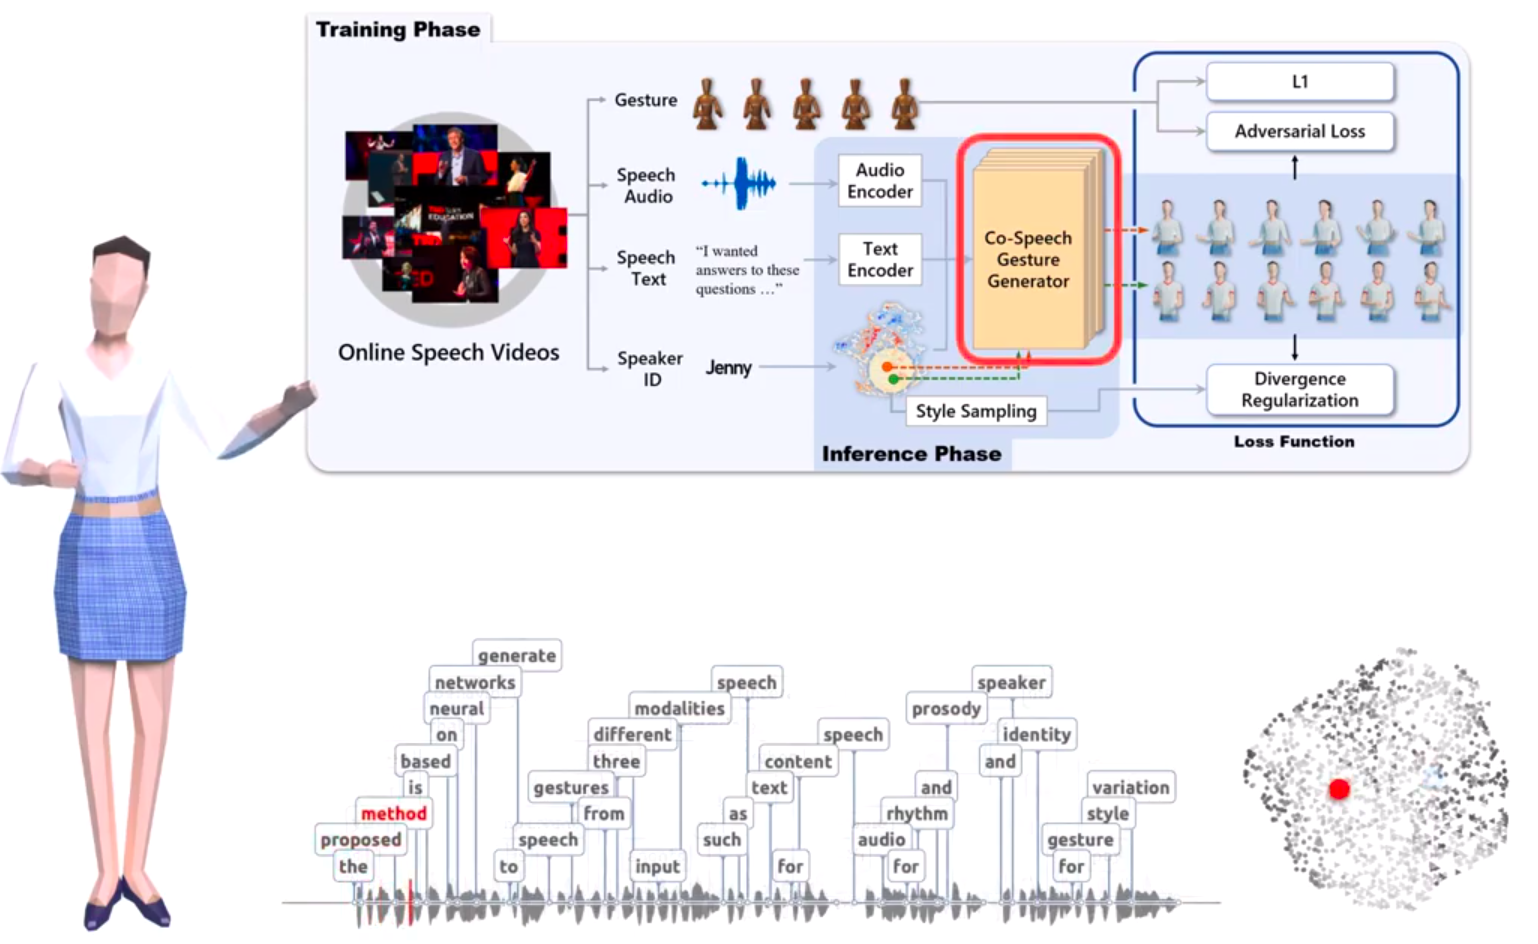
\includegraphics[width=\textwidth]{GestureGenerationExplain}
				\end{figure}
			
%				\item Mục tiêu của việc sinh cử chỉ?
%					\begin{quote}
%					"The goal of Gesture Generation is to generate gestures that are natural, realistic, and appropriate for the given context."
%				\end{quote}
			\end{itemize}
			ACM CCS: • Human-centered computing → Human computer interaction (HCI).
			
		\end{column}
		\begin{column}{0.3\textwidth} % Right column for image
			\begin{figure}[h]
			\centering
			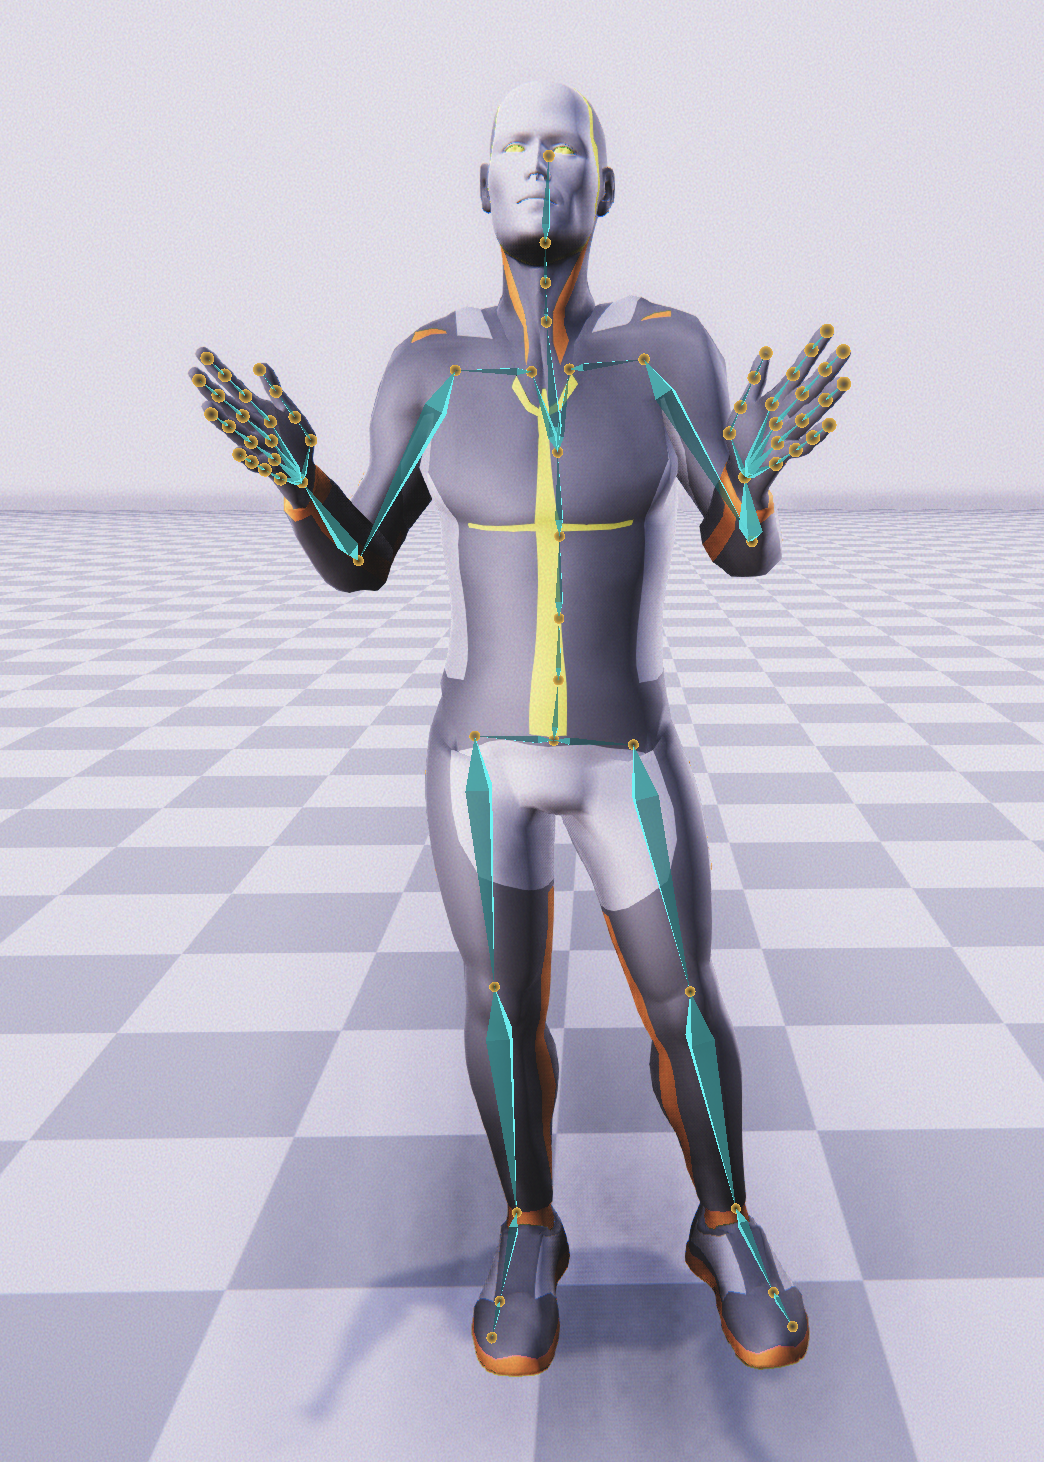
\includegraphics[height={6cm}]{SampleAnimation}
			
%				\begin{quote}
%					{\tiny
%					"Your work is gonna fill a large part of your life . And the only way to be truly satisfied is to do what you believe is great work and the only way to do great work is to love what you do."}
%				\end{quote}
				
			{
			\small Demo Gesture Generation: \href{https://www.youtube.com/watch?v=B6nv1kQmi-Q}{\textcolor{blue}{\uline{Youtube}}}
			}
			\end{figure}
		\end{column}
	\end{columns}
\end{frame}

%\begin{frame}
%\frametitle{Bulleted list}
%\begin{itemize}\itemsep=12pt
%\item XXX
%\vspace*{0.5em}
%\begin{itemize}
%\item XXX
%\item XXX
%\item XXX
%\end{itemize}
%\item XXX
%\vspace*{0.5em}
%\begin{itemize}
%\item XXX
%\item XXX
%\item XXX
%\end{itemize}
%\item XXX
%\end{itemize}
%\end{frame}

%\begin{frame}
%\frametitle{Pictures with tikz}
%\begin{center}
%\begin{tikzpicture}
%	[scale=1.5,dot/.style={circle,draw=black!100,fill=black!100,thick,inner sep=0pt,minimum size=2pt}]
%    \node[dot] at (-1,0) (n1) {};
%    \node[dot] at (0,1)  (n2) {};
%    \node[dot] at (1,0)  (n3) {};
%    \node[dot] at (0,-1) (n4) {};
%    \draw[gray] (-1.5,0) -- (1.5,0);
%    \draw[gray] (0,-1.5) -- (0,1.5);
%    \draw[black,thick] (n1) -- (n2) -- (n3) -- (n4) -- (n1) -- cycle;
%    \draw[orange,thick] (-1,0.5) -- (0,1) -- (1,1.5);
%\end{tikzpicture}
%\qquad
%\begin{tikzpicture}
%	[scale=1.5,dot/.style={circle,draw=black!100,fill=black!100,thick,inner sep=0pt,minimum size=2pt}]
%    \draw[gray] (-1.5,0) -- (1.5,0);
%    \draw[gray] (0,-1.5) -- (0,1.5);
%    \draw[black,thick] (-1,1) -- (0,0) -- (1,1);
%\end{tikzpicture}
%\end{center}
%\end{frame}


%\begin{frame}
%\frametitle{Pictures with tikz}
%\begin{itemize}\itemsep=12pt
%	\item convex envelope of (nonconvex) $f$ is the largest convex underestimator $g$
%    \item \ie, the best convex lower bound to a function
%        \vspace*{1em}
%\begin{center}
%\begin{tikzpicture}
%    \draw[gray] (-1.5,0) -- (1.5,0);
%    \draw[gray] (0,-0.5) -- (0,1.5);
%    \draw[black,thick] (-1,1) -- (0,0) -- (0.5,0.5) -- (1,-0.25) -- (2,1);
%    \draw[black,dashed] (0,0) -- (1,-0.25);
%\end{tikzpicture}
%\end{center}
%%    \item \textbf{example}: $\ell_1$ is the envelope of $\card$ (on unit $\ell_\infty$ ball)
%%    \item \textbf{example}: $\|\cdot\|_*$ is the envelope of $\rank$ (on unit spectral norm ball)
%%    \item various characterizations: \eg, $f^{**}$ or convex hull of epigraph
%\end{itemize}
%\end{frame}

%\section{Giới thiệu}

\begin{frame}{Động lực nghiên cứu}
	\vspace{5pt}
	
	\begin{columns}
	% Left column
	\begin{column}{0.7\textwidth}
		\textbf{Text-base Deep Learning}
		\begin{itemize}
			\item ChatGPT, Alexa, Character.AI,..
			\item Text to speech, text to text,..
		\end{itemize}
		
		\textbf{Text/audio to Realistic Digital Humam}
		
		\begin{itemize}
			\item Video-base (HeyGen, Midjourney,...)
			\item Rendering-base:
			\begin{itemize}
				\item Character model (Gaussian Splatting)
				\item Character animation: (3D keypoints)
			\end{itemize}
		\end{itemize}
		\vspace{5pt}
		\centering
		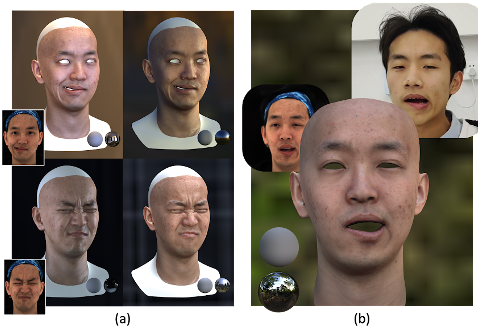
\includegraphics[width=0.8\textwidth]{FacialAsset.png}
	\end{column}
	
	% Right column
	\begin{column}{0.3\textwidth}
		\begin{figure}
				
\includegraphics[width=\textwidth]{UniversalHuman.png}
%				\caption{\small Minh hoạ người kỹ thuật số siêu thật (realistic digital human)}
		\end{figure}
		
		\begin{figure}
			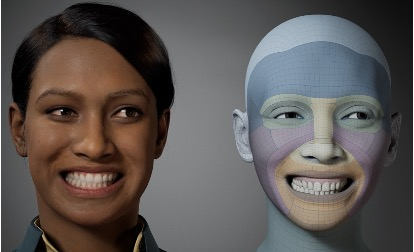
\includegraphics[width=\textwidth]{MetaHuman.jpg}
			\caption{\small Minh hoạ người kỹ thuật số siêu thật (realistic digital human)}
		\end{figure}
	
	\end{column}
	
	\end{columns}
\end{frame}

\begin{frame}
	\begin{columns}
		\begin{column}{0.6\textwidth}
			\centering
			{\Large
			$\{ \mathbf{b}_1, \cdots \mathbf{b}_{75} \}$}
			\vspace{10pt}
			
			\begin{figure}[H]
				\centering
				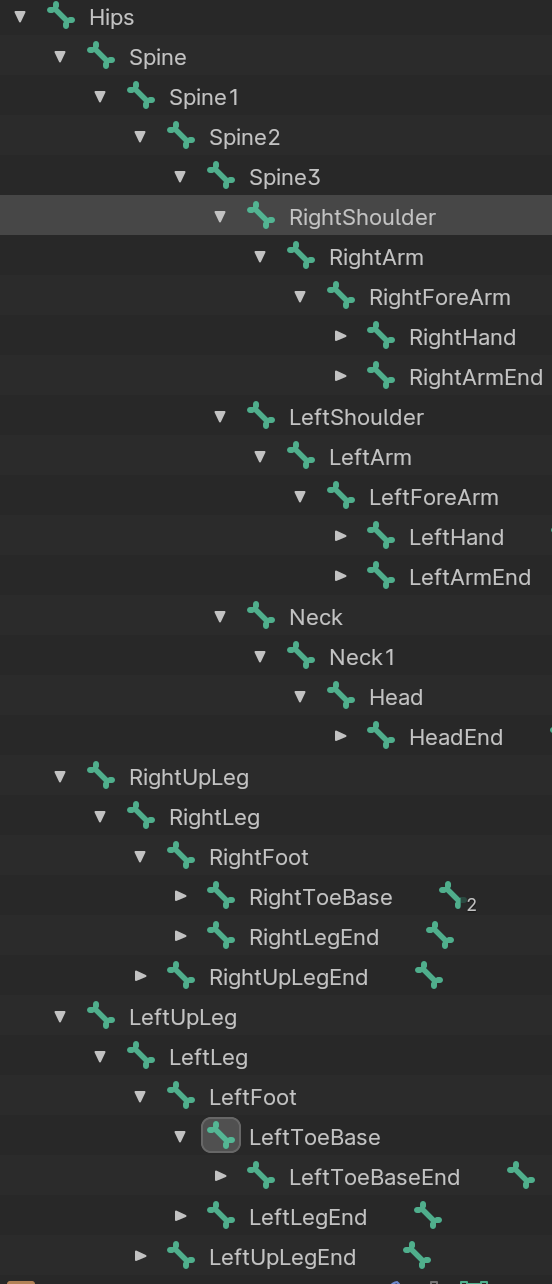
\includegraphics[width=.5\textwidth]{Bone}
			\end{figure}
			
			\vspace{10pt}
			{\Large
				$\mathbf{b}_{i} = \{p_x, p_y, p_z, r_x, r_y, r_z\}$}
		\end{column}
		
		\begin{column}{0.4\textwidth}
			\begin{figure}[h]
				\centering
				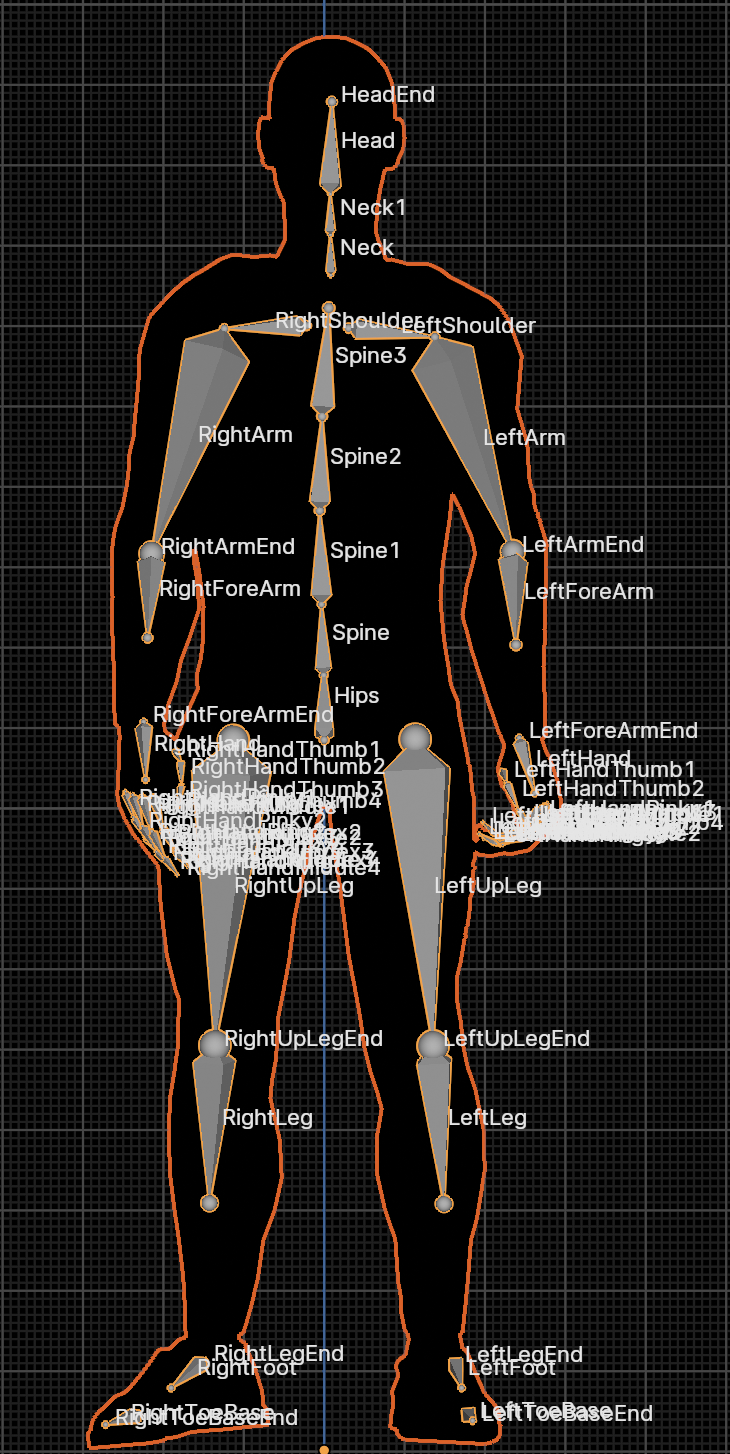
\includegraphics[width=\textwidth]{Skeleton}
			\end{figure}
		\end{column}
		
	\end{columns}
	
\end{frame}

%Dữ liệu cử chỉ cần học
\begin{frame}
		\begin{figure}[h]
		\centering
		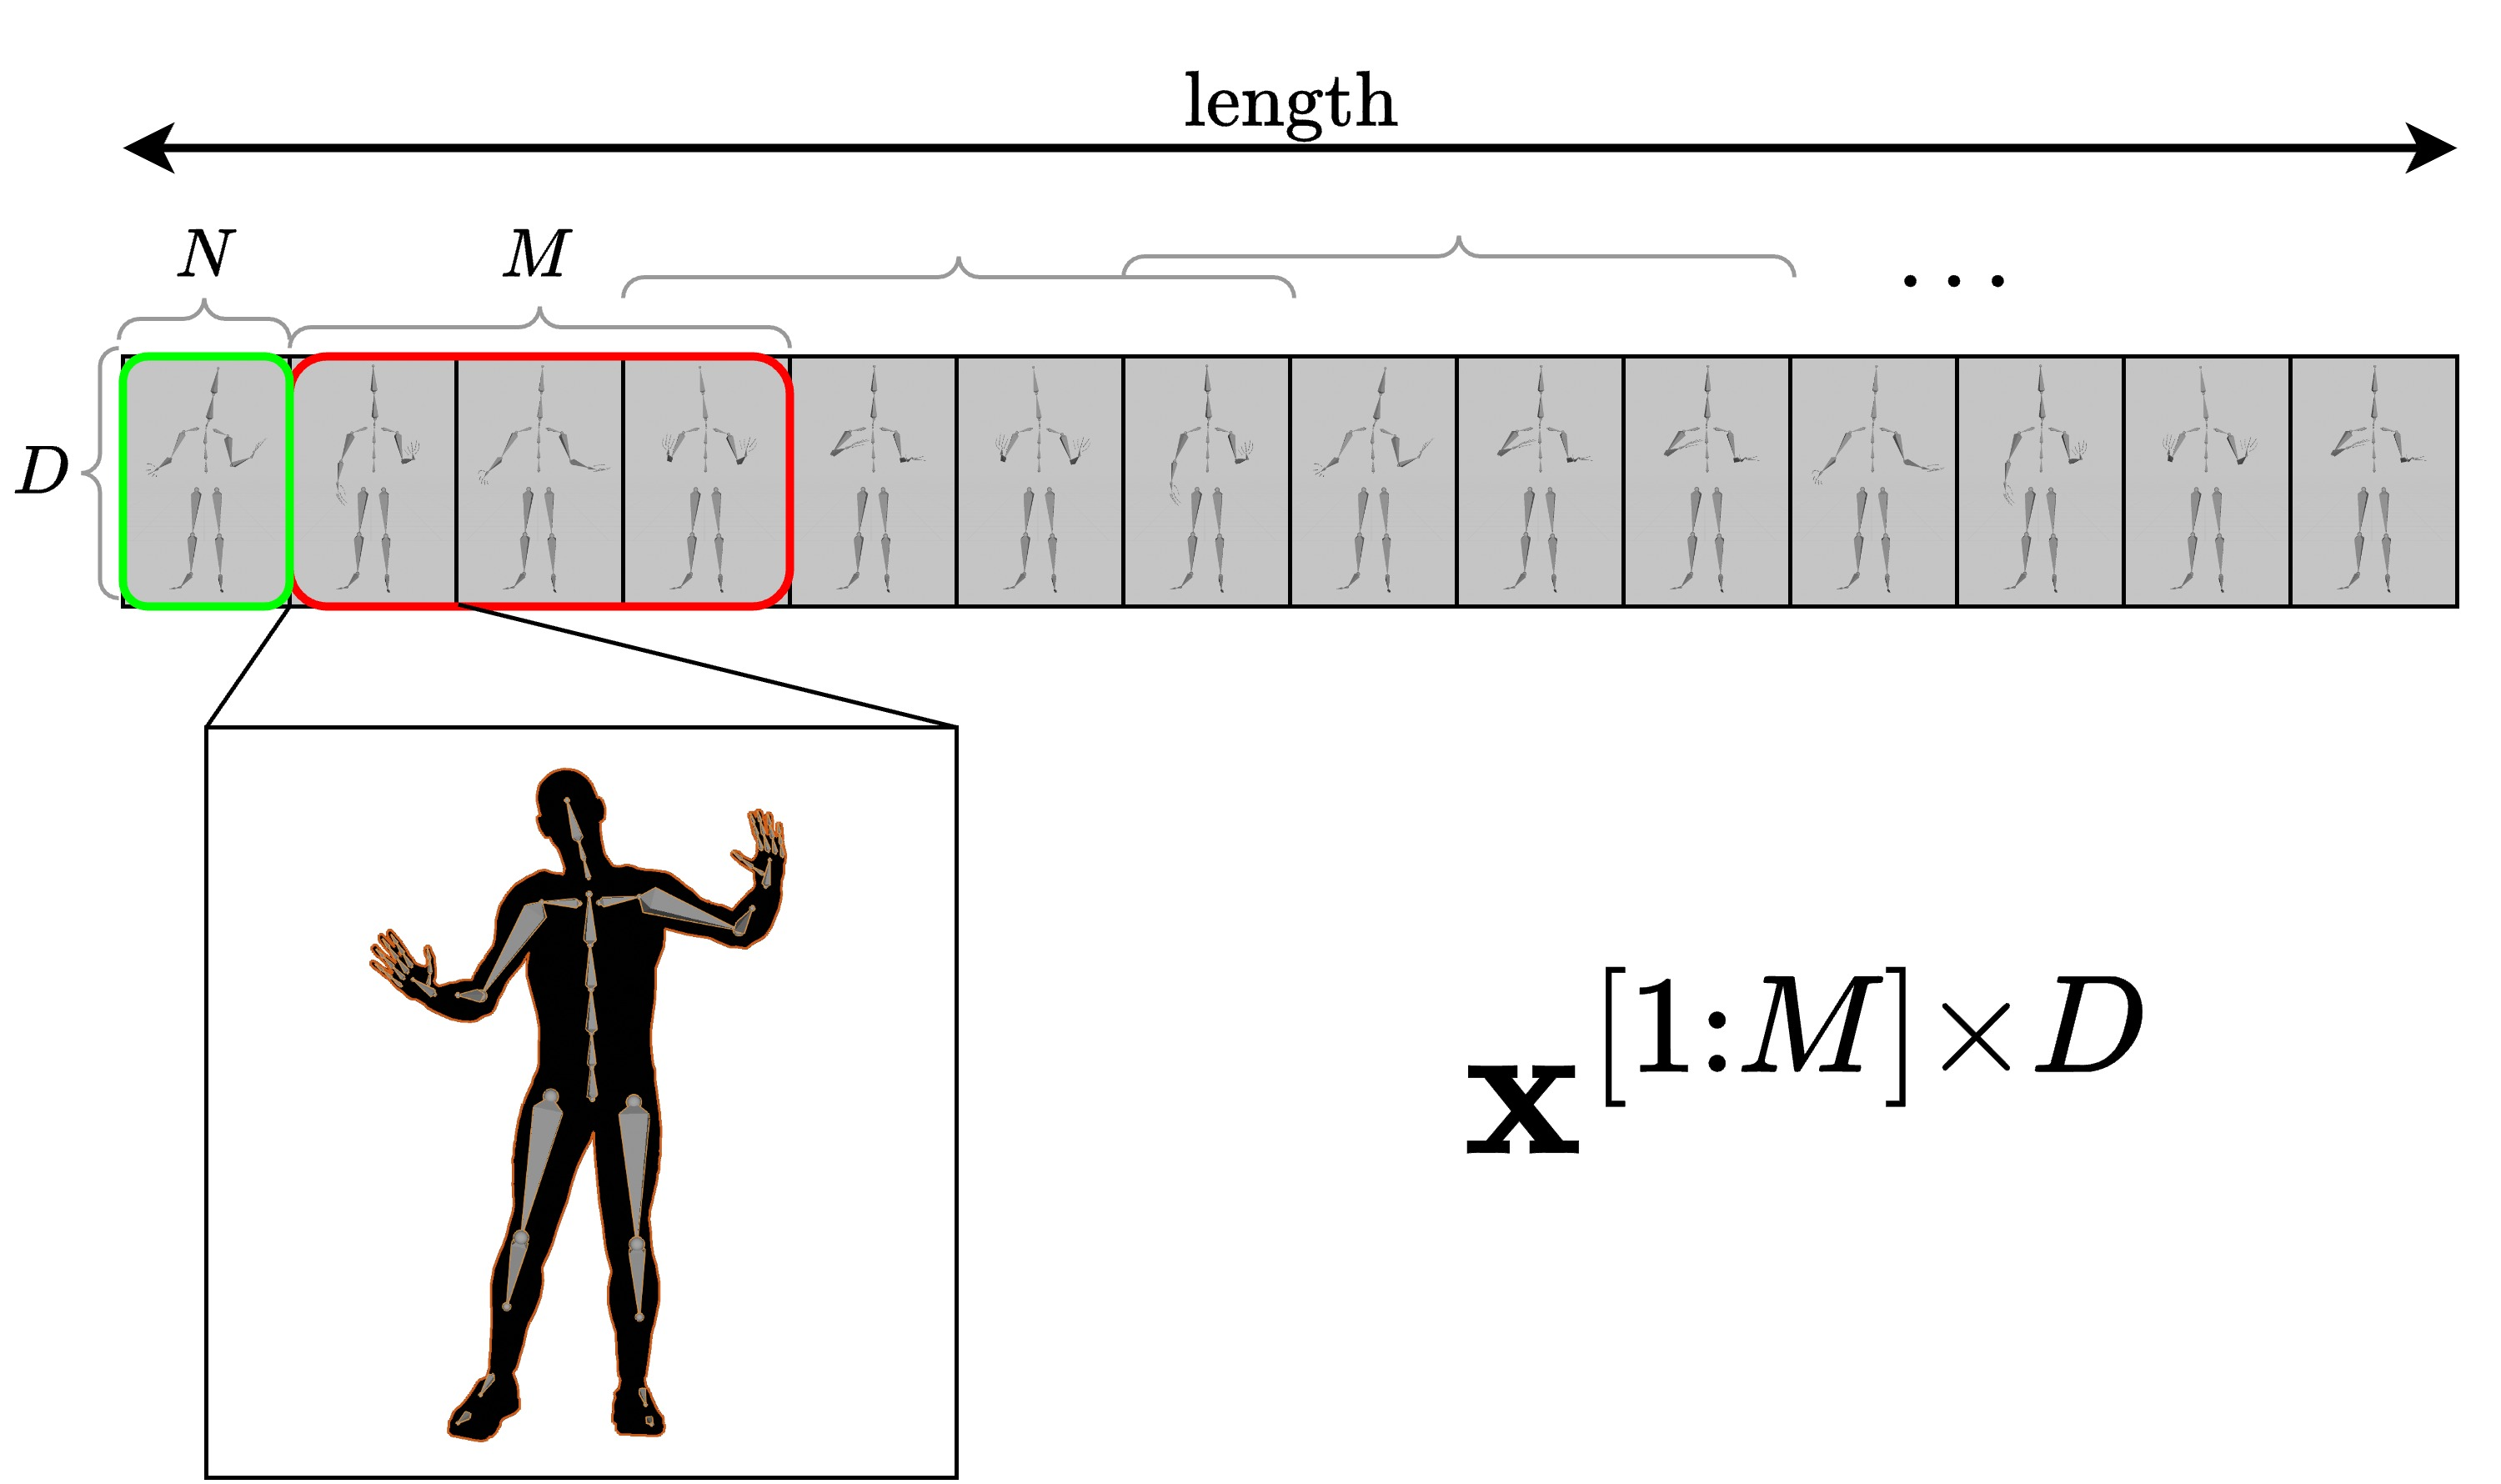
\includegraphics[width=\textwidth]{GestureFrame}
	\end{figure}
	
%{\large 
\begin{equation*}
\mathbf{g}^{[1:\operatorname{length}] \times 75 \times 6} \xrightarrow{ \text{Xử lý} }  \mathbf{g}^{[1: \operatorname{length}] \times D} \xrightarrow{ \text{Cắt} } \mathbf{g}^{[N + M] \times D}
\end{equation*}

%\textbf{Dữ liệu}
%{\Large
%	\begin{equation*}
%		\mathbf{x}^{[1:M] \times D}
%	\end{equation*}
%}

%\begin{itemize}
%	\item $[1:M]$: từ frame $1$ đến frame thứ $M$
%	\item Mỗi frame chứa đặc trưng $D$
%	%				$D = 1141$
%\end{itemize}
\end{frame}



\begin{frame}{Phát biểu bài toán}
%	\begin{figure}[h]
%		\centering
%		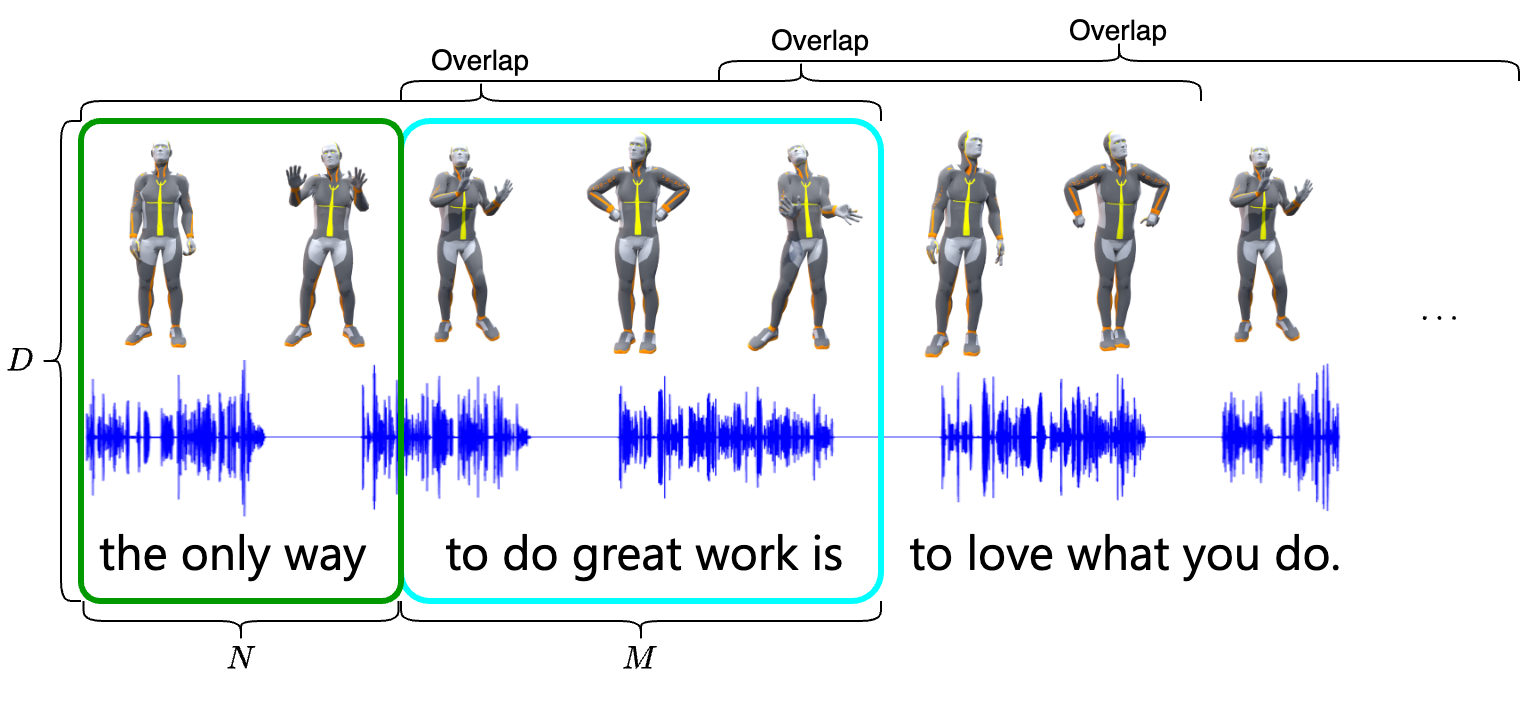
\includegraphics[height=4.5cm]{GestureSeries}
%	\end{figure}
 \vspace{-25pt}
	\begin{figure}
		\centering
		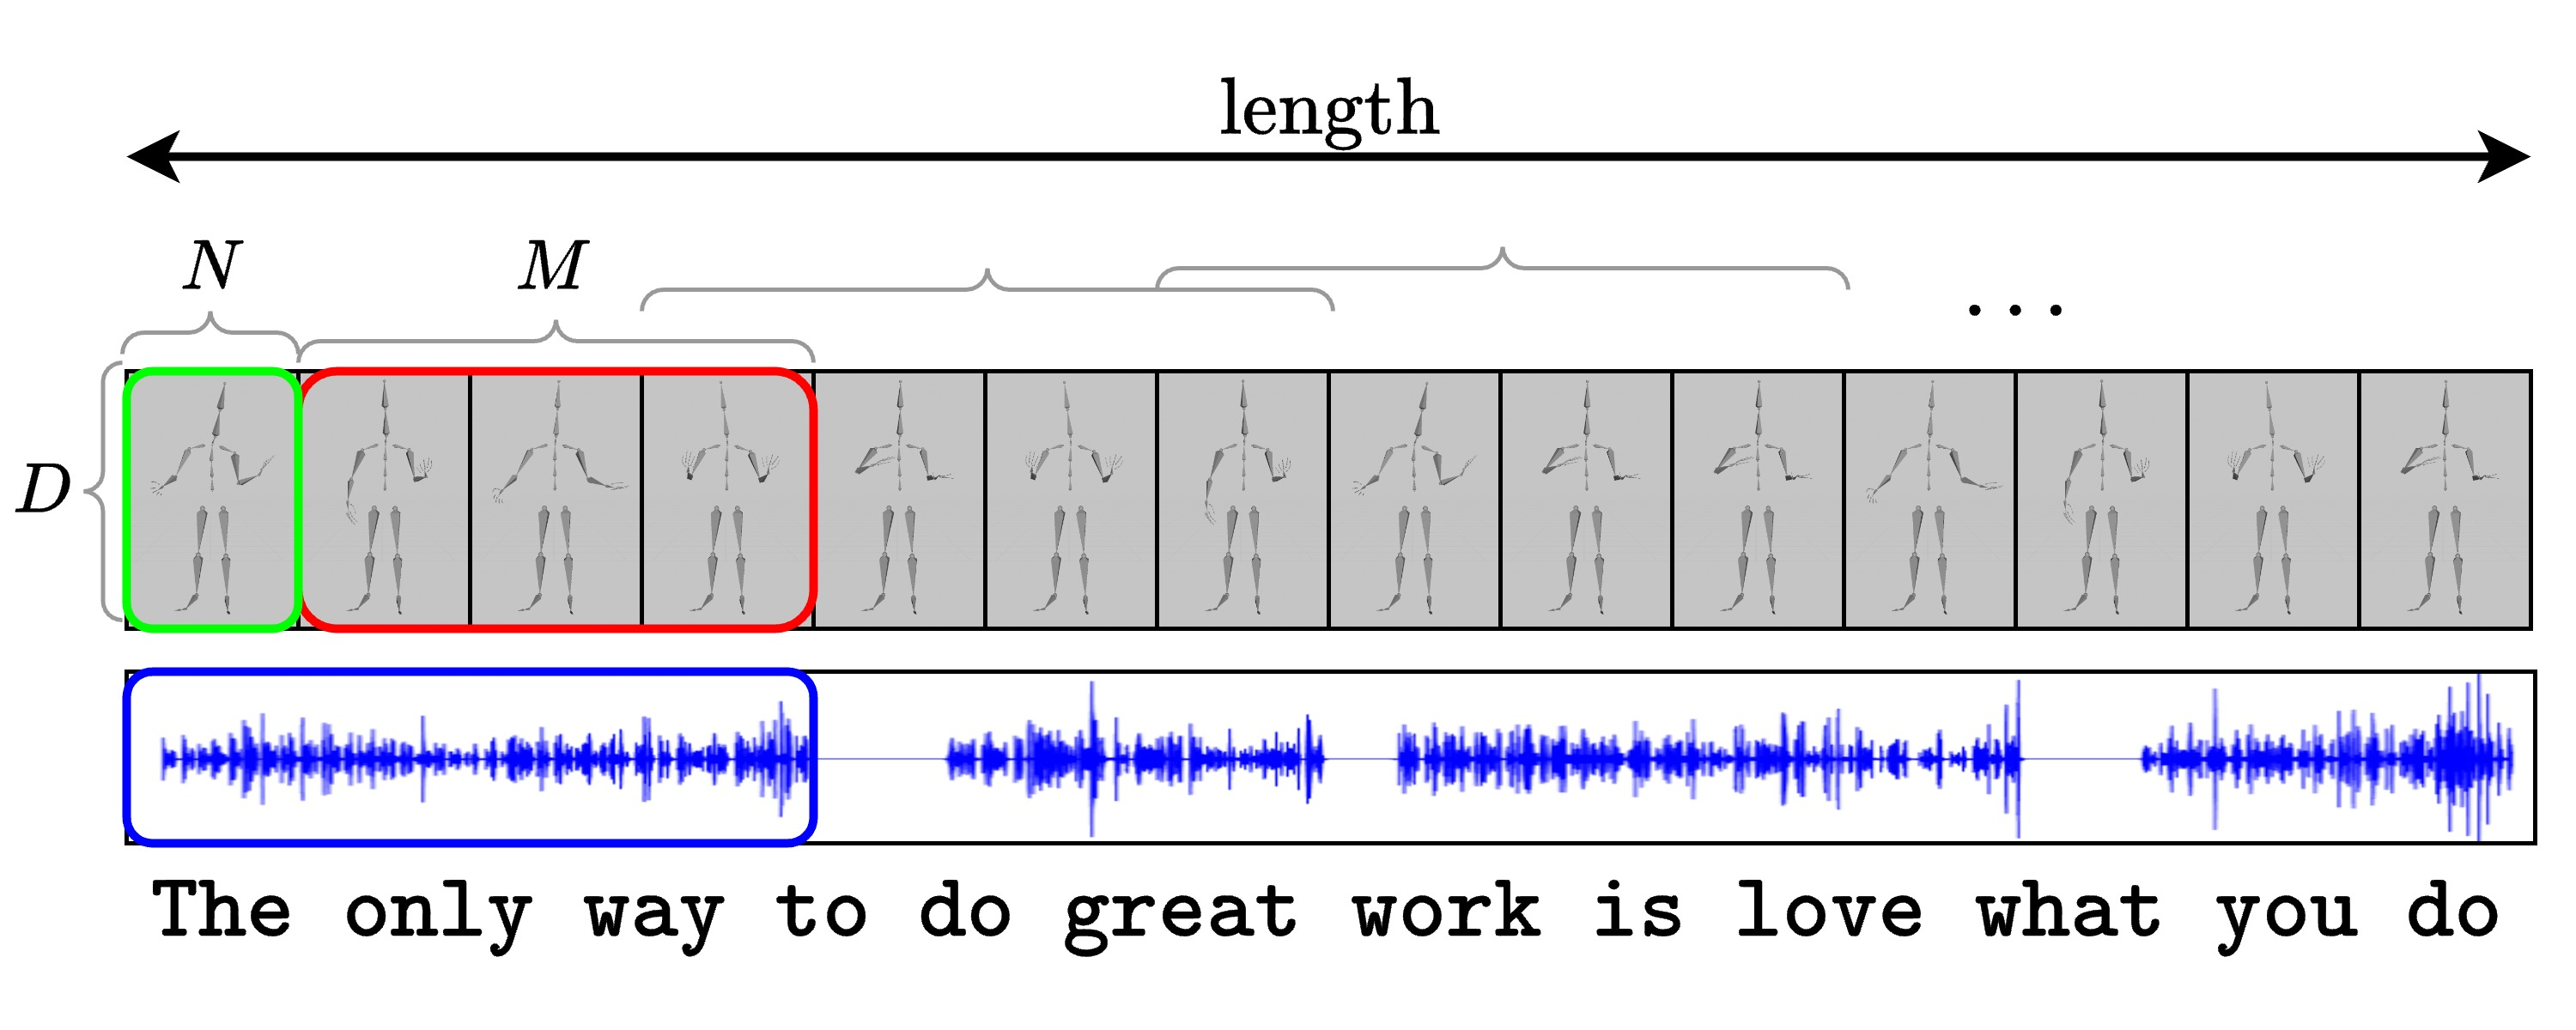
\includegraphics[width=0.95\textwidth]{FeatureProcessing}
	\end{figure}
		\vspace{20pt}
	\begin{columns}
		
	\begin{column}{0.6\textwidth}
		
		\textbf{Input}
		\begin{itemize}
			\item Chuỗi cử chỉ khởi tạo: $\mathbf{s} \in \mathbb{R}^{[1:N] \times D}$
			\item Chuỗi âm thanh: $\mathbf{a}$
			\item Văn bản: $\mathbf{v}$ 
%				\in \mathbb{R}^{16000 M}
			%			trích xuất đặc trưng MFCC: $\mathbf{a} \in \mathbb{R}^{M \times C_{\text{mfcc}}}$
			\item Cảm xúc: $\mathbf{e}$ 
			
			{\small
				(\texttt{Happy},  \texttt{Sad},  \texttt{Neutral}, \texttt{Angry}, \texttt{Old}, \texttt{Funny})
			}
%				 $\text{"Love what you do"}$
		\end{itemize}
		
	\end{column}

	\begin{column}{0.4\textwidth}
		\textbf{Output}
		\begin{itemize}
			\item Chuỗi cử chỉ dự đoán: $\hat{\mathbf{x}} \in \mathbb{R}^{[1:M] \times D}$
		\end{itemize}
		
		\textbf{Grouth Truth}
		\begin{itemize}
			\item Chuỗi cử chỉ gốc: $ \mathbf{x}  \in \mathbb{R}^{[1:M] \times D}$
		\end{itemize}
	\end{column}
\end{columns}
	
\end{frame}




\begin{frame}{Các công đoạn}
	\begin{figure}[h]
		\centering
		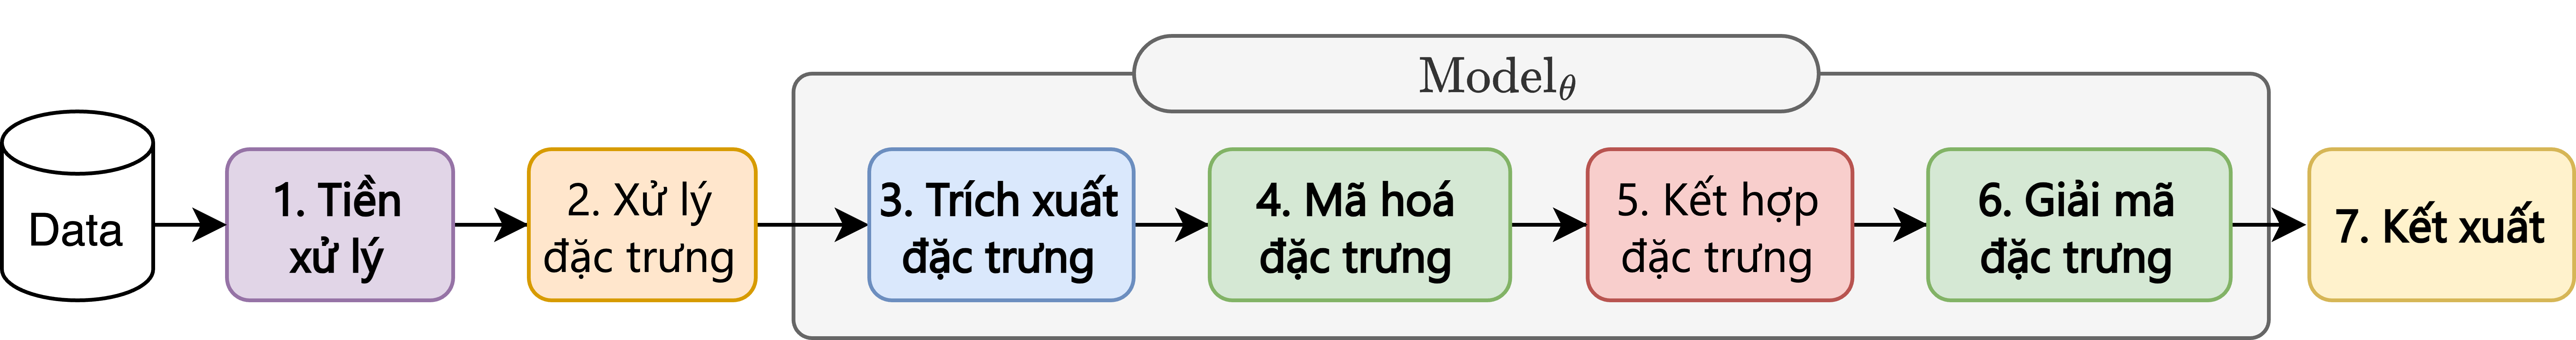
\includegraphics[width=\textwidth]{TotalStage}
	\end{figure}
\end{frame}


\begin{frame}{Công đoạn 1: Tiền xử lý dữ liệu}
%	\begin{equation*}
%		\mathbf{g} \in \mathbb{R}^{[1: \text{length} ] \times (75 \times {\{p_x, p_y, p_z, r_x, r_y, r_z\}})} \xrightarrow{\text{pre-processing}}  \mathbb{R}^{[1: \text{length}] \times D}
%	\end{equation*}
	\begin{figure}
		\centering
		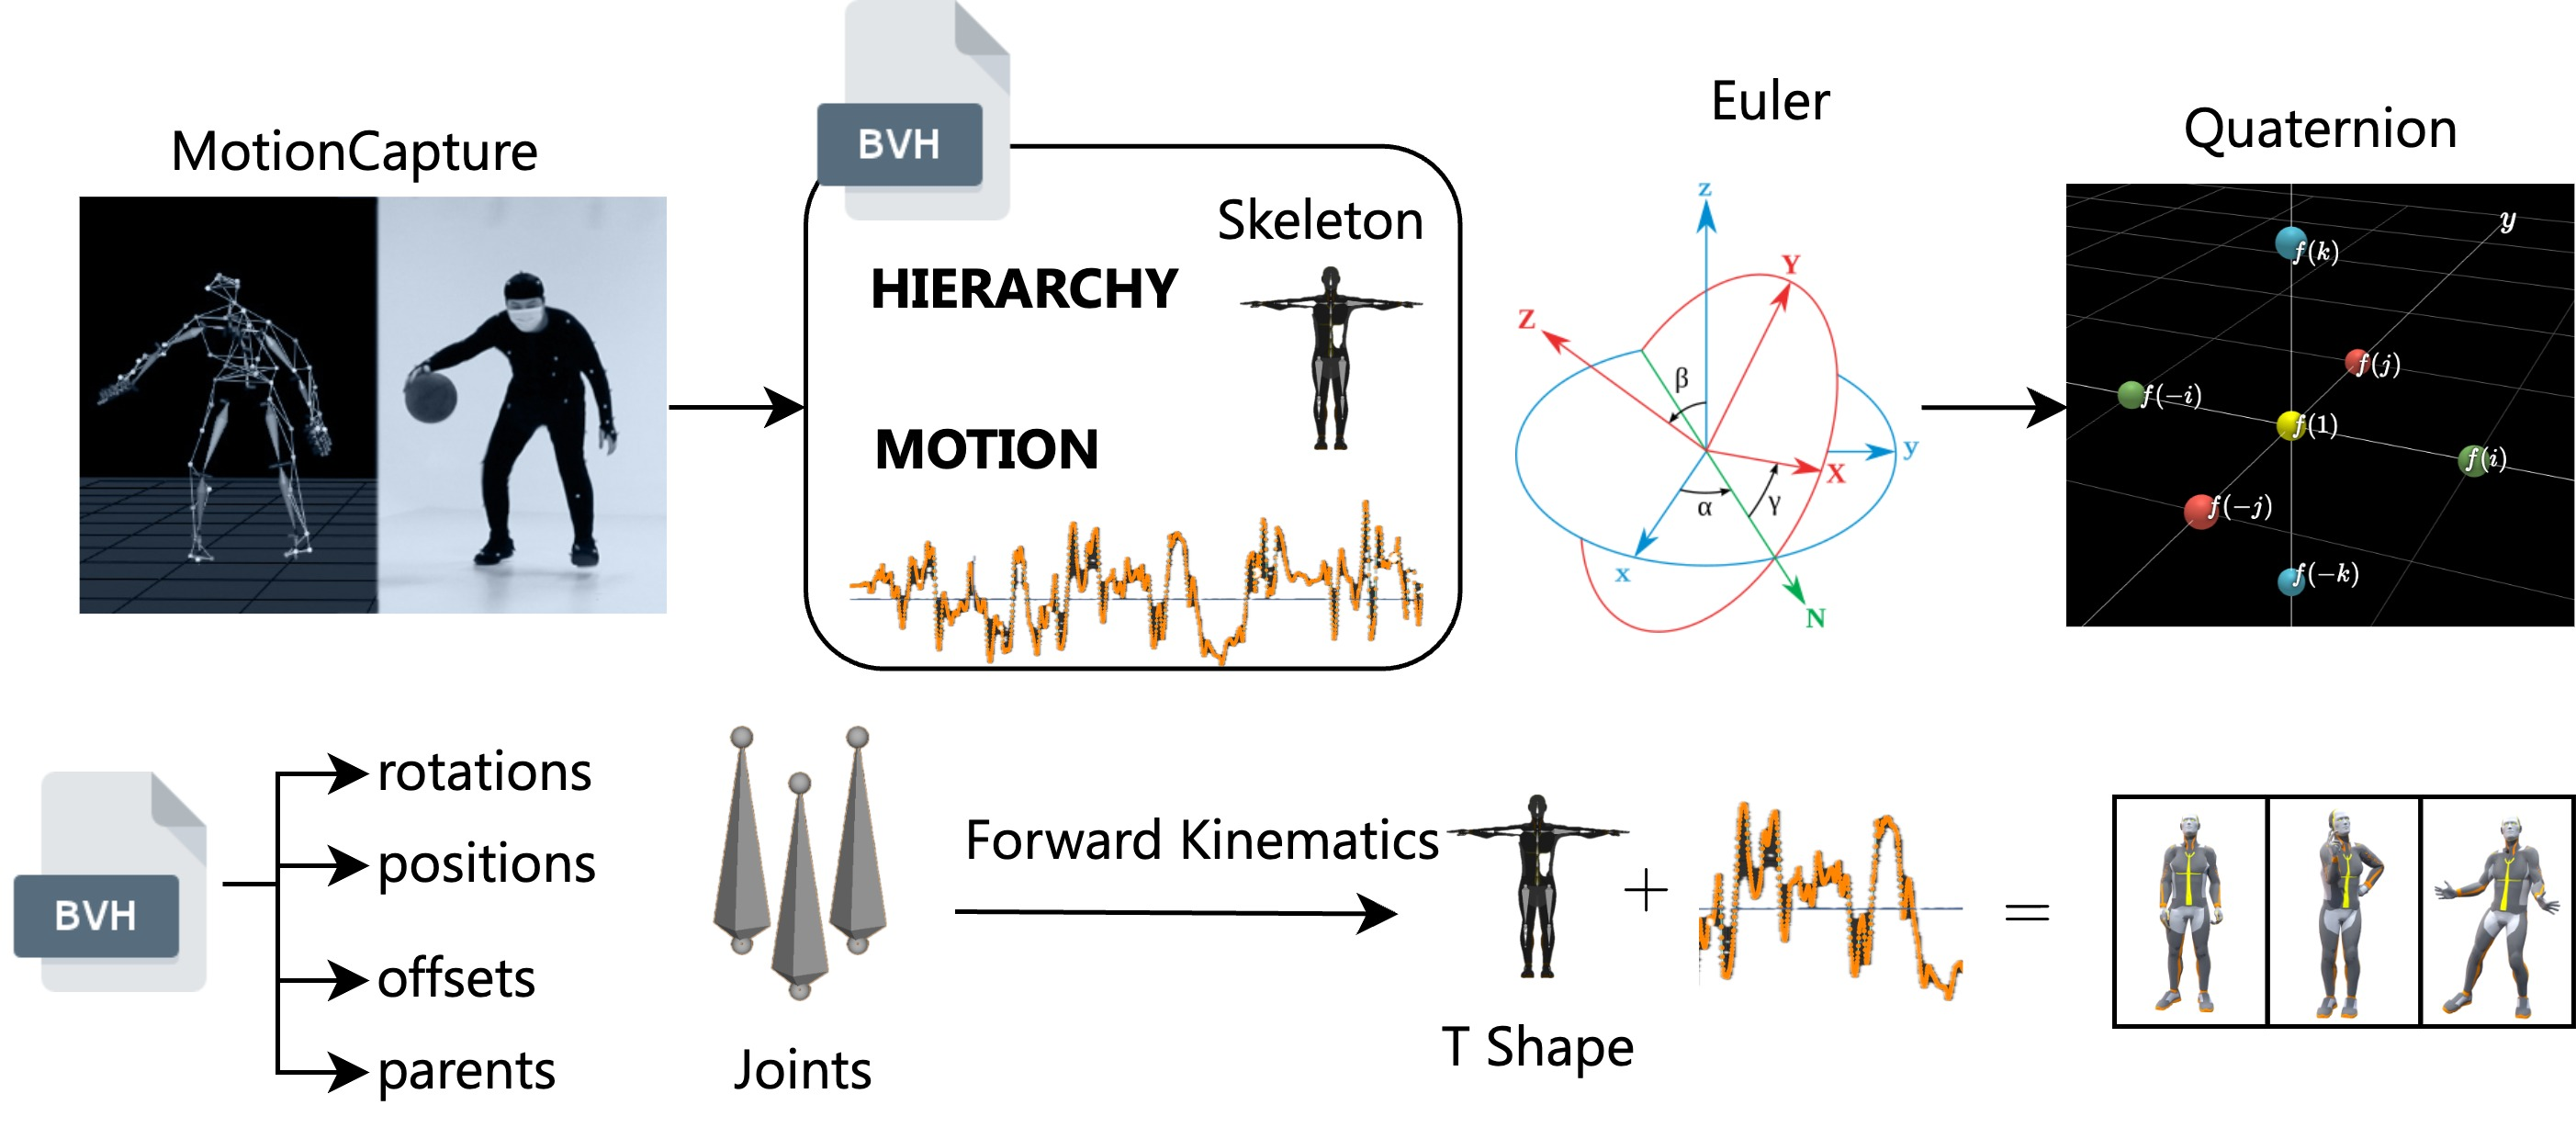
\includegraphics[width=\textwidth]{Preprocessing}
	\end{figure}
	
\end{frame}



\begin{frame}{Đặc trưng dữ liệu của $1$ frame}
	\begin{figure}
		\centering
		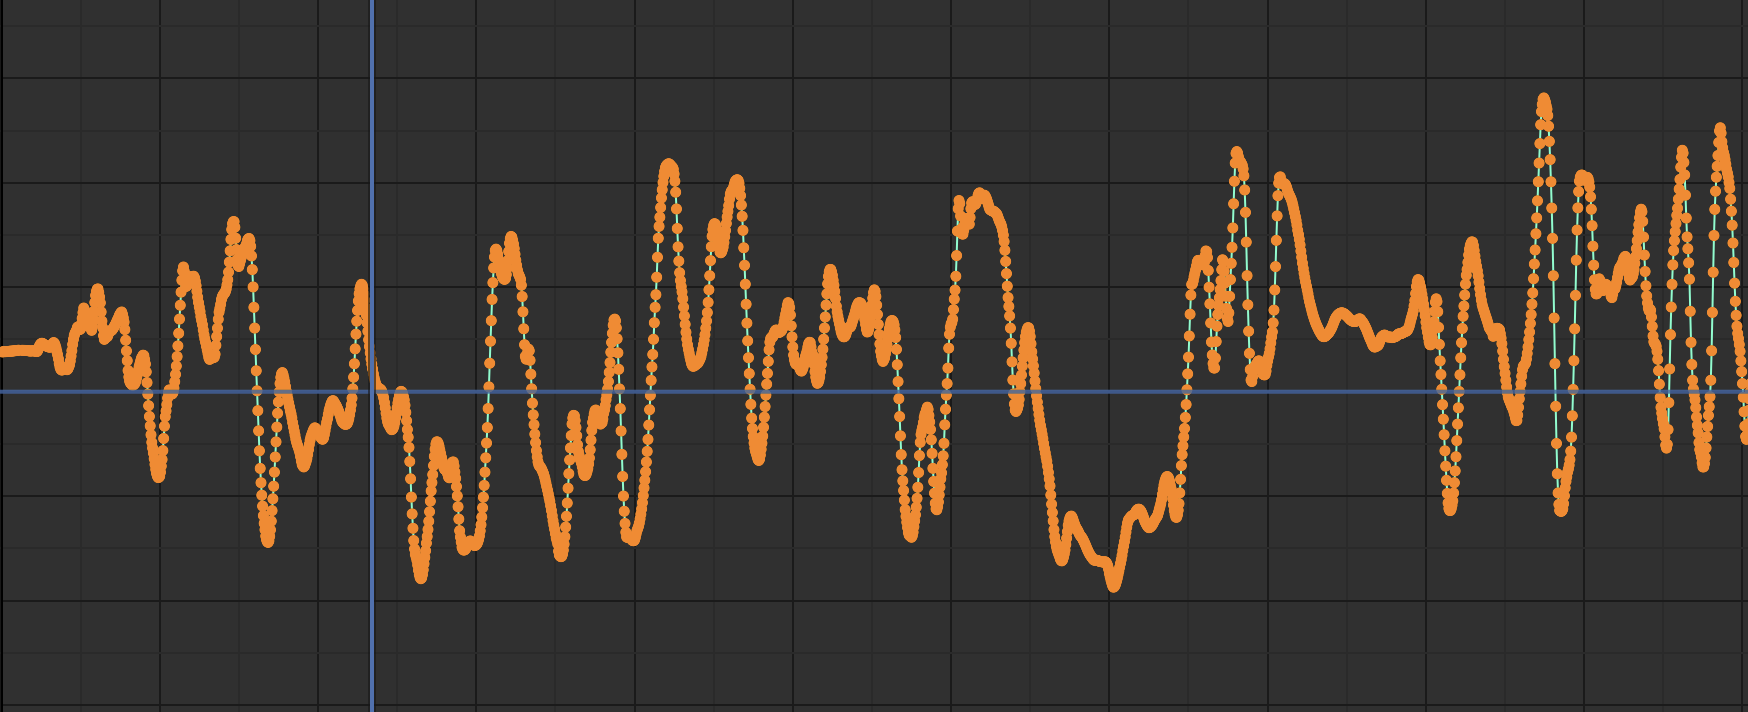
\includegraphics[width=\textwidth, height=60pt]{MotionXYZ.png}
		%		\caption{Minh hoạ chuyển động của góc quay một xương trong toạ độ}
	\end{figure}
	\begin{equation}
		\mathbf{g}^{[1]} = \Big[ \mathbf{p}_{\text{root}},  \mathbf{r}_{\text{root}},
		\mathbf{ p }'_{\text{root}},  \mathbf{r}'_{\text{root}},
		\mathbf{p}_{\text{joins}},  \mathbf{r}_{\text{joins}},
		\mathbf{p}'_{\text{joins}},  \mathbf{r}'_{\text{joins}},
		\mathbf{d}_{\text{gaze}}
		\Big]
	\end{equation}
	\vspace{-10pt}
	
	{\small
		\begin{itemize}
			\item $\mathbf{p}_{\text{root}} \in \mathbb{R}^3$, $\mathbf{r}_{\text{root}} \in \mathbb{R}^4$: Toạ độ và góc quay của điểm gốc
			\item $\mathbf{p}'_{\text{root}} \in \mathbb{R}^3$, $\mathbf{r}'_{\text{root}} \in \mathbb{R}^3$: Vận tốc thay đổi của toạ độ và góc quay gốc
			%		\item : quay
			%		Vận tốc thay đổi của góc quay gốc
			\item $\mathbf{p}_{\text{joins}} \in \mathbb{R}^{3 n_{\text{join} }}$, $\mathbf{r}_{\text{joins}} \in \mathbb{R}^{6 n_{\text{join} }}$: Toạ độ và góc quay của các khung xương
			%		\item : Góc quay của các khung xương
			\item $\mathbf{p}'_{\text{joins}} \in \mathbb{R}^{3n_{\text{join} }}$ và $\mathbf{r}'_{\text{joins}} \in \mathbb{R}^{3n_{\text{join} }}$: Vận tốc thay đổi của toạ độ và góc quay khung xương
			%		\item $\mathbf{r}'_{\text{joins}} \in \mathbb{R}^{3n_{\text{join} }}$: Vận tốc thay đổi của góc quay khung xương
			\item $\mathbf{d}_{\text{gaze}} \in \mathbb{R}^3$: Là hướng nhìn
	\end{itemize}}
	\vspace{-10pt}
	{\small
		\begin{equation*}
			D = 3 + 4 + 3 + 3 + 3 \times 75 + 6 \times 75 + 3 \times 75 + 3 \times 75 + 3 = 1141
	\end{equation*}}
	%	\begin{columns}
		%		\begin{column}{0.78\textwidth}
			
			%			$$
			%			D = 1141
			%			$$
			
			%		\end{column}
		%		
		%		\begin{column}{0.22\textwidth}
			%			\vspace{12pt}
			%			\begin{figure}
				%				\centering
				%				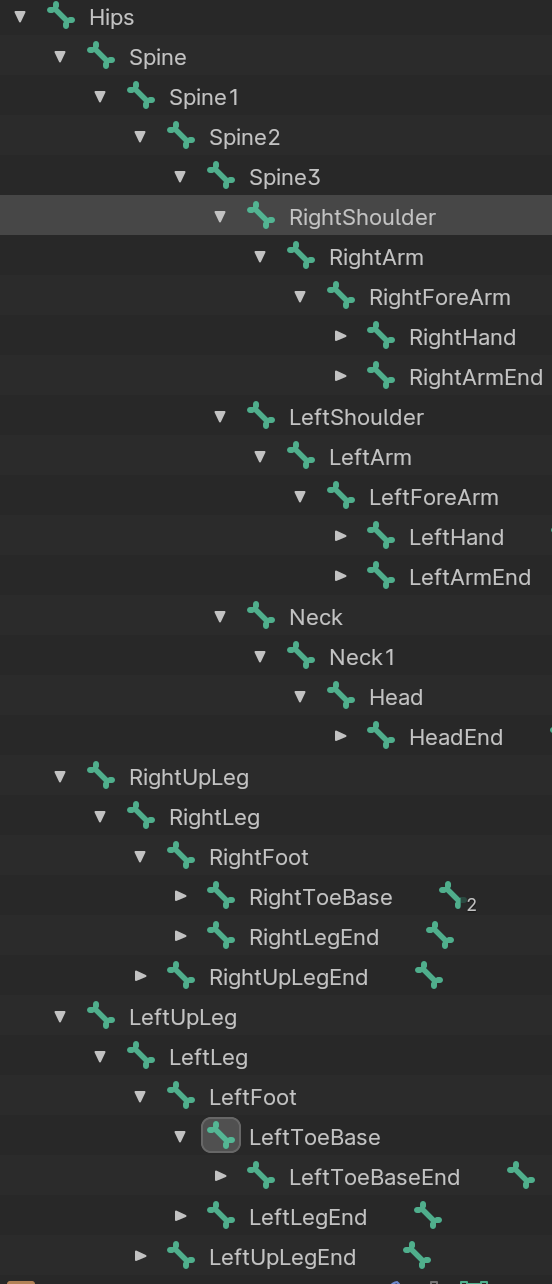
\includegraphics[width=\textwidth]{Bone.png}
				%			\end{figure}
			%			
			%		\end{column}
		%	\end{columns}
	
\end{frame}




\begin{frame}{Thách thức của bài toán}
	
	%	\begin{columns}
		%		\begin{column}{0.55\textwidth}
			%			
			%			
			%			%		\textit{Mô hình Diffusion}:
			%			%		\begin{itemize}
				%				%			\item Ít yêu cầu về dữ liệu gắn nhãn
				%				%			\item Khả năng tương tác và điều chỉnh dễ dàng
				%				%			\item Tính ổn định cao
				%				%		\end{itemize}
			%		\end{column}
		%		\begin{column}{0.45\textwidth}
			%			
			%			\begin{columns}
				%				\begin{column}{0.5\textwidth}
					%					\begin{figure}
						%						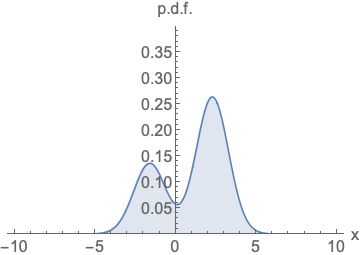
\includegraphics[width=\textwidth]{ProbabilityDensityFunctions.png}
						%						\caption{\scriptsize Phải chuẩn hoá (diện tích dưới đường cong phải tích phân thành một)}
						%					\end{figure}
					%				\end{column}
				%				\begin{column}{0.5\textwidth}
					%					\begin{figure}
						%						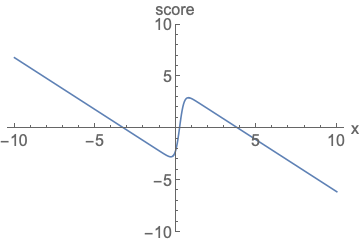
\includegraphics[width=\textwidth]{ScoreFunction.png}
						%						\caption{\scriptsize Không cần chuẩn hoá.}
						%					\end{figure}
					%				\end{column}
				%			\end{columns}
			%			
			%			
			%			
			%			\begin{columns}
				%				\begin{column}{0.5\textwidth}
					%					\centering
					%					\begin{tikzpicture}
						%						\node at (0, 1) {$p(\mathbf{x})$};
						%						
						%						\node at (0, 0.5) {\small \text{probability density}};
						%						
						%						\draw[<->, thick] (0, 0) -- (0, -0.5);
						%						
						%						\node at (0, -1) {$\nabla_\mathbf{x} \log p(\mathbf{x})$};
						%						
						%						\node at (0, -1.5) {\small \text{score function}};
						%					\end{tikzpicture}
					%					
					%				\end{column}
				%				\begin{column}{0.5\textwidth}
					%					\begin{figure}
						%						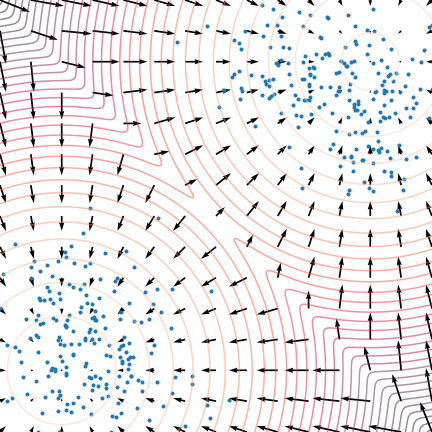
\includegraphics[width=\textwidth]{CompareScoreFunction.png}
						%						\caption{\scriptsize score function vs probability density}
						%					\end{figure}
					%				\end{column}
				%			\end{columns}
			%		\end{column}
		%	\end{columns}
	\textbf{Quan hệ giữa dữ liệu cử chỉ và âm thanh}:
	\begin{itemize}
		\item Quan hệ n:n của âm thanh, cử chỉ, cảm xúc.
	\end{itemize}
	%		Baseline: \textbf{MDM}  (Human Motion Diffusion Model)
	\textbf{Khó khăn}
	\begin{enumerate}
		\item Dữ liệu không đủ nhiều và chất lượng, chi phí cao
		\item Không cân xứng về dữ liệu giữa các loại đăng trưng cần học (âm thanh, cử chỉ)
		\item Thiếu đồng nhất của về ngữ cảnh của các loại dữ liệu
		%				\item Quá trình sinh có thể dể điều khiển 
		%			hơn GAN.
	\end{enumerate}
	%	$\rightarrow$  \textbf{DiffuseStyleGesture}: Diffusion cho bài toán sinh cử chỉ
\end{frame}


%
%\begin{frame}{Đóng góp}
%
%\end{frame}
%\[
%\begin{array}{ll}
%\mbox{minimize} & f(x) + \lambda \sum_{i=1}^N \|x_i\|_2
%\end{array}
%\]


%\begin{frame}{Structured group lasso \\[-0.3em] 
%{\footnotesize \textmd{(Jacob, Obozinski, Vert; Bach et al.; Zhao, Rocha, Yu; \dots)}}}
%\begin{itemize}\itemsep=12pt
%\item problem:
%\[
%\begin{array}{ll}
%\mbox{minimize} & f(x) + \sum_{i=1}^N \lambda_i \|x_{g_i}\|_2
%\end{array}
%\]
%where $g_i \subseteq [n]$ and $\mathcal G = \{g_1, \dots, g_N\}$
%\item like group lasso, but the groups can overlap arbitrarily
%\item particular choices of groups can impose `structured' sparsity
%\item \eg, topic models, selecting interaction terms for (graphical) models,
%    tree structure of gene networks, fMRI data
%\item generalizes to the \textbf{composite absolute penalties family}:
%\[
%r(x) = \|(\|x_{g_1}\|_{p_1}, \dots, \|x_{g_N}\|_{p_N})\|_{p_0}
%\]
%\end{itemize}
%\end{frame}

%\begin{frame}{Structured group lasso \\[-0.3em] 
%{\footnotesize \textmd{(Jacob, Obozinski, Vert; Bach et al.; Zhao, Rocha, Yu; \dots)}}}
%\textbf{hierarchical selection}:
%\begin{center}
%\begin{tikzpicture}
%[dot/.style={rectangle,draw=black,fill=white,inner sep=5pt,minimum size=5pt}]
%\node[dot,draw=orange,thick] at (0,5) (n1) {1};
%\node[dot] at (-1,4) (n2) {2};
%\node[dot,draw=orange,thick] at (1,4) (n3) {3};
%\node[dot] at (-1,3) (n4) {4};
%\node[dot,draw=orange,thick] at (0.5,3) (n5) {5};
%\node[dot] at (1.5,3) (n6) {6};
%\draw[->] (n1) -- (n2);
%\draw[->] (n1) -- (n3);
%\draw[->] (n2) -- (n4);
%\draw[->] (n3) -- (n5);
%\draw[->] (n3) -- (n6);
%\end{tikzpicture}
%\end{center}
%\begin{itemize}\itemsep=8pt
%    \item $\mathcal G = \{ \{4\}, \textcolor{orange}{\{5\}}, \{6\}, \{2,4\}, 
%        \textcolor{orange}{\{3,5,6\}}, \textcolor{orange}{\{1,2,3,4,5,6\} \}}$
%\item nonzero variables form a rooted and connected subtree
%    \begin{itemize}
%        \item if node is selected, so are its ancestors
%        \item if node is not selected, neither are its descendants
%    \end{itemize}
%\end{itemize}
%\end{frame}

%\begin{frame}[fragile]{Sample ADMM implementation: lasso}
%\begin{verbatim}
%prox_f = @(v,rho) (rho/(1 + rho))*(v - b) + b;
%prox_g = @(v,rho) (max(0, v - 1/rho) - max(0, -v - 1/rho));
%
%AA = A*A';
%L  = chol(eye(m) + AA);
%
%for iter = 1:MAX_ITER
%    xx = prox_g(xz - xt, rho);
%    yx = prox_f(yz - yt, rho);
%
%    yz = L \ (L' \ (A*(xx + xt) + AA*(yx + yt)));
%    xz = xx + xt + A'*(yx + yt - yz);
%  
%    xt = xt + xx - xz;
%    yt = yt + yx - yz;
%end
%\end{verbatim}
%\end{frame}

\section{Công trình liên quan}

\begin{frame}{Các phương pháp}
\textbf{Rule Base \& Statistic}
\begin{itemize}
	\small
	\item BEAT, Rule-based generation.
	%					 \cite{cassell2001beat}
	\item Gesture Controllers 
\end{itemize}
%	\textit{Nhược điểm}: Không có khả năng mở rộng, kết quả không tốt với các dữ liệu ngoài tập huấn luyện.

\textbf{Deep Learning}
%\begin{itemize}
%	\small
%	\item \textbf{MLP}: Gesticulator
%	\item \textbf{RNN}: Speech2AffectiveGestures, HA2G, TransGesture, .. 
%	\item \textbf{Normalising Flows}: Text2gestures, Speech2Gesture,; \textbf{GAN}: DiffGAN
%	\item \textbf{VAE/VQ-VAE}:  Audio2Gestures; 
%	\item \textbf{Diffusion}: Listen denoise action, DiffuseStyleGesture, Taming Diffusion Models.
%\end{itemize}
\begin{columns}
	\begin{column}{0.5\textwidth}
			{
			\small
			\textbf{Likelihood-based models}:
			\begin{itemize}
				\item \textbf{MLP}: Gesticulator
				\item \textbf{RNN}: Speech2AffectiveGestures, HA2G, TransGesture, .. 
				\item \textbf{Normalising Flows}: Text2gestures, Speech2Gesture
				\textbf{VAE/VQ-VAE}:  Audio2Gestures; 
				\end{itemize}
			}
			 \begin{figure}
				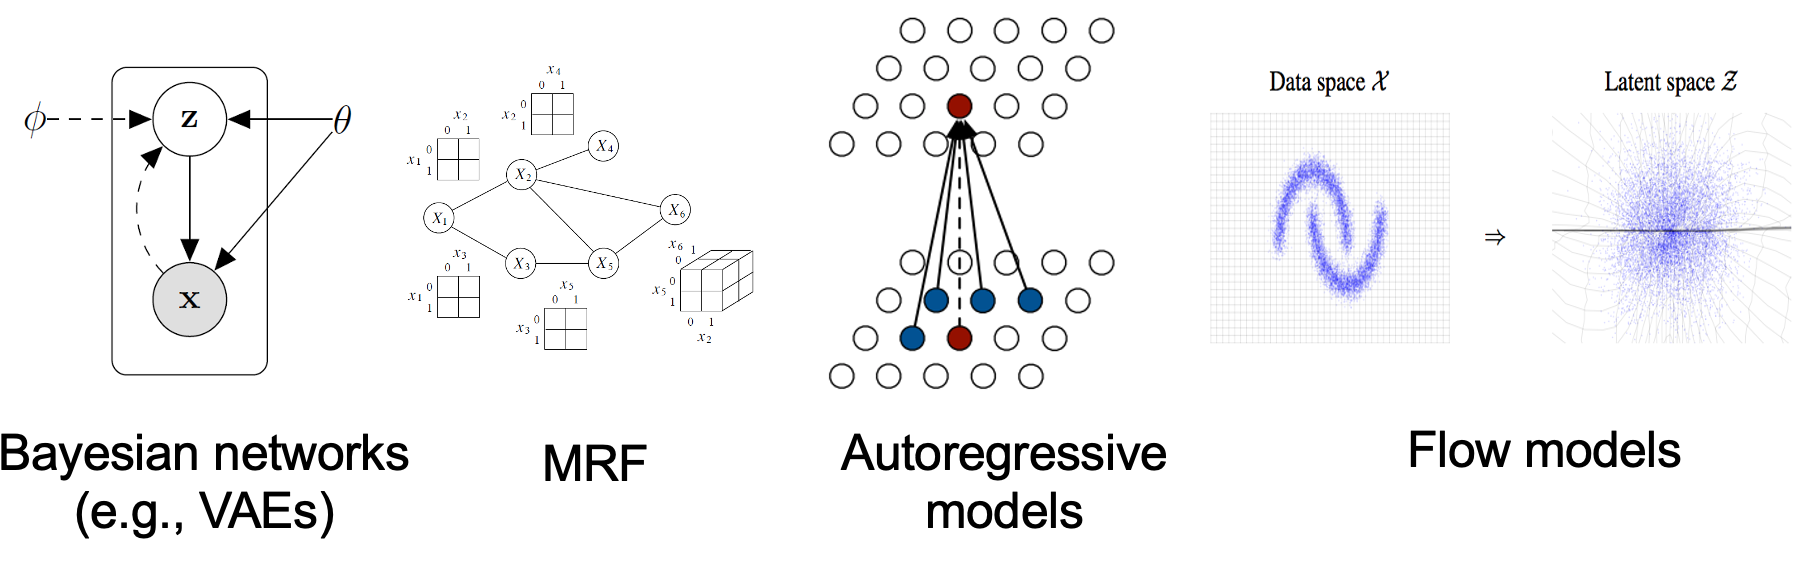
\includegraphics[width=\textwidth]{likelihood_based_models}
			\end{figure}
	\end{column}
	\hspace{-20pt}
	\begin{column}{0.5\textwidth}
		{
			\small
			\textbf{Implicit generative models}:
\begin{itemize}
			\item \textbf{GAN}: DiffGAN
			
			\item \textbf{Diffusion}: Listen denoise action, DiffuseStyleGesture, Taming Diffusion Models.
 \end{itemize}
 
 \begin{figure}
 	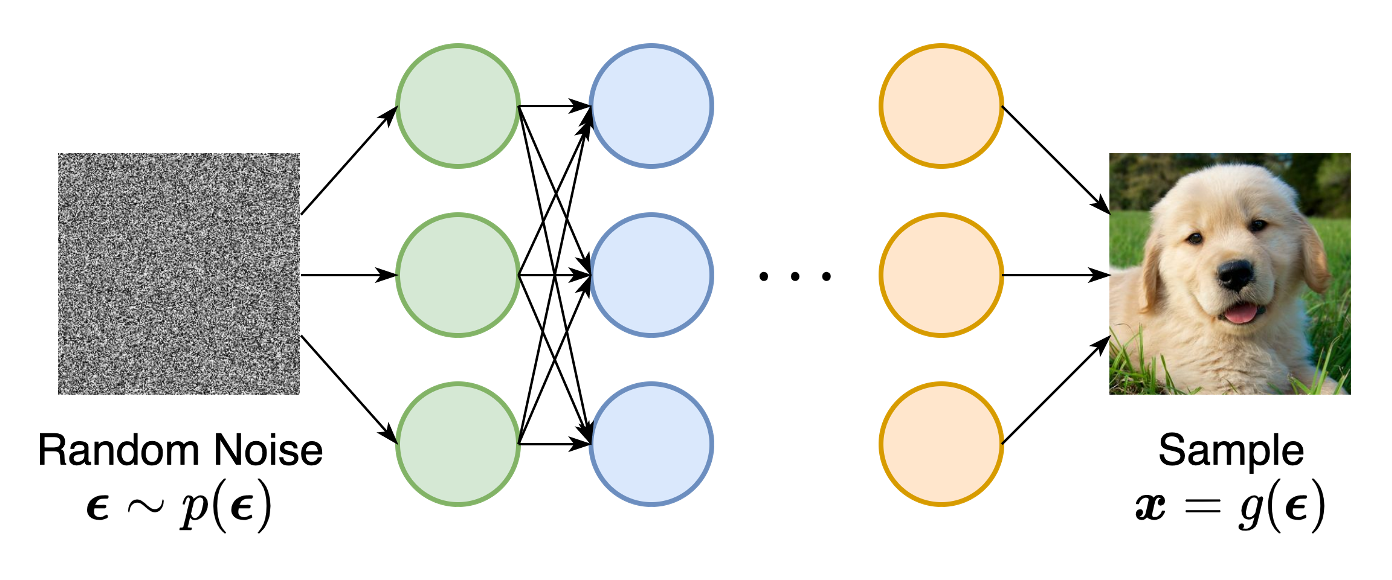
\includegraphics[width=\textwidth]{implicit_models}
 \end{figure}
 
		}
	\end{column}
\end{columns}

%	\textbf{Phase Manifold} : 
%	
%	\begin{itemize}
%		\small
%		\item  DeepPhase , Walk the Dog
%	\end{itemize}

	

%\textbf{Baseline}: \textit{Motion Diffusion Model} (MDM)

%\begin{columns}
%\begin{column}{0.55\textwidth}
	
%\end{column}			
% 
%	
%	\begin{column}{0.45\textwidth}
%		
%		\begin{columns}
%			\begin{column}{0.5\textwidth}
%				\begin{figure}
%					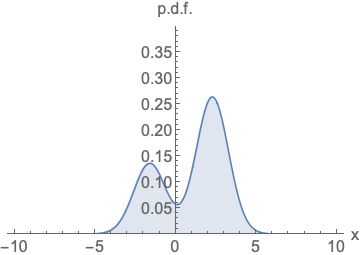
\includegraphics[width=\textwidth]{ProbabilityDensityFunctions.png}
%					\caption{\scriptsize Phải chuẩn hoá (diện tích dưới đường cong phải tích phân thành một)}
%				\end{figure}
%			\end{column}
%			\begin{column}{0.5\textwidth}
%				\begin{figure}
%					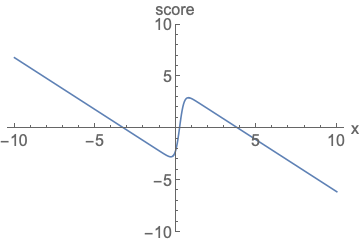
\includegraphics[width=\textwidth]{ScoreFunction.png}
%					\caption{\scriptsize Không cần chuẩn hoá.}
%				\end{figure}
%			\end{column}
%		\end{columns}
%	
%		\begin{columns}
%			\begin{column}{0.5\textwidth}
%				\centering
%				\begin{tikzpicture}
%					\node at (0, 1) {$p(\mathbf{x})$};
%					
%					\node at (0, 0.5) {\small \text{probability density}};
%					
%					\draw[<->, thick] (0, 0) -- (0, -0.5);
%					
%					\node at (0, -1) {$\nabla_\mathbf{x} \log p(\mathbf{x})$};
%					
%					\node at (0, -1.5) {\small \text{score function}};
%				\end{tikzpicture}
%				
%			\end{column}
%			\begin{column}{0.5\textwidth}
%				\begin{figure}
%					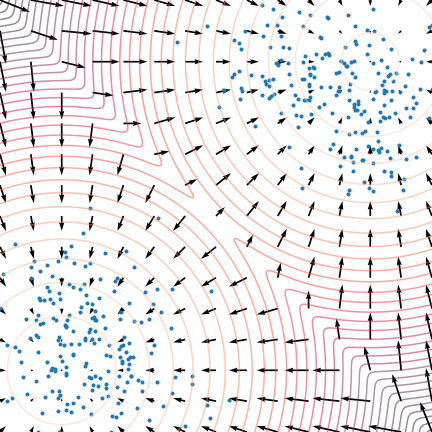
\includegraphics[width=\textwidth]{CompareScoreFunction.png}
%					\caption{\scriptsize score function vs probability density}
%				\end{figure}
%			\end{column}
%		\end{columns}
%	\end{column}
%\end{columns}

%\includegraphics[width=\linewidth]{../animation/ScoreFunction/ScoreFunction\_001}
	
\end{frame}



\begin{frame}{Tư tưởng cơ bản của Diffusion}
	Dataset $\mathcal{G} = \{ x_{i}^{M \times D} \}_{1}^{n}$, ta chuẩn hoá dữ liệu $\bx_{i}^{M \times D} = \frac{\bx_{i}^{M \times D} - \mu}{\sigma}$
\begin{figure}
	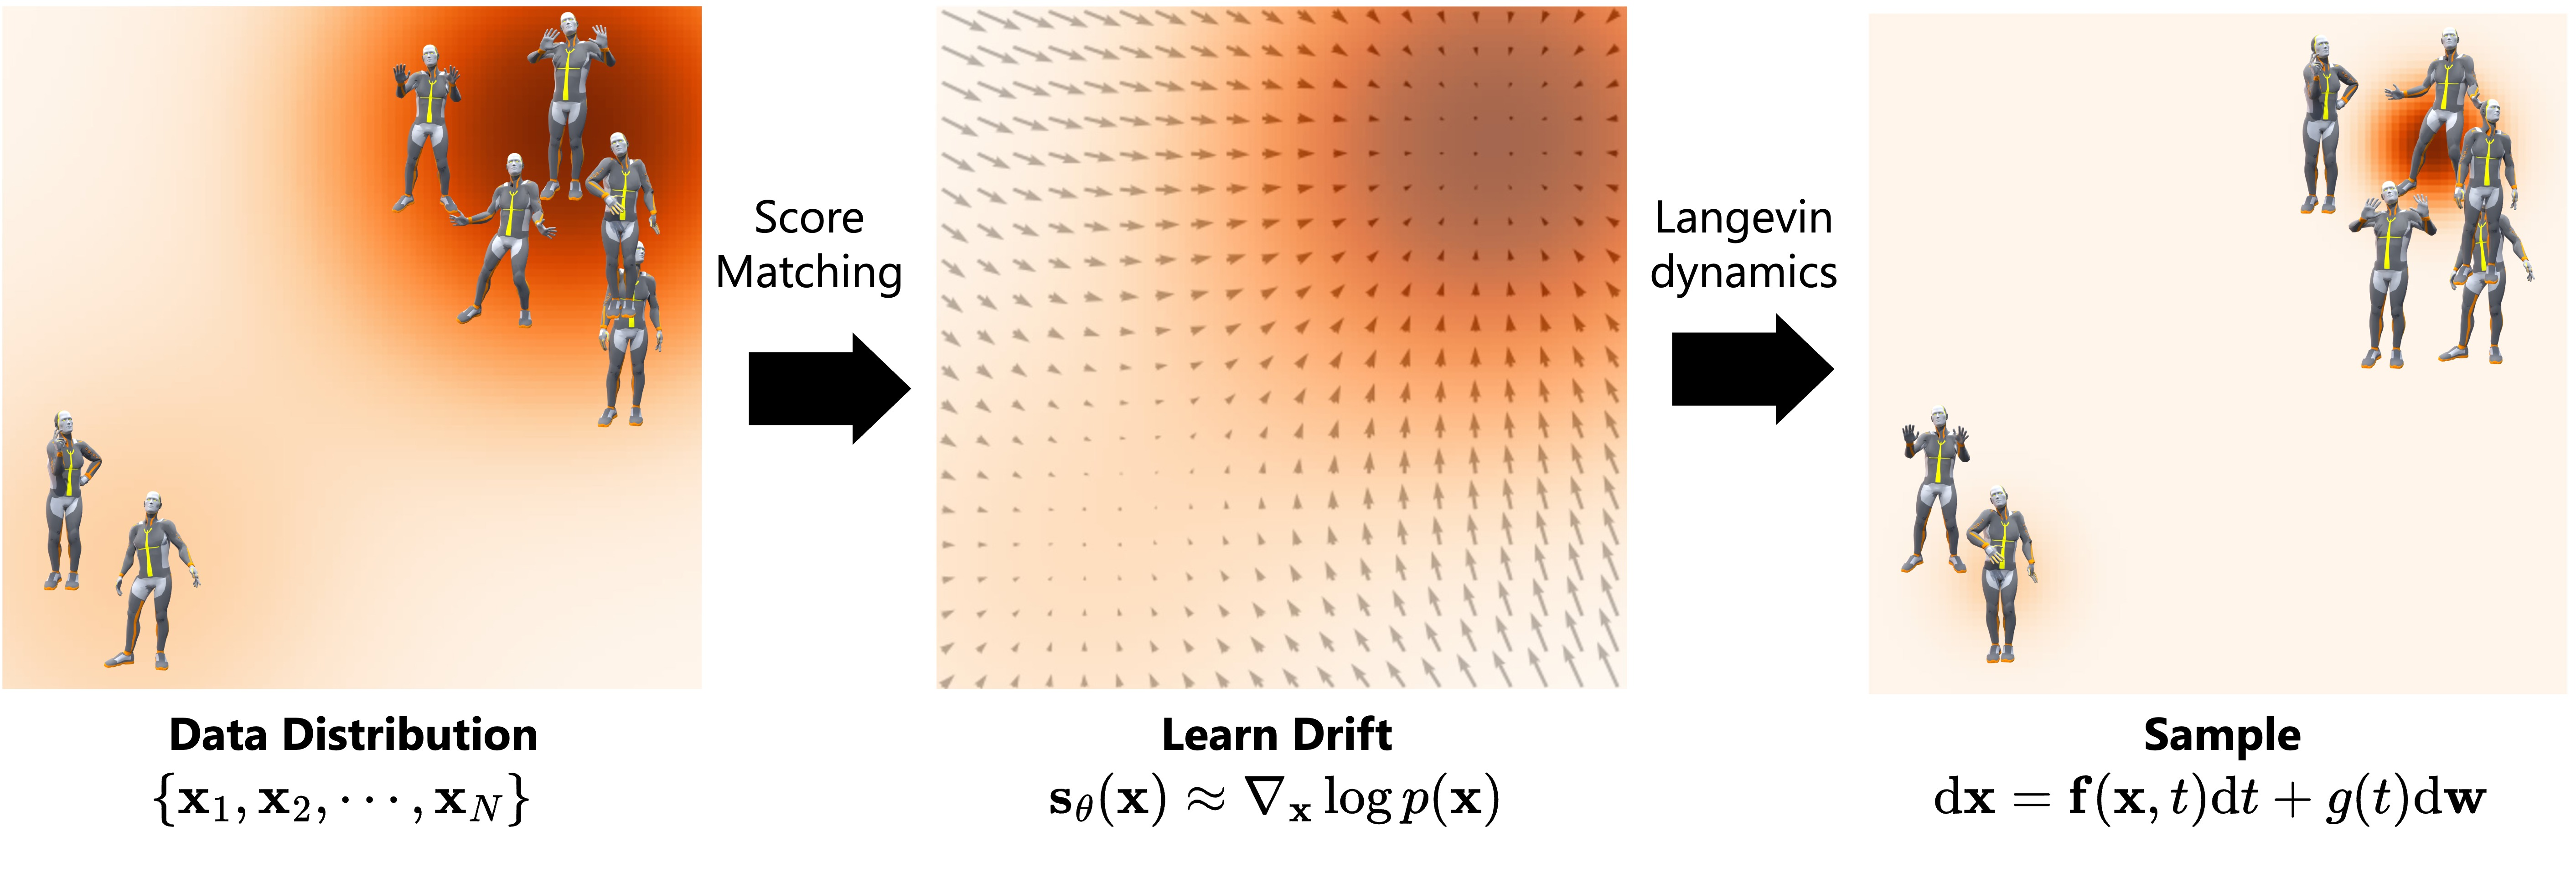
\includegraphics[width=0.8\textwidth]{ScoreMatching}
\end{figure}
\vspace{-10pt}
\begin{figure}
	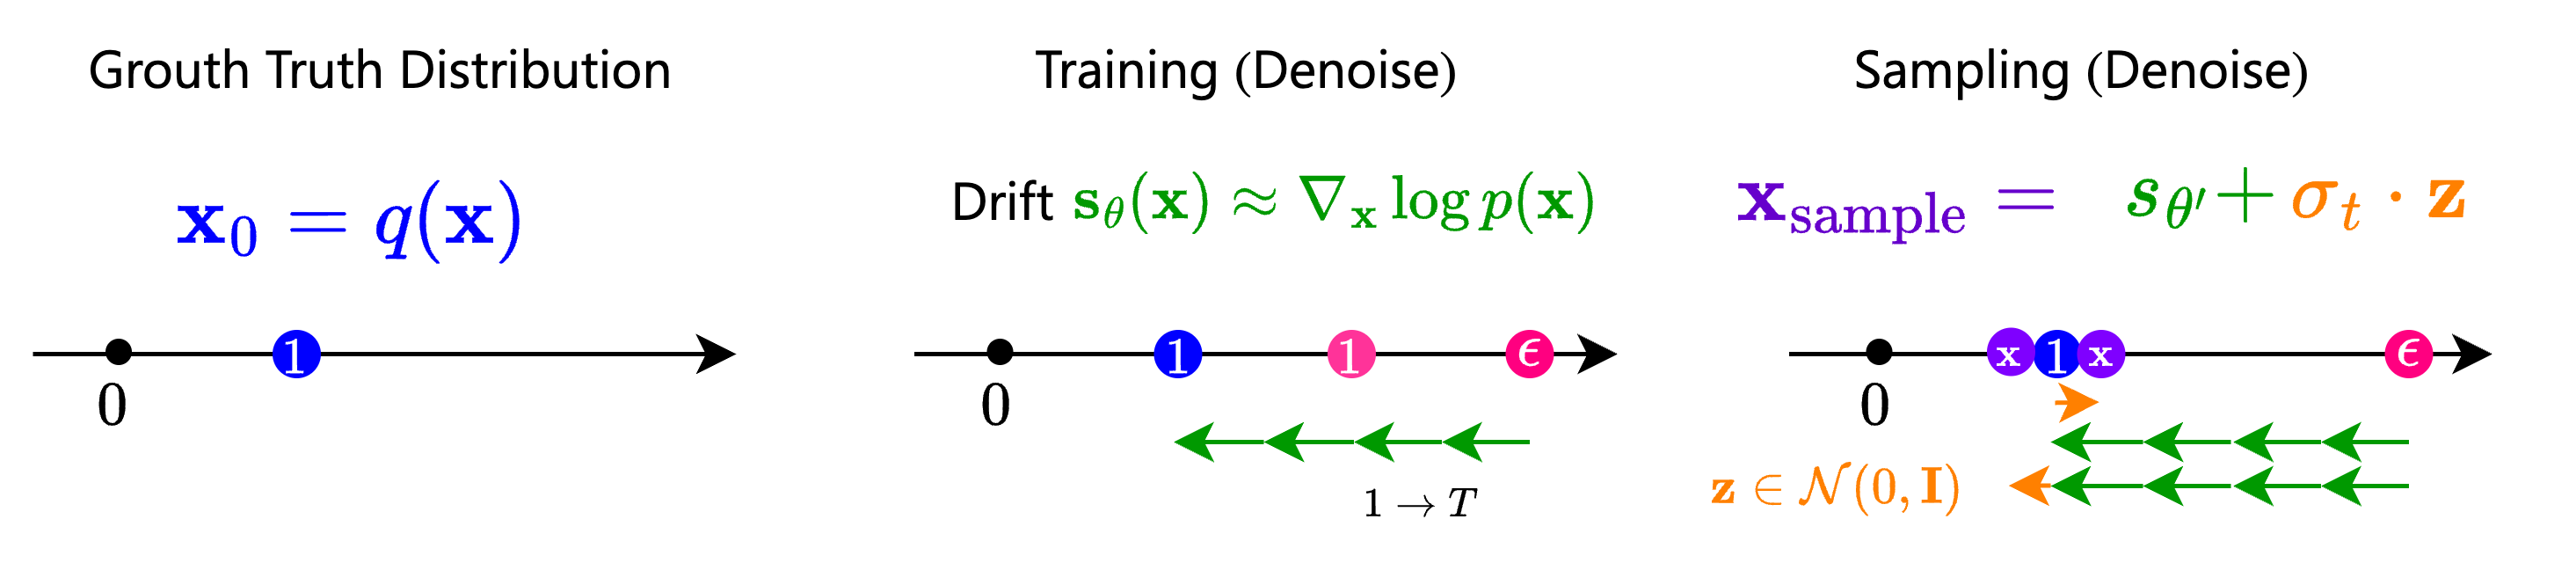
\includegraphics[width=\textwidth]{ScoreDrift}
\end{figure}

\vspace{-10pt}

\begin{figure}
	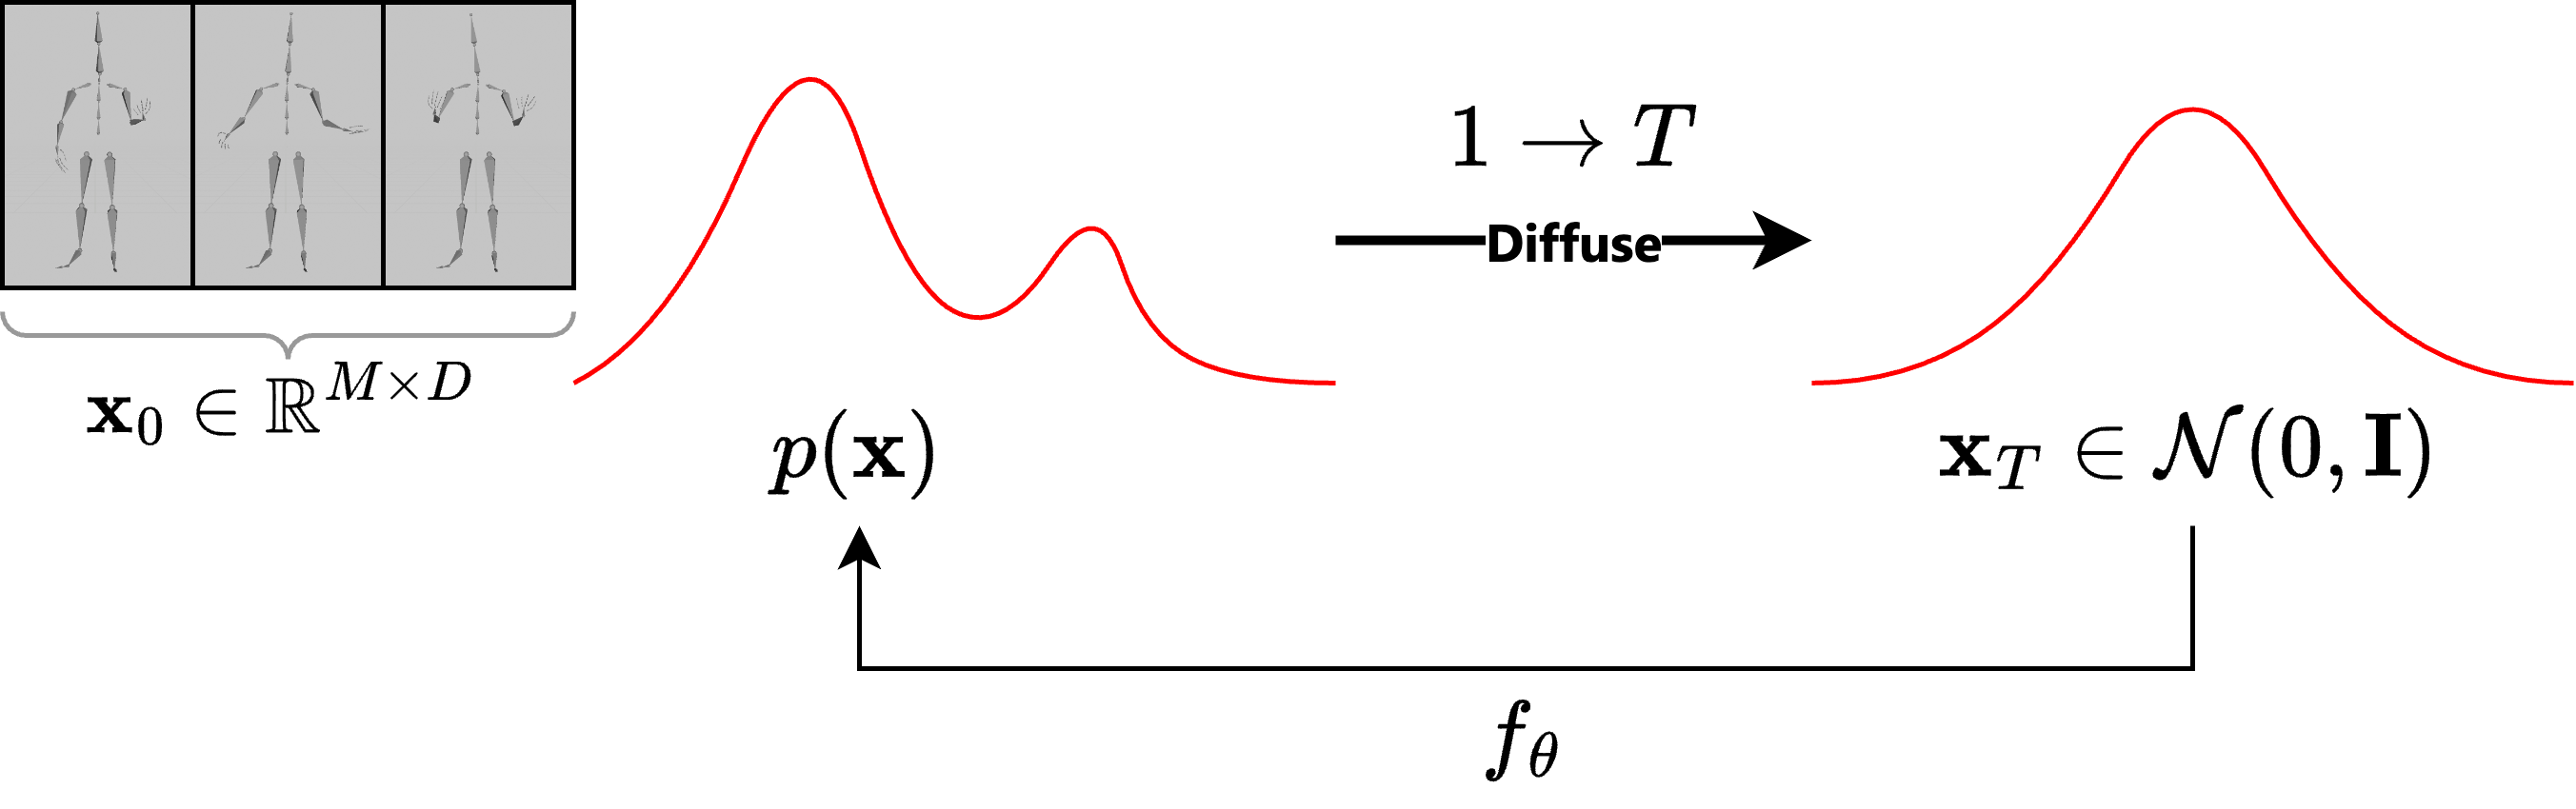
\includegraphics[width=0.8\textwidth]{DistributionTransition}
\end{figure}

\end{frame}

\begin{frame}{Ký hiệu}
	\textbf{Tham số}: Đang huấn luyện {\Large$\textcolor{cyan}{\theta}$}, đã huấn luyện xong: {\Large$\textcolor{cyan}{\theta}'$}, {\Large$\textcolor{cyan}{\hat{\bx}}$}: dự đoán
	\vspace{-5pt}
	
	\textbf{Phân phối chuẩn}
	\vspace{-5pt}
	{\Large $$\mathcal{N}(\textcolor{red}{a} \mathbf{x}, \textcolor{blue}{b^2})$$}
	\vspace{-15pt}
	\begin{itemize}
		\item Một hàm $f(x) = a x + b\epsilon$ với $\epsilon \in \mathcal{N}(0, \mathbf{1})$ được ký hiệu là $f(x) \sim \mathcal{N}(a x, b^2) $
		
		\item Trung bình: $\mu = \textcolor{red}{a}x=\frac{1}{n} \sum_{i=1}^{n} x_i$
		
		\item Phương sai: $\sigma^2 = \textcolor{blue} {b^2} = \frac{1}{n} \sum_{i=1}^{n} (x_i - \mu)^2$
		
	\end{itemize}
	\textbf{Xác xuất có điều kiện}
	\vspace{-5pt}
	{\Large $$p(\textcolor{green}{x}| \textcolor{orange}{y})$$}
	\vspace{-15pt}
	
	\begin{itemize}
		\item $p(\textcolor{green}{x}| \textcolor{orange}{y})$ là xác xuất có điều kiện.
		\item $\textcolor{orange}{y}$: xảy ra trước (bên phải)
		\item $\textcolor{green}{x}$: sảy ra sau y (bên trái)
	\end{itemize}

\end{frame}

\begin{frame}{Đặc điểm của việc học dữ liệu Motion}
	
	\begin{columns}
		\begin{column}{0.55\textwidth}
			\textbf{Quan hệ giữa dữ liệu cử chỉ và âm thanh}:
			\begin{itemize}
				\item Một đoạn cử có thể bao gồm nhiều âm thanh.
				\item Mỗi âm thanh có thể tương ứng với nhiều đoạn cử chỉ khác nhau.
			\end{itemize}
			%		Baseline: \textbf{MDM}  (Human Motion Diffusion Model)
			\textbf{Khó khăn}
			\begin{itemize}
				\item Dữ liệu ít, chi phí cao
				\item Thiếu nhãn và dữ liệu tương ứng giữa âm thanh, cử chỉ.
				\item Quá trình sinh có thể dể điều khiển 
				%			hơn GAN.
			\end{itemize}
			liệu
			%		\textit{Mô hình Diffusion}:
			%		\begin{itemize}
				%			\item Ít yêu cầu về dữ liệu gắn nhãn
				%			\item Khả năng tương tác và điều chỉnh dễ dàng
				%			\item Tính ổn định cao
				%		\end{itemize}
		\end{column}
		\begin{column}{0.45\textwidth}
			
			\begin{columns}
				\begin{column}{0.5\textwidth}
					\begin{figure}
						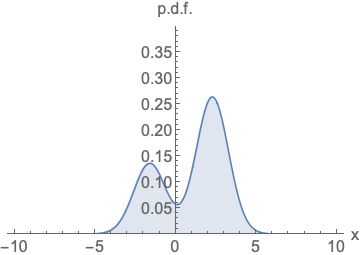
\includegraphics[width=\textwidth]{ProbabilityDensityFunctions.png}
						\caption{\scriptsize Phải chuẩn hoá (diện tích dưới đường cong phải tích phân thành một)}
					\end{figure}
				\end{column}
				\begin{column}{0.5\textwidth}
					\begin{figure}
						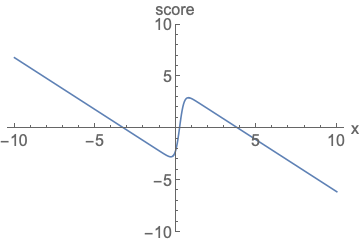
\includegraphics[width=\textwidth]{ScoreFunction.png}
						\caption{\scriptsize Không cần chuẩn hoá.}
					\end{figure}
				\end{column}
			\end{columns}
			
			
			
			\begin{columns}
				\begin{column}{0.5\textwidth}
					\centering
					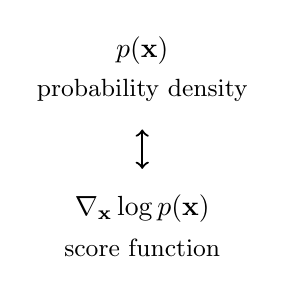
\begin{tikzpicture}
						\node at (0, 1) {$p(\mathbf{x})$};
						
						\node at (0, 0.5) {\small \text{probability density}};
						
						\draw[<->, thick] (0, 0) -- (0, -0.5);
						
						\node at (0, -1) {$\nabla_\mathbf{x} \log p(\mathbf{x})$};
						
						\node at (0, -1.5) {\small \text{score function}};
					\end{tikzpicture}
					
				\end{column}
				\begin{column}{0.5\textwidth}
					\begin{figure}
						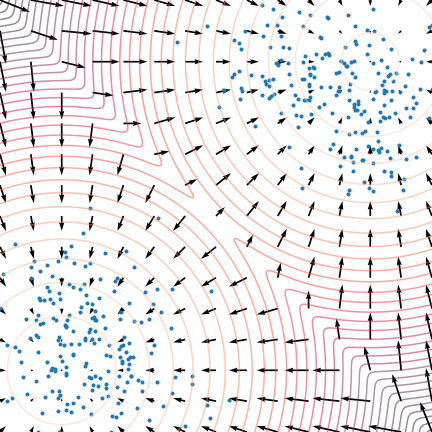
\includegraphics[width=\textwidth]{CompareScoreFunction.png}
						\caption{\scriptsize score function vs probability density}
					\end{figure}
				\end{column}
			\end{columns}
		\end{column}
	\end{columns}	
\end{frame}


\begin{frame}{Diffuse và Denoise thông thường}
%\begin{columns}
%	\begin{column}[T]{0.5\textwidth}
%	
%	\end{column}
%	
%	\hspace*{-1em}
%	
%	\begin{column}[T]{0.5\textwidth}
%		
%	\end{column}
%\end{columns}

\textbf{Diffuse}: Cho $\{\alpha_t \in (0, 1)\}_{t=1}^T$ và $\alpha_1 > \alpha_2 > \dots > \alpha_T$.

Với nhiễu:  $\boldsymbol{\epsilon}_{0}, \boldsymbol{\epsilon}_{1}, \dots \boldsymbol{\epsilon}_{T} \sim \mathcal{N}(\mathbf{0}, \mathbf{I});$
$\boldsymbol{\epsilon}_i \neq \boldsymbol{\epsilon}_j \ (\forall i, j \in T) $, nhiễu $\epsilon_t$ cố định.
\vspace{-25pt}

\begin{equation}
	\mathbf{x}_t=\sqrt{\alpha_t} \cdot \mathbf{x}_{t-1}+\sqrt{1 - \alpha_t} \cdot \epsilon
\end{equation}
\vspace{-15pt}

%	\[
%	q(x_t | x_{t-1}) = \mathcal{N}(x_t; \sqrt{1 - \beta_t} \, x_{t-1}, \beta_t \, I)
%	\]
\begin{figure}
	\centering
	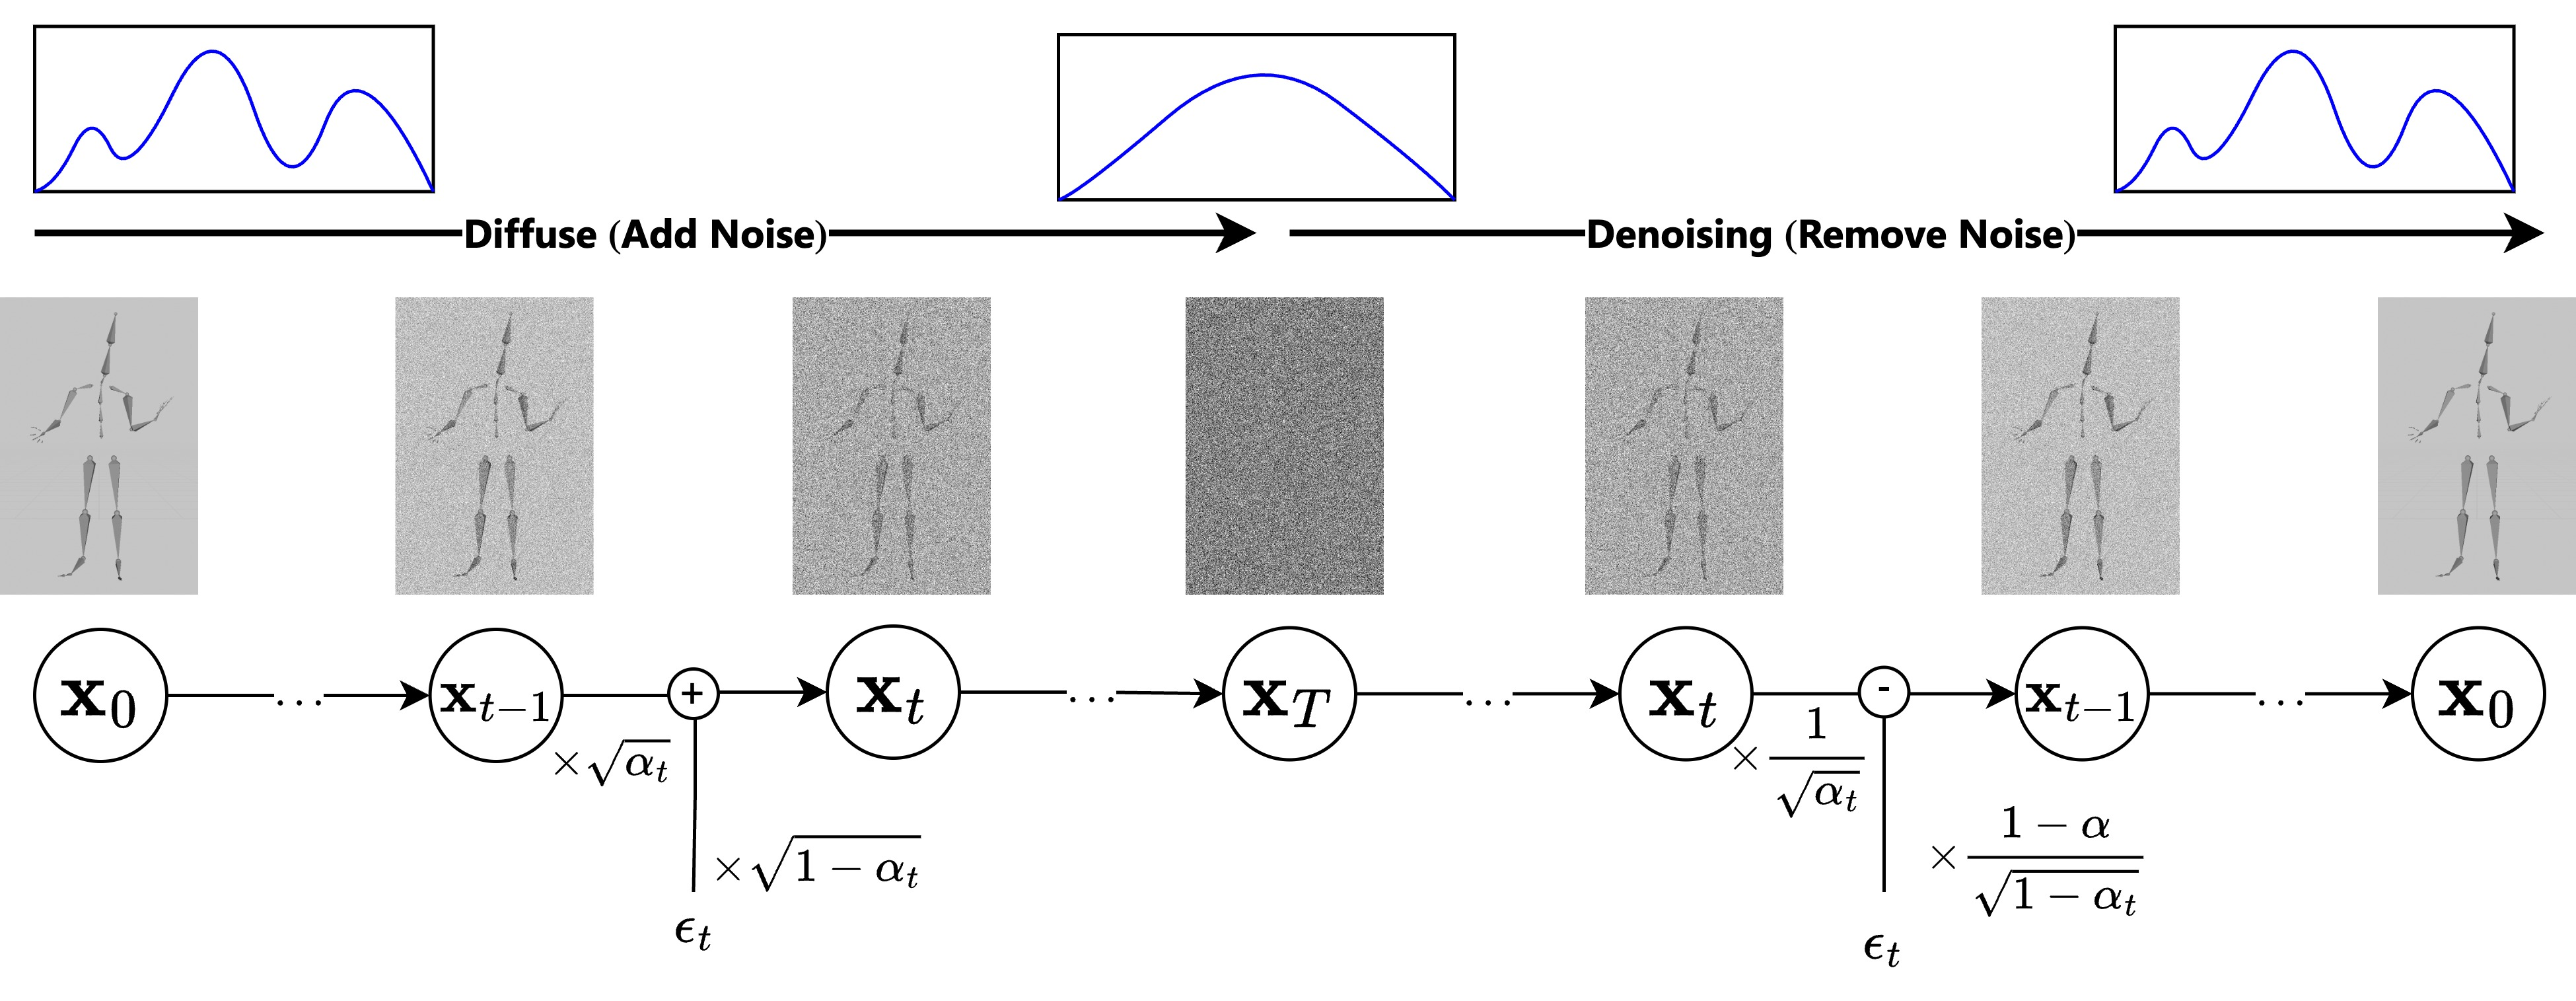
\includegraphics[width=\textwidth]{DiffuseAndDenoise.jpg}
\end{figure}
%\begin{equation}
%	\mathbf{x}_{t-1}=\frac{1}{\sqrt{\alpha_t}}\left(\bx_t-\sqrt{1 - \alpha_t} \cdot \epsilon (\mathbf{x}_t, t )\right)
%\end{equation}

\begin{columns}
	\begin{column}{0.5\textwidth}
		\textbf{Denoise}
		\begin{equation}
			\mathbf{x}_{t-1} = \frac{1}{\sqrt{\alpha_{t}}} (\mathbf{x}_t - \sqrt{1- \alpha_t} \cdot \epsilon)
		\end{equation}
	\end{column}
	\begin{column}{0.5\textwidth}
	\begin{figure}
		\centering
		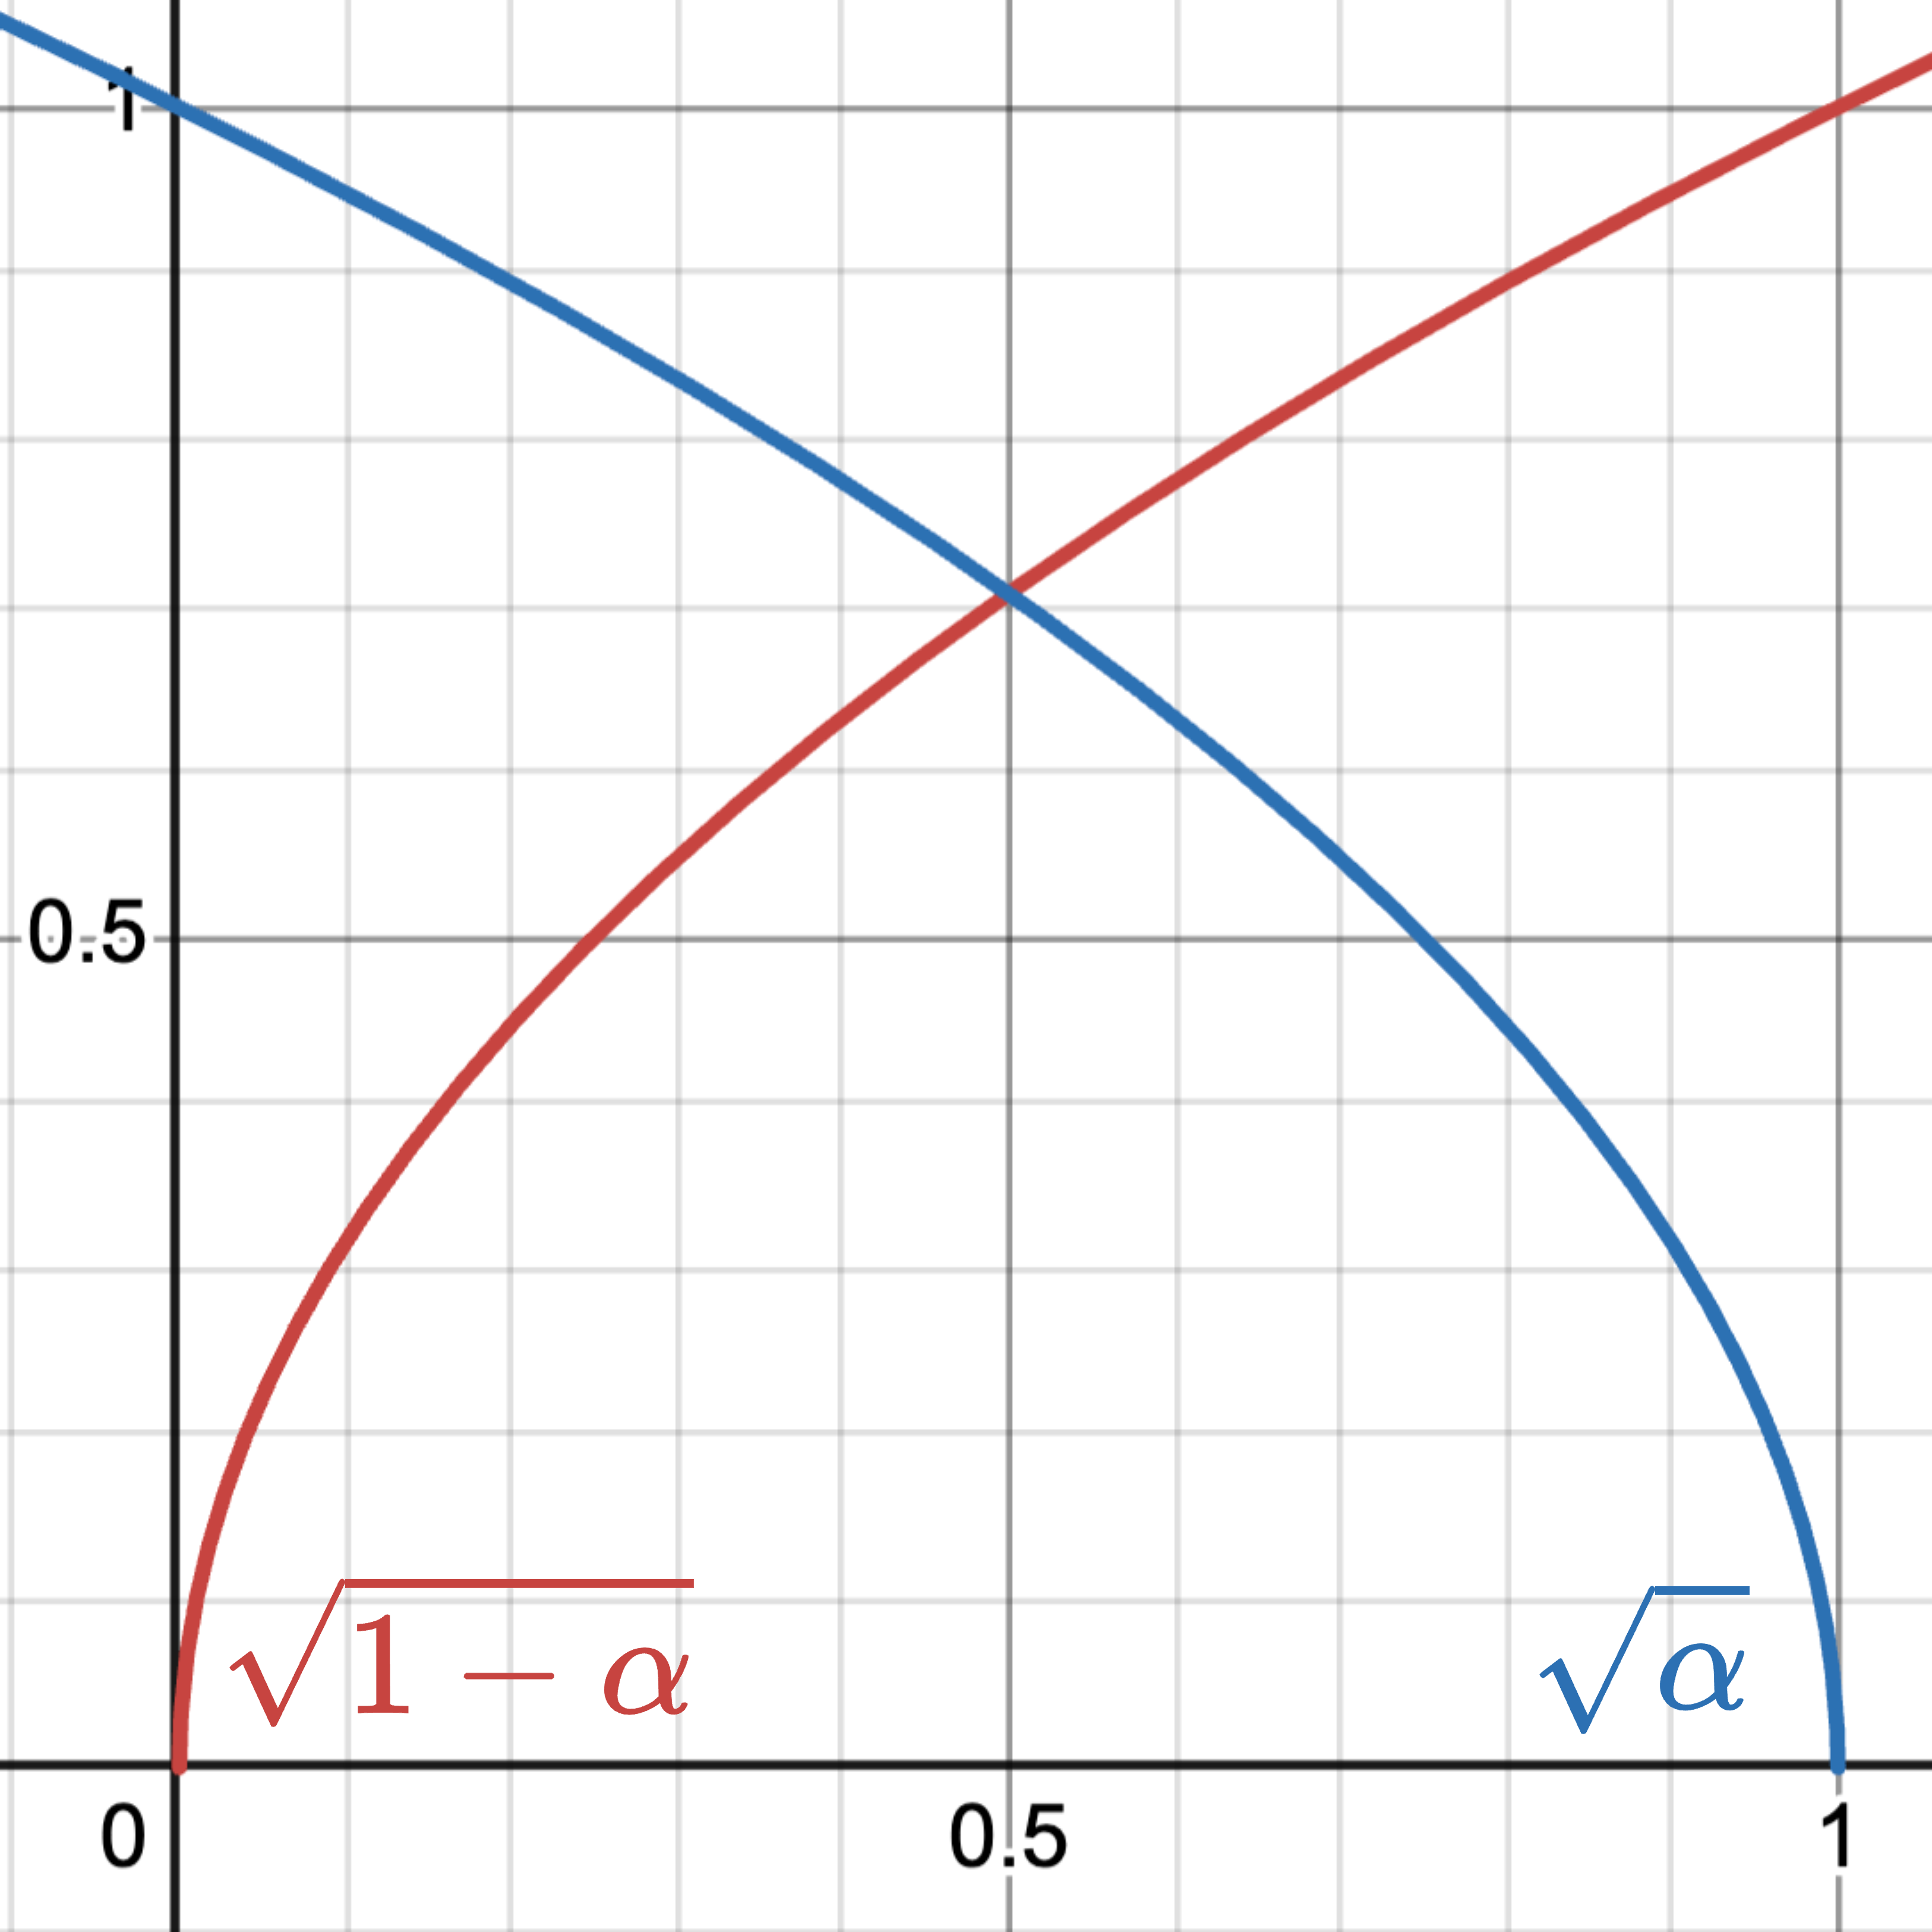
\includegraphics[width=0.4\textwidth]{SquareAlpha.png}
	\end{figure}
	\end{column}
\end{columns}

\end{frame}


\begin{frame}{Quan hệ $\bx_t$ và $\bx_{t - 1}$}
	
	Ta có thể suy ra $\bx_t$ từ $\bx_0$ và ngược lại. Với $ \boldsymbol{\epsilon}_{t-1}, \boldsymbol{\epsilon}_{t-2}, \dots \sim \mathcal{N}(\mathbf{0}, \mathbf{I})$
	%\begin{align*}
	%	\mathbf{x}_t & = \sqrt{\alpha_t}\mathbf{x}_{t-1} + \sqrt{1 - \alpha_t} \boldsymbol{\epsilon}_{t-1} \\
	%	& = \sqrt{\alpha_t \alpha_{t-1}} \mathbf{x}_{t-2} + \sqrt{1 - \alpha_t \alpha_{t-1}} \bar{\boldsymbol{\epsilon}}_{t-2} \\
	%	& = \dots \\
	%	& = \sqrt{\bar{\alpha}_t}\mathbf{x}_0 + \sqrt{1 - \bar{\alpha}_t}\boldsymbol{\epsilon}
	%\end{align*}
	\vspace{-10pt}
	
	\begin{figure}
		\centering
		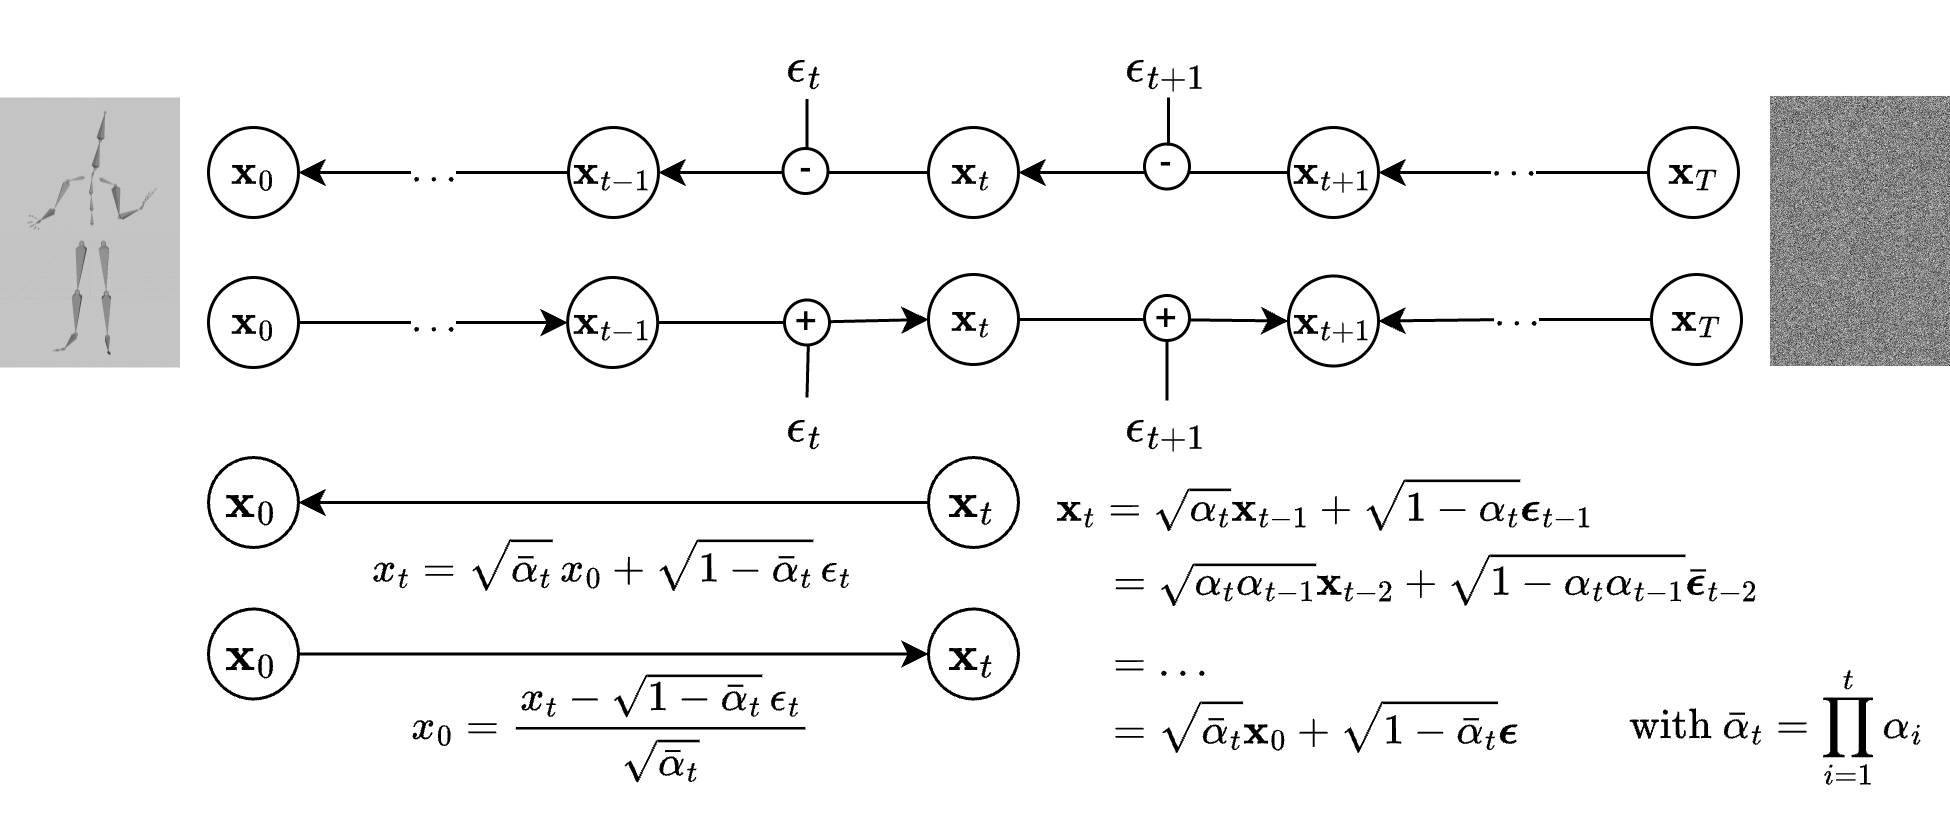
\includegraphics[width=\textwidth]{XRelation.png}
	\end{figure}
	%\vspace{-10pt}
	%	\mathbf{x}_t = \sqrt{\bar{\alpha}_t}\mathbf{x}_0 + \sqrt{1 - \bar{\alpha}_t}\boldsymbol{\epsilon}
	\begin{columns}
		\begin{column}{0.5\textwidth}
			\begin{itemize}
				\item $\bar{\alpha}_1 > \dots > \bar{\alpha}_T$
				\item Tổng hai nhiễu cũng là nhiễu:
				\footnotesize
				$$
				\mathcal{N}(\mathbf{0}, \sigma_1^2\mathbf{I}) + 
				\mathcal{N}(\mathbf{0}, \sigma_2^2\mathbf{I})
				=\mathcal{N}(\mathbf{0}, (\sigma_1^2 + \sigma_2^2)\mathbf{I})
				$$
			\end{itemize}
		\end{column}
		\begin{column}{0.5\textwidth}
			
			\begin{figure}
				\centering
				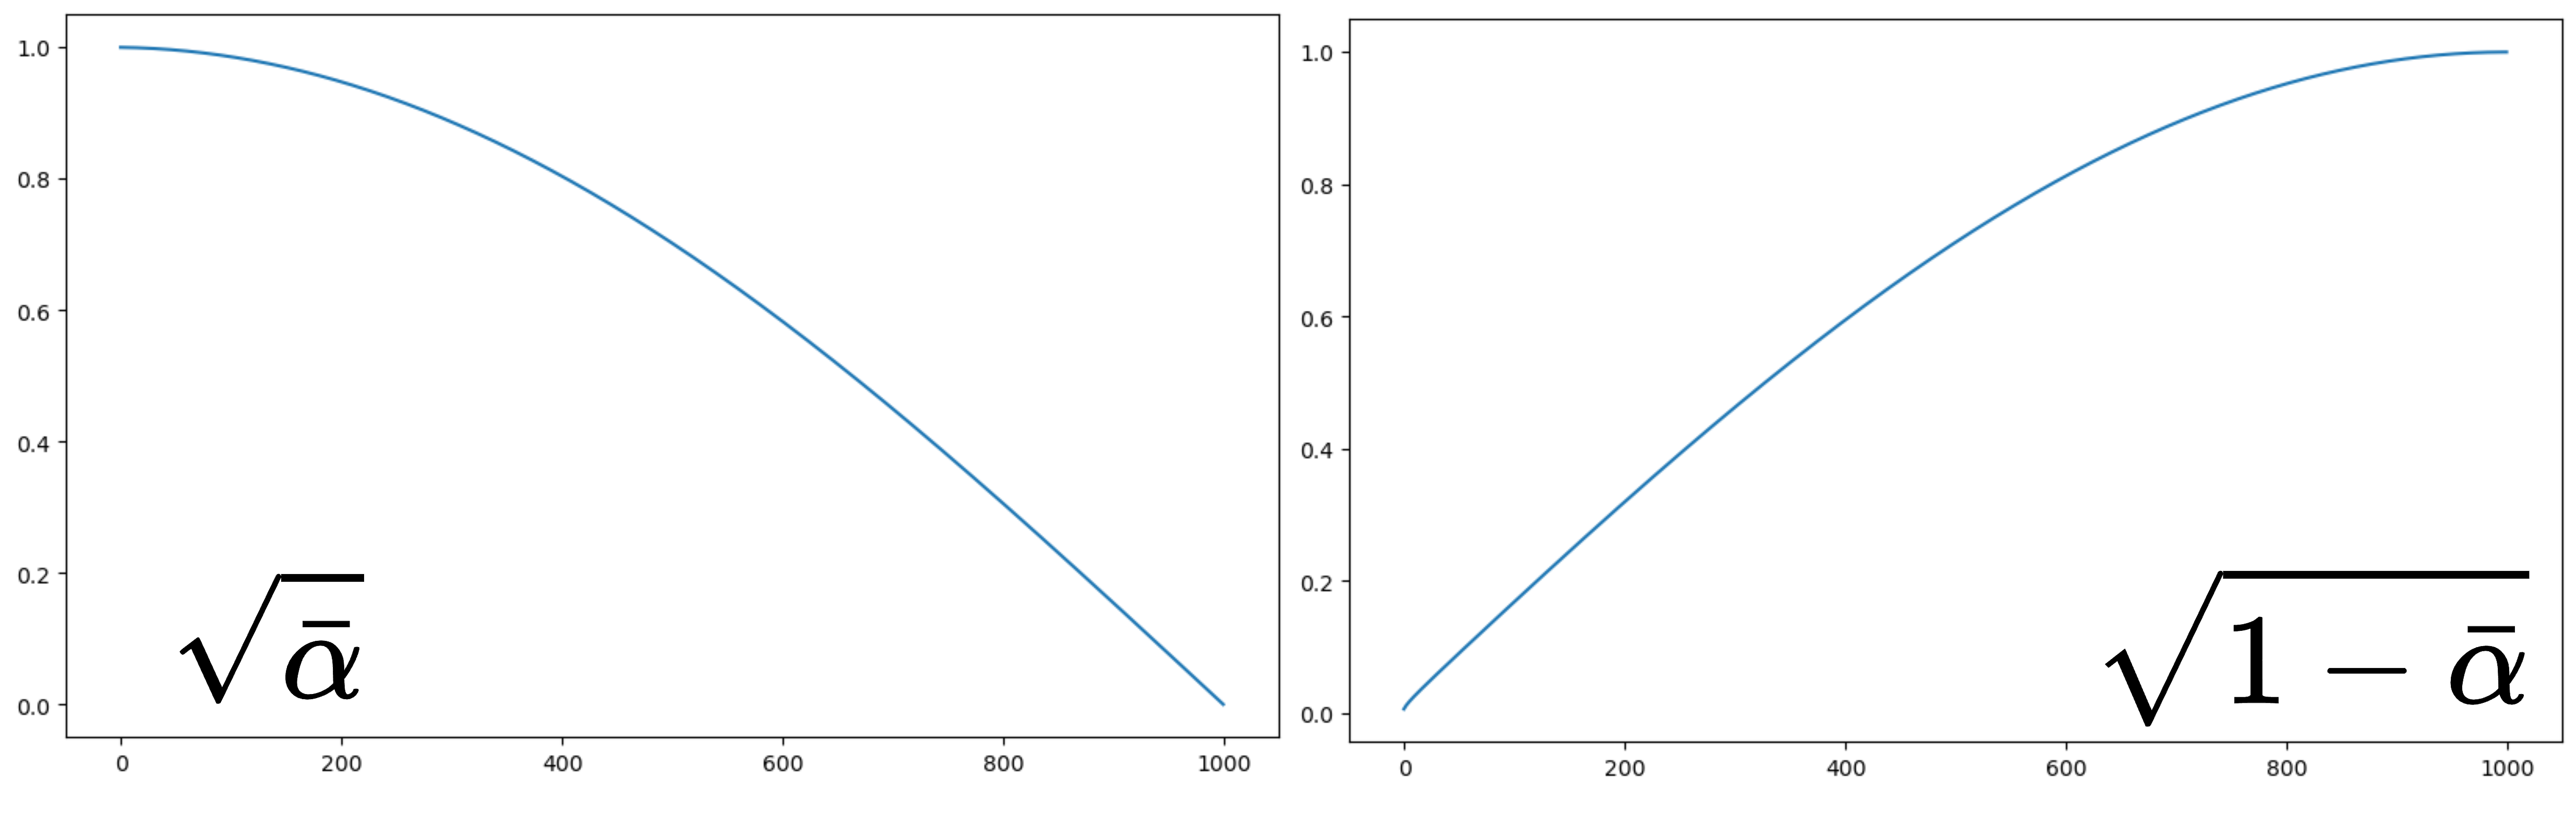
\includegraphics[width=\textwidth]{AlphaCumprod}
			\end{figure}
			
			
		\end{column}
	\end{columns}
	
\end{frame}


\begin{frame}{$q(\bx_t | \bx_{t-1})$ và $p_{\theta}(\bx_{t-1} | \bx_t ) $  trong DDPM }
	\textbf{DDPM} (Denoising Diffusion Probabilistic Model)
\begin{figure}
	\centering
	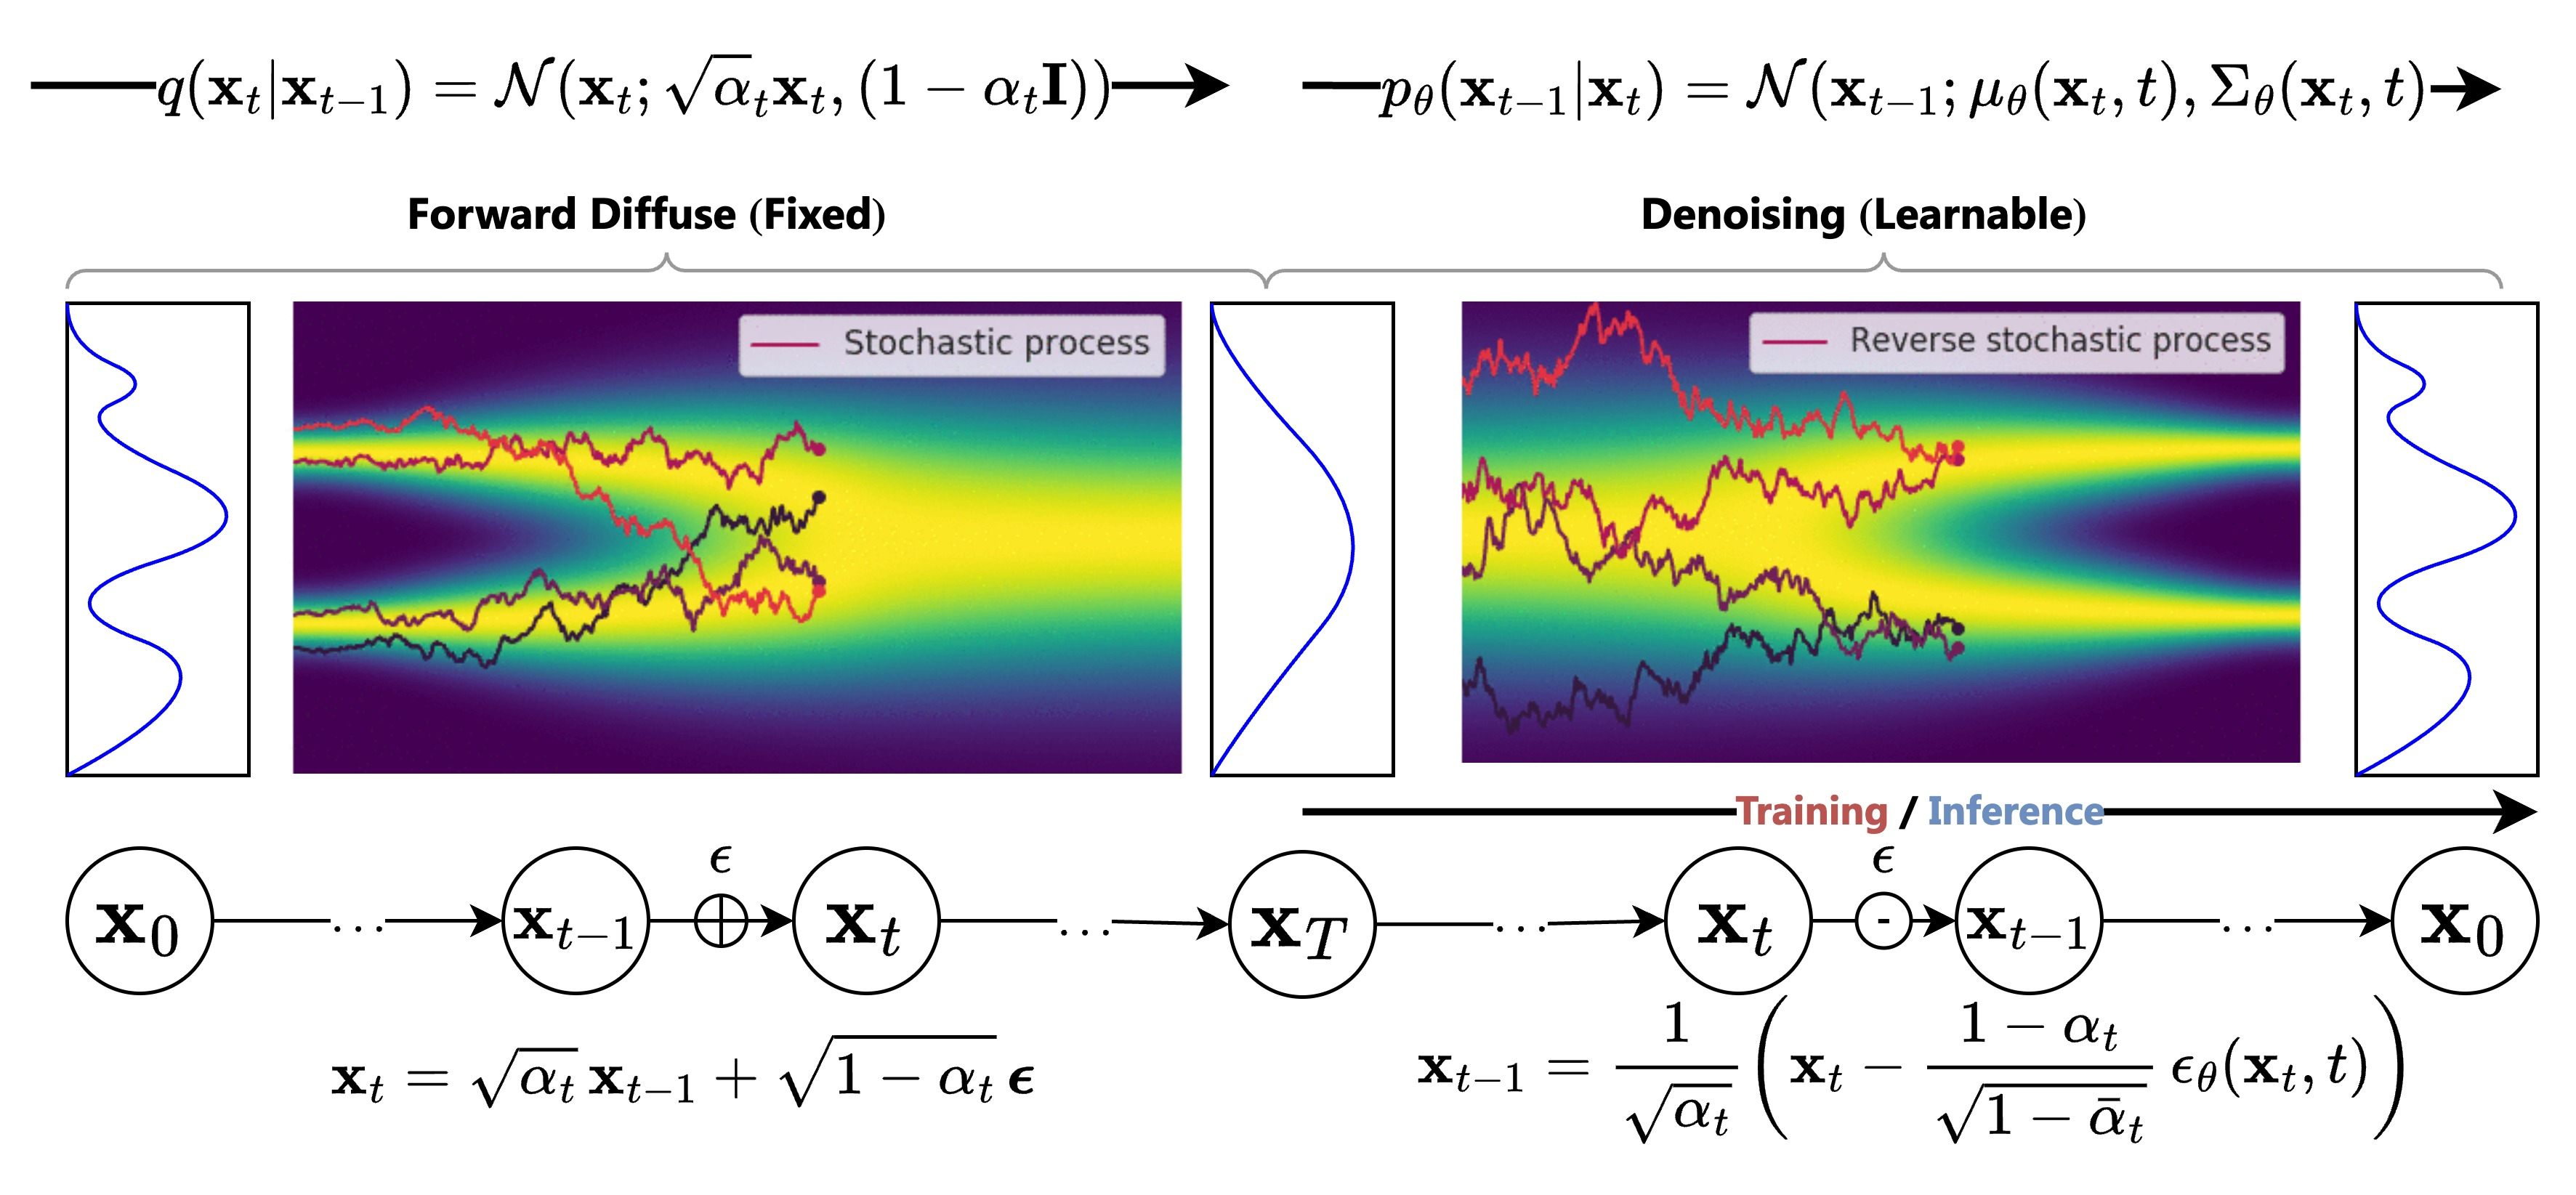
\includegraphics[width=\textwidth]{PQ}
\end{figure}
	
\begin{itemize}
	\item $q (\mathbf{x}_{t} | \mathbf{x}_{t-1}) = \mathcal{N}(\mathbf{x}_t; \sqrt{\alpha}_t \mathbf{x}_t, (1 - \alpha_t \mathbf{I}))$
	\item $p_\theta (\mathbf{x}_{t-1} | \mathbf{x}_{t}) = \mathcal{N}(\mathbf{x}_{t-1}; \mu_\theta{(\mathbf{x}_t, t)}, {\Sigma}_{\theta} {  (\mathbf{x}_t, t ) }$
\end{itemize}
%	$q(\mathbf{x}_t \vert \mathbf{x}_0) = \mathcal{N}(\mathbf{x}_t; \sqrt{\bar{\alpha}_t} \mathbf{x}_0, (1 - \bar{\alpha}_t)\mathbf{I})$
%
%
%
%\begin{equation}
%	\mathbf{x}_{t-1}=\frac{1}{\sqrt{1- \beta_t}}\left(\bx_t-\sqrt{\beta_t} \cdot \epsilon_{\color{red}{\theta}}\left(\mathbf{x}_t, t\right)\right)+\color{red}{\beta_t \cdot \sigma_t \mathbf{z}} \color{black}{}
%\end{equation}

\end{frame}

\begin{frame}{Vanilla Diffusion với $\epsilon$ Objective}
	\begin{figure}
		\centering
		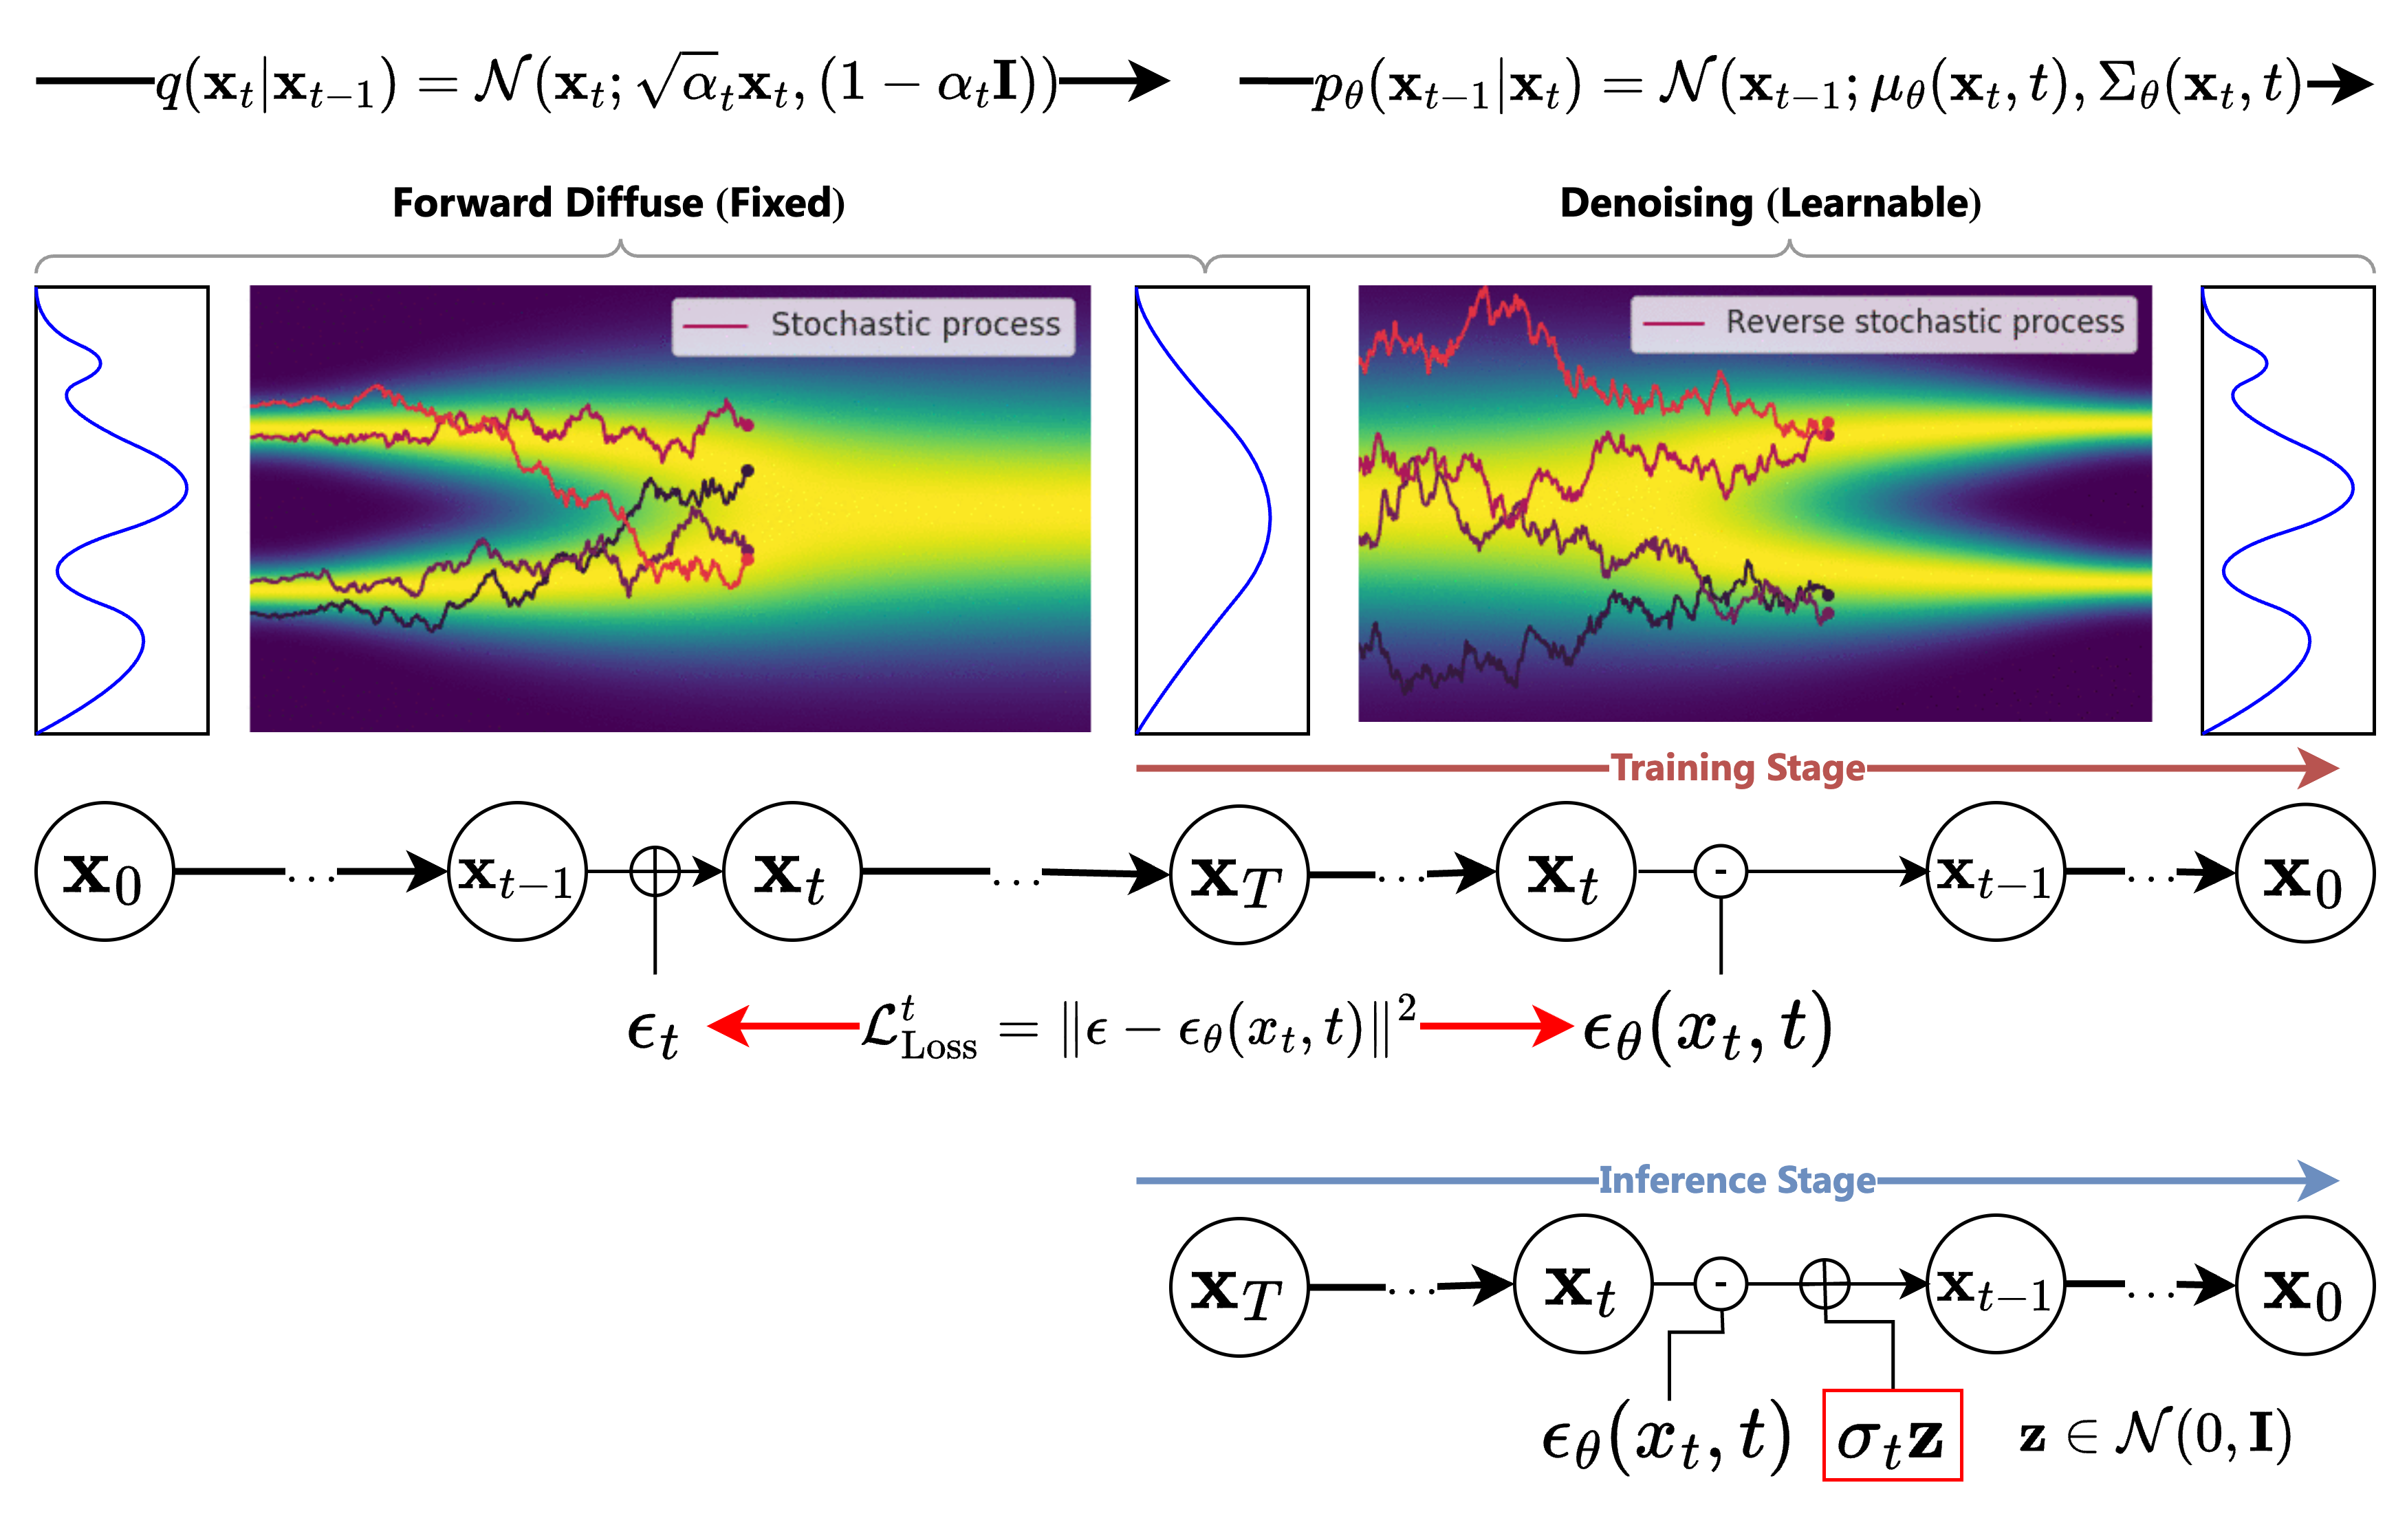
\includegraphics[width=0.95\textwidth]{TrainingAndSamplingStandard.png}
	\end{figure}
\end{frame}

\begin{frame}{Điều khiển $\sigma_t$ bằng với Langevin dynamics}
%	Cho $L$ là biến điều chỉnh độ lệch chuẩn
	%	 $\mathcal{N}(0, \sigma_i^2 I), i=1,2,\cdots,L$. $\mathbf{s}_\theta(\mathbf{x}, i) \approx \nabla_\mathbf{x} \log p_{\sigma_i}(\mathbf{x})$ $i= 1, 2, \cdots, L$.
	
%	Ta dễ dàng sinh mẫu (sampling) từ ${\sigma_i}(\mathbf{x})$ bằng cách lấy mẫu $\mathbf{x} \sim p(\mathbf{x})$  và tính $\mathbf{x} + \sigma_i \mathbf{z}$ với $\mathbf{z} \sim \mathcal{N}(0, I)$
Trong quá trình Denoise ($T \rightarrow 0$)  $\sigma_T > \cdots  >  \sigma_2 > \sigma_1$, ta sẽ giảm $\sigma_t$ để giảm dần nhiễu, để mô hình có thể hội tụ ở những vùng có mật độ xác xuất cao.
	\begin{figure}
		\centering
		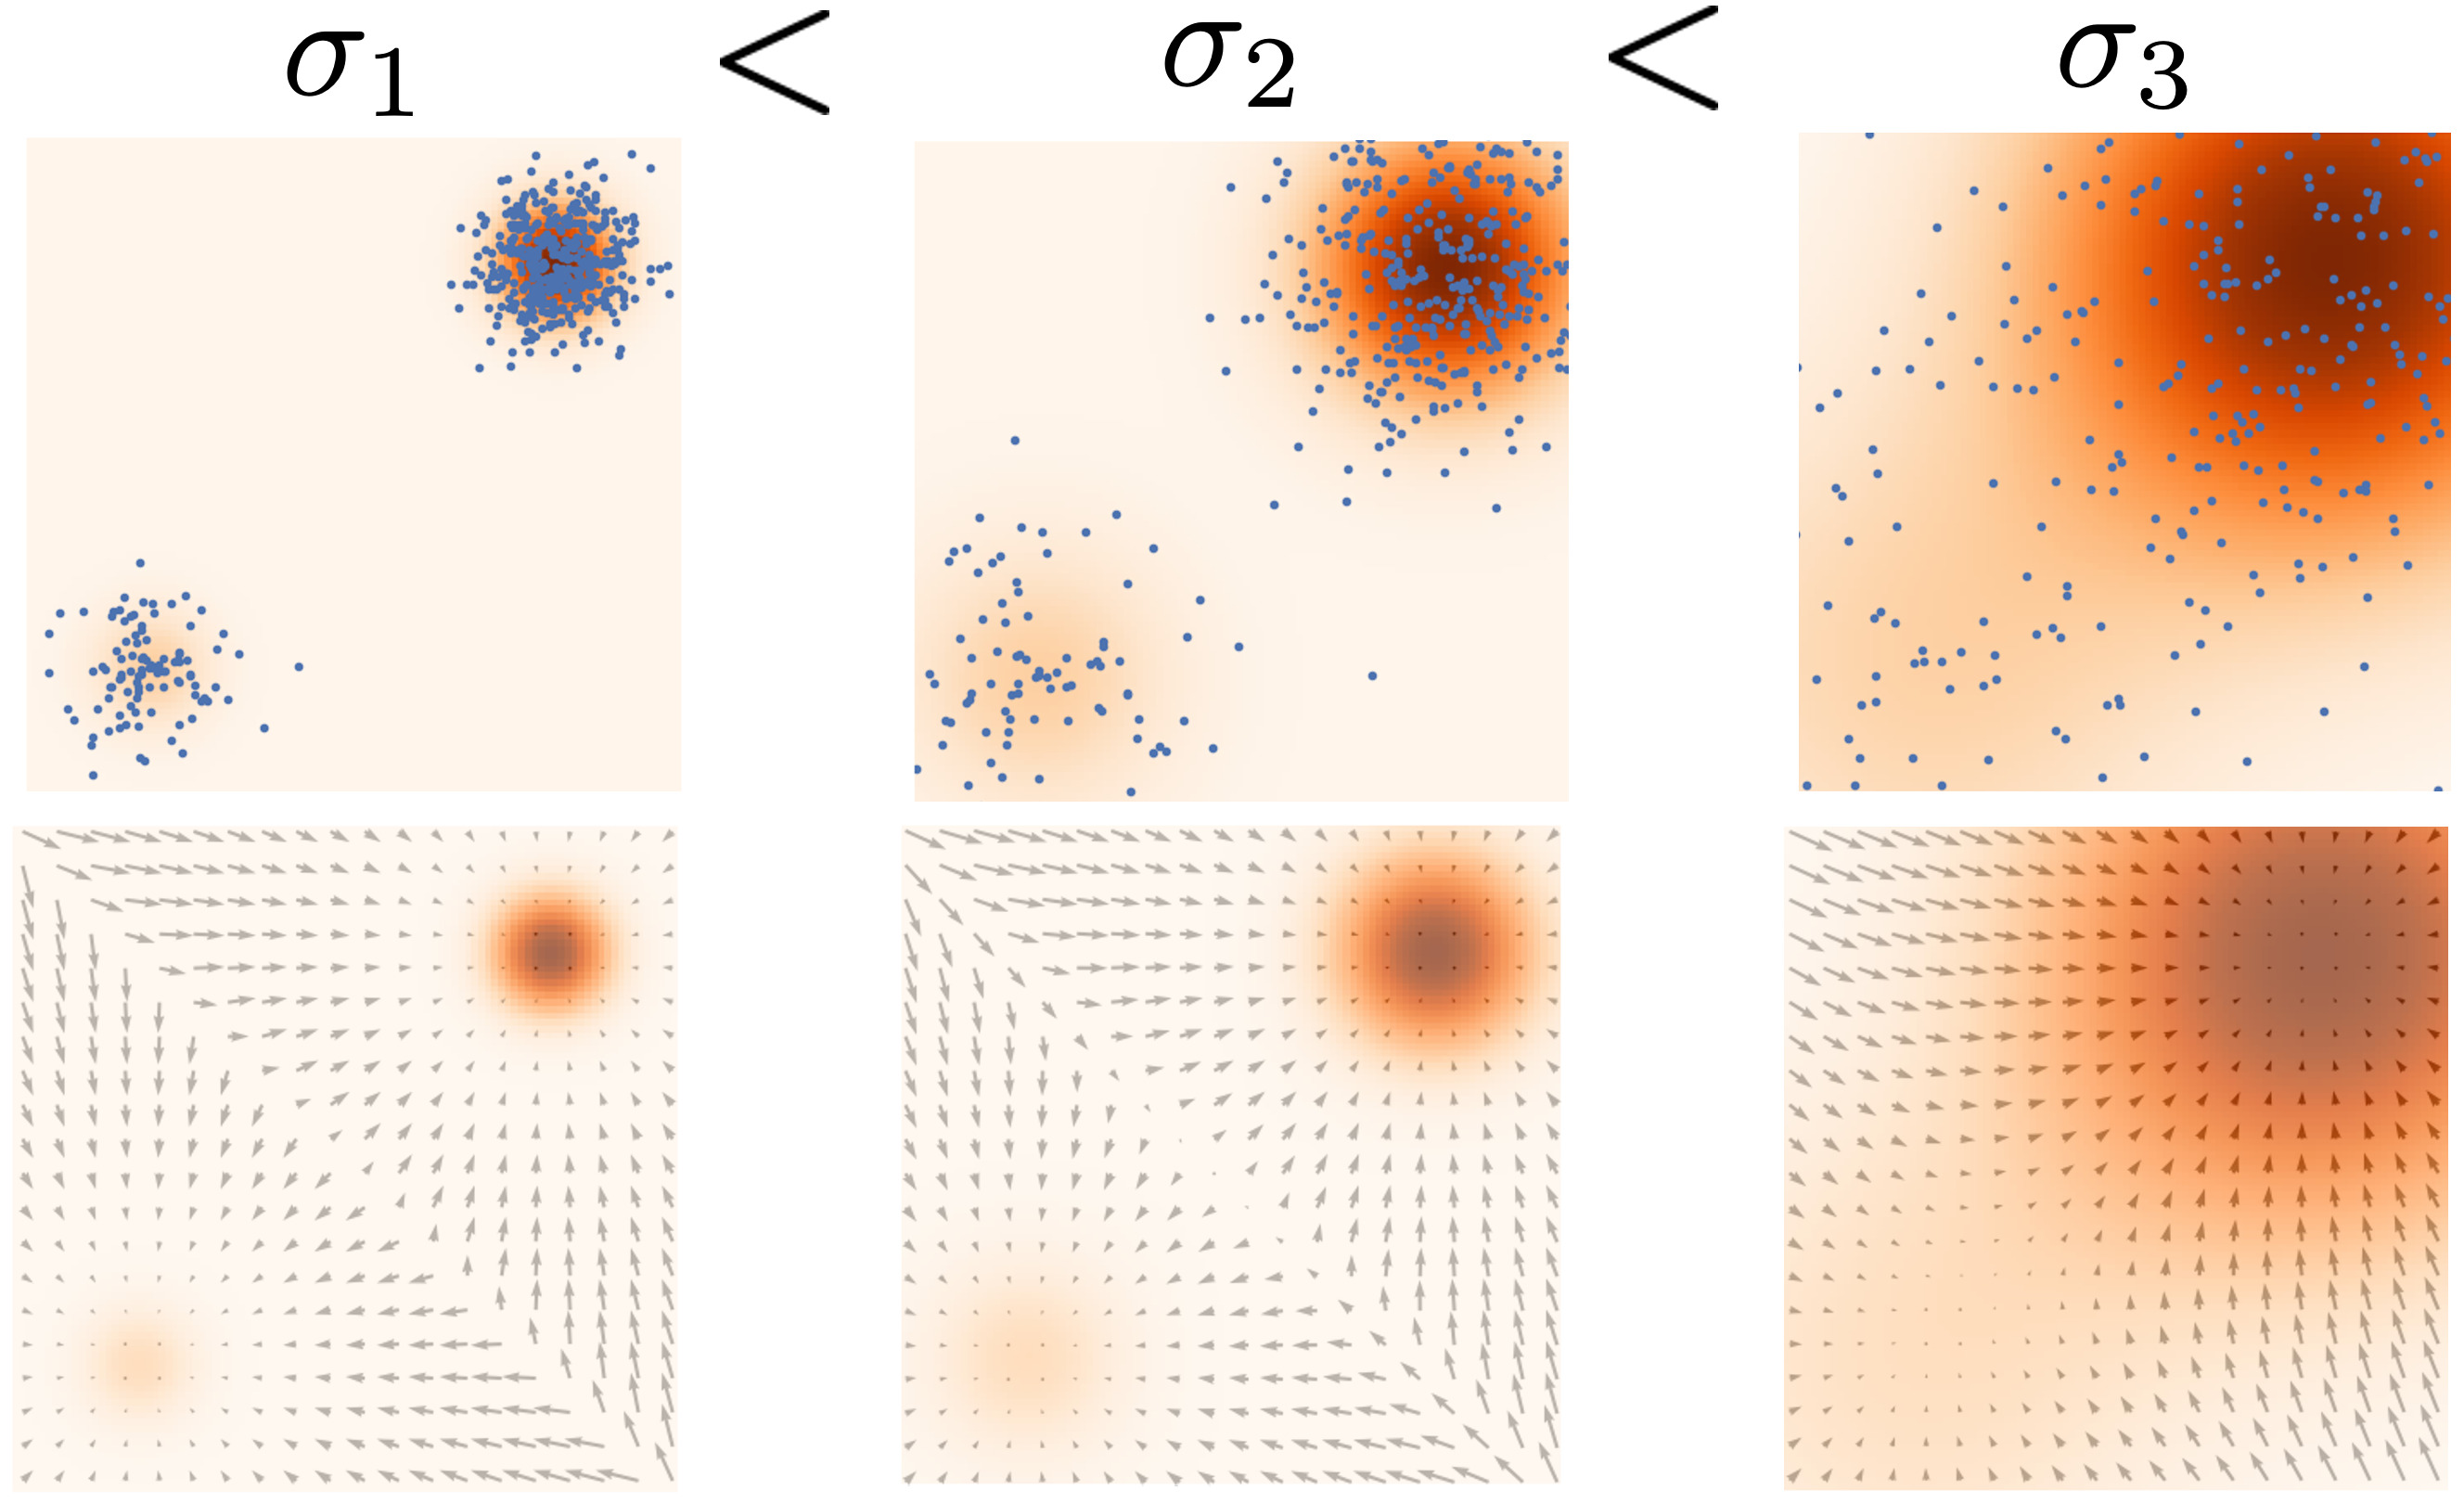
\includegraphics[width=0.8\linewidth]{NoiseScale.jpg}
	\end{figure}
\end{frame}

\begin{frame}{Training DDPM}
	\textbf{Hàm loss}: $\mathcal{L} = \sum_{t=1}^{T} \mathcal{L}_t$. $\mathcal{L}_{t}= \mathbb{E}_{\mathbf{x}_{0}, \epsilon_t \sim \mathcal{N}(0, I), t} \left[ \| \epsilon_t - \epsilon_\theta(\mathbf{x}_t, t) \|^2 \right]$
	
	\begin{figure}
		\centering
		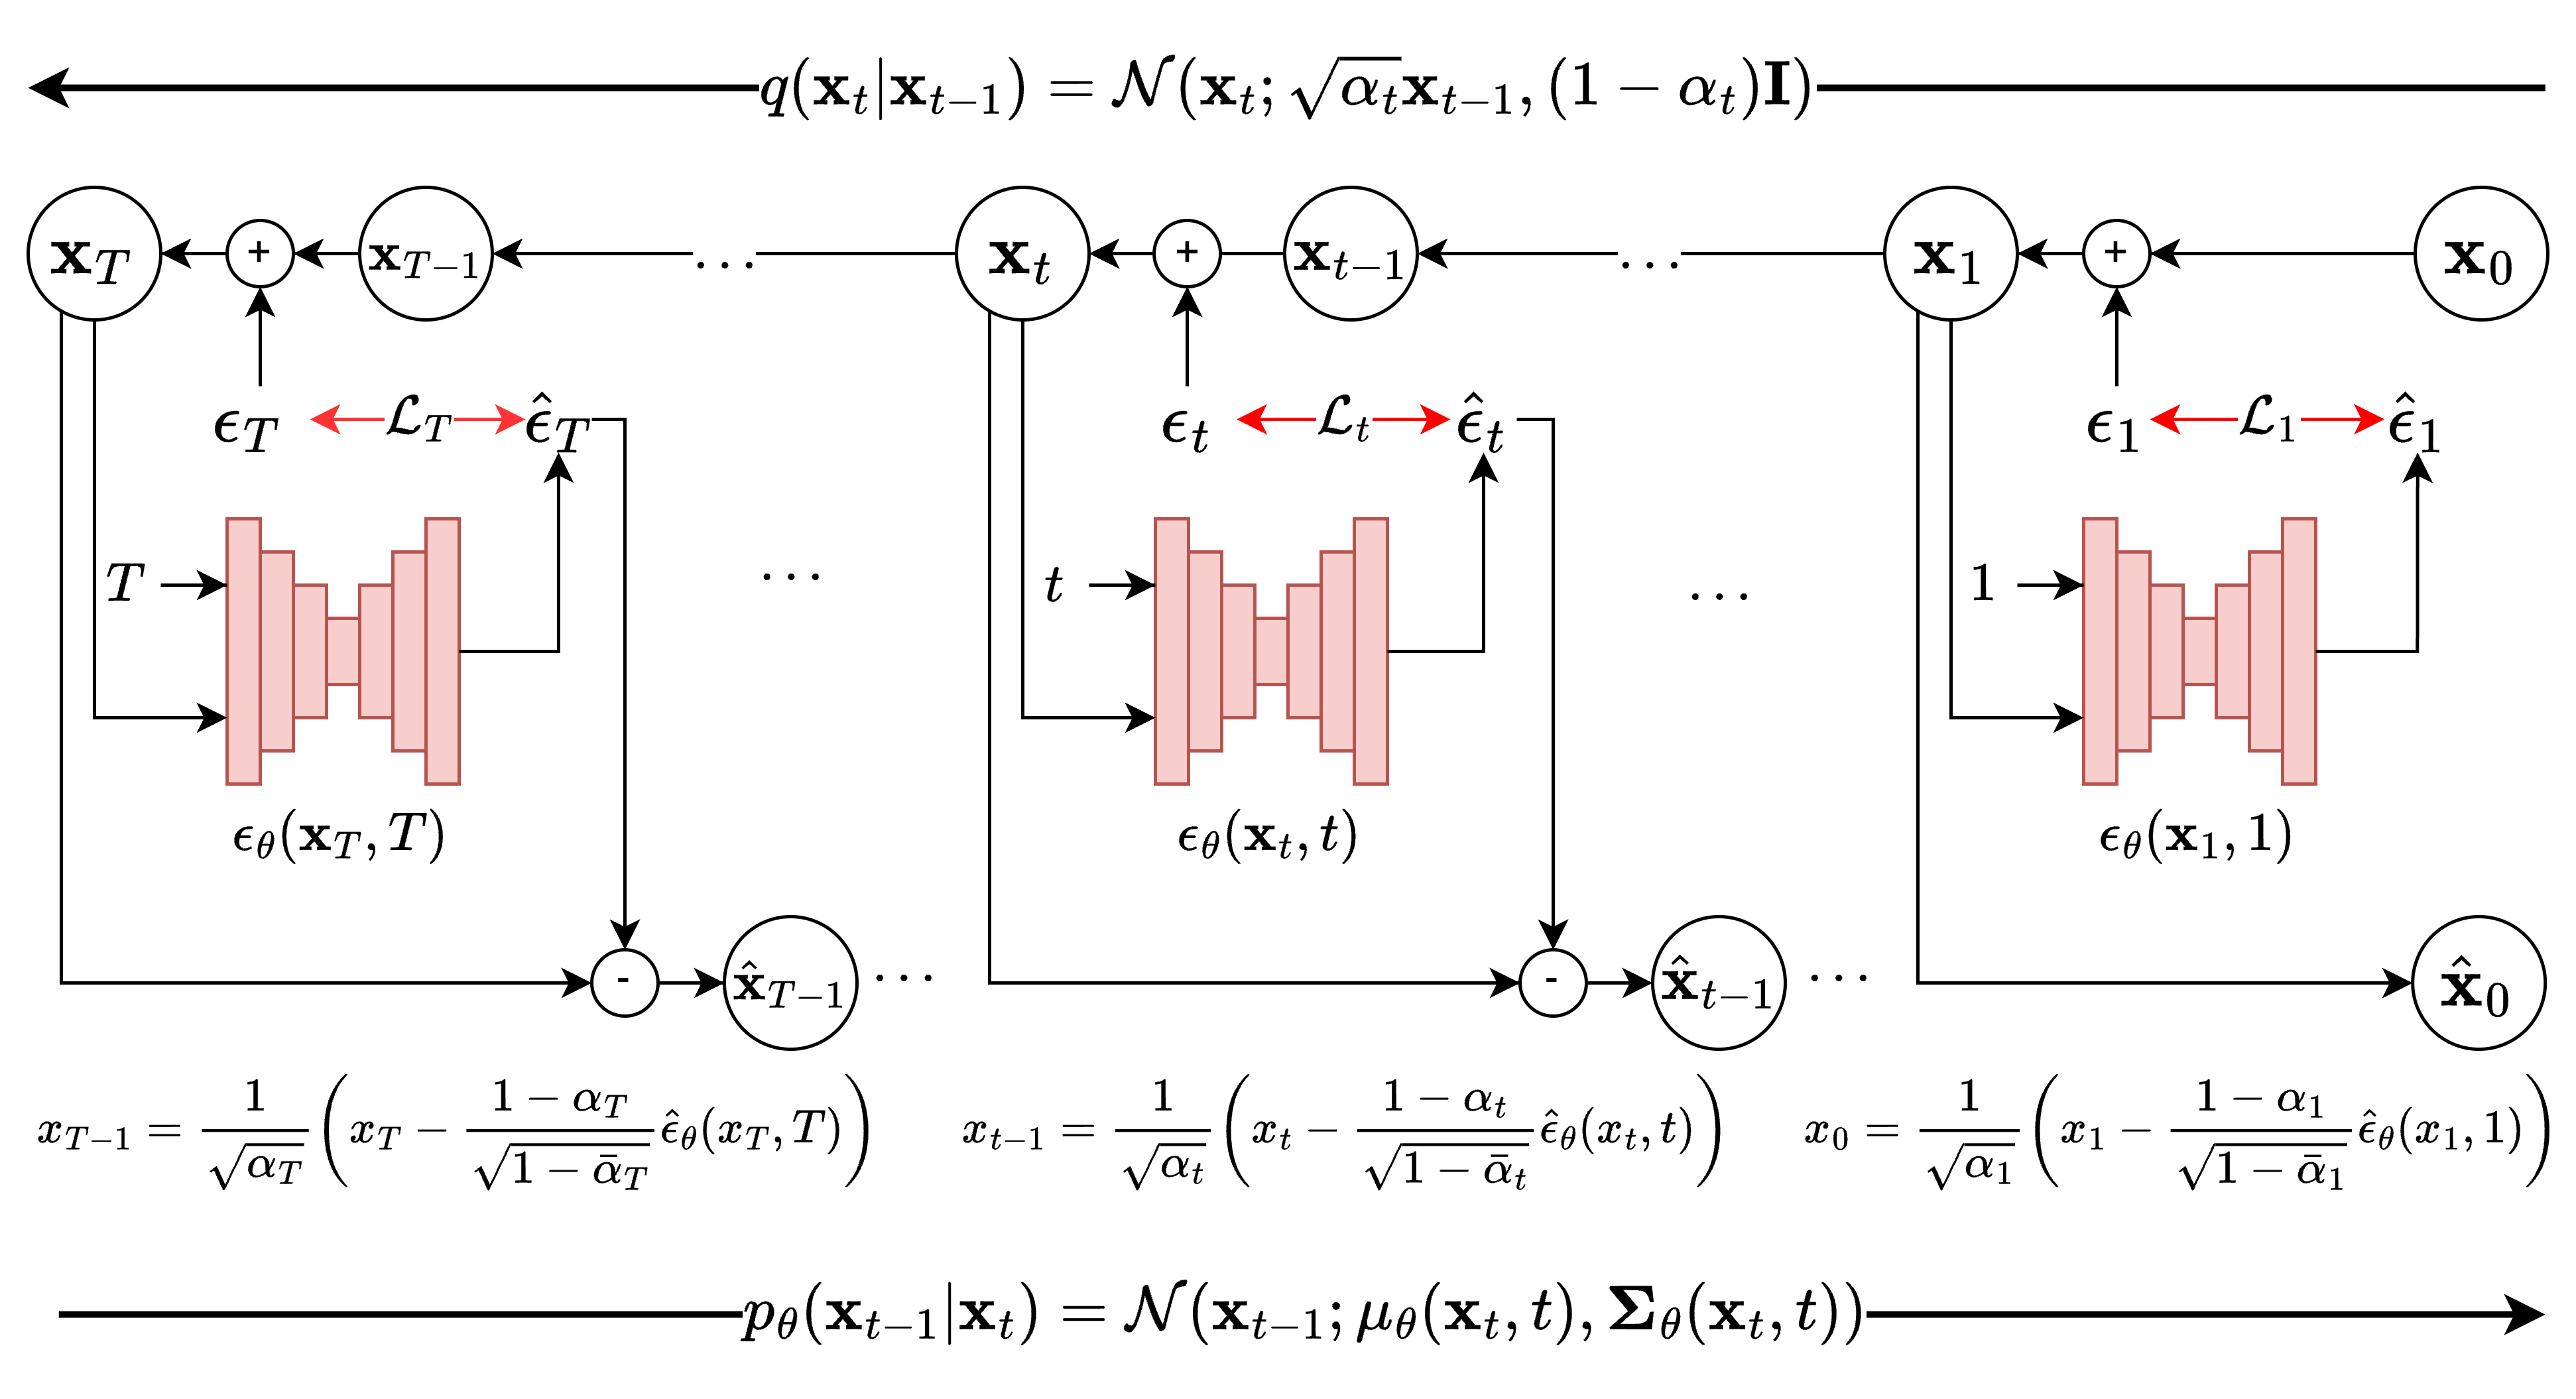
\includegraphics[width=\linewidth]{DDPMTraining}
	\end{figure}
\end{frame}

\begin{frame}{Các bước huấn luyện với DDPM}
	
	\begin{enumerate}
		\item Tính sẵn các giá trị $\sqrt{\alpha_t}$ $\sqrt{1 - \alpha_t}$ và $\sqrt{\bar{\alpha}_t}$ ở mọi bước $t: 1 \rightarrow T$.
		$\{\alpha_t \in (0, 1)\}_{t=1}^T$, $\alpha_1 < \alpha_2 < \dots < \alpha_T$
		\item Lấy nhãn $\bx_0$ từ phân bố của dữ liệu đã chuẩn hoá
		\item Random nhiễu $\bepsilon_t$ ở mọi bước $t: 1 \rightarrow T$, với  $\forall t:  \bepsilon_t \sim\mathcal{N}(\bzero,\bI)$
		\item Gây nhiễu (forward) $\bx_0$ để thu được $\bx_t$ ở mọi bước $t: 1 \rightarrow T$
		$$
		\mathbf{x}_t = \sqrt{\bar{\alpha}_t}\mathbf{x}_0 + \sqrt{1 - \bar{\alpha}_t}\boldsymbol{\epsilon}_t
		$$
		\item $\text{for all}$ $t$, lẫy $t$ \textbf{ngẫu nhiên} $t \sim [1, T]$
		\item Cho $\bx_t$ và $t$ vào mô hình để dự đoán nhiễu $\hat{\bepsilon} = \bepsilon_\theta(\mathbf{x}_t, t)$
		\item Đạo hàm để cập nhật trọng số $\qquad \grad_{\theta_t} \left\| \bepsilon_t - \bepsilon_\theta(\mathbf{x}_t, t) \right\|^2$
		$$
			\mathcal{L}_t = \mathbb{E}_{t \sim [1, T], \mathbf{x}_0, \boldsymbol{\epsilon}_t} \Big[\|\boldsymbol{\epsilon}_t - \boldsymbol{\epsilon}_\theta(\sqrt{\bar{\alpha}_t}\mathbf{x}_0 + \sqrt{1 - \bar{\alpha}_t}\boldsymbol{\epsilon}_t, t)\|^2 \Big]
		$$
		\item Quay lại bước 6 cho đến khi hội tụ để thu được $\theta'$
	\end{enumerate}
\end{frame}

\begin{frame}{Sampling DDPM}
	\textbf{Hàm sampling}:
	\begin{itemize}
		\item $\bx_T \in \mathcal{N}(0, \mathbf{I})$
	\end{itemize}
	
	\begin{equation*}
		x_{t-1} = \frac{1}{\sqrt{\alpha_t}} \left( x_t - \frac{1 - \alpha_t}{\sqrt{1 - \bar{\alpha}_t}} \hat{\epsilon}_{\theta'}(x_t, t) \right) + \sigma_t \mathbf{z}
	\end{equation*}
	
	\begin{itemize}
		\item Diffusion: $\mathcal{L}_{\text{loss}}= \mathbb{E}_{\mathbf{x}_{0}, \epsilon_t \sim \mathcal{N}(0, I), t} \left[ \| \epsilon_t - \epsilon_\theta(\mathbf{x}_t, t) \|^2 \right]$
	\end{itemize}
	\begin{figure}
		\centering
		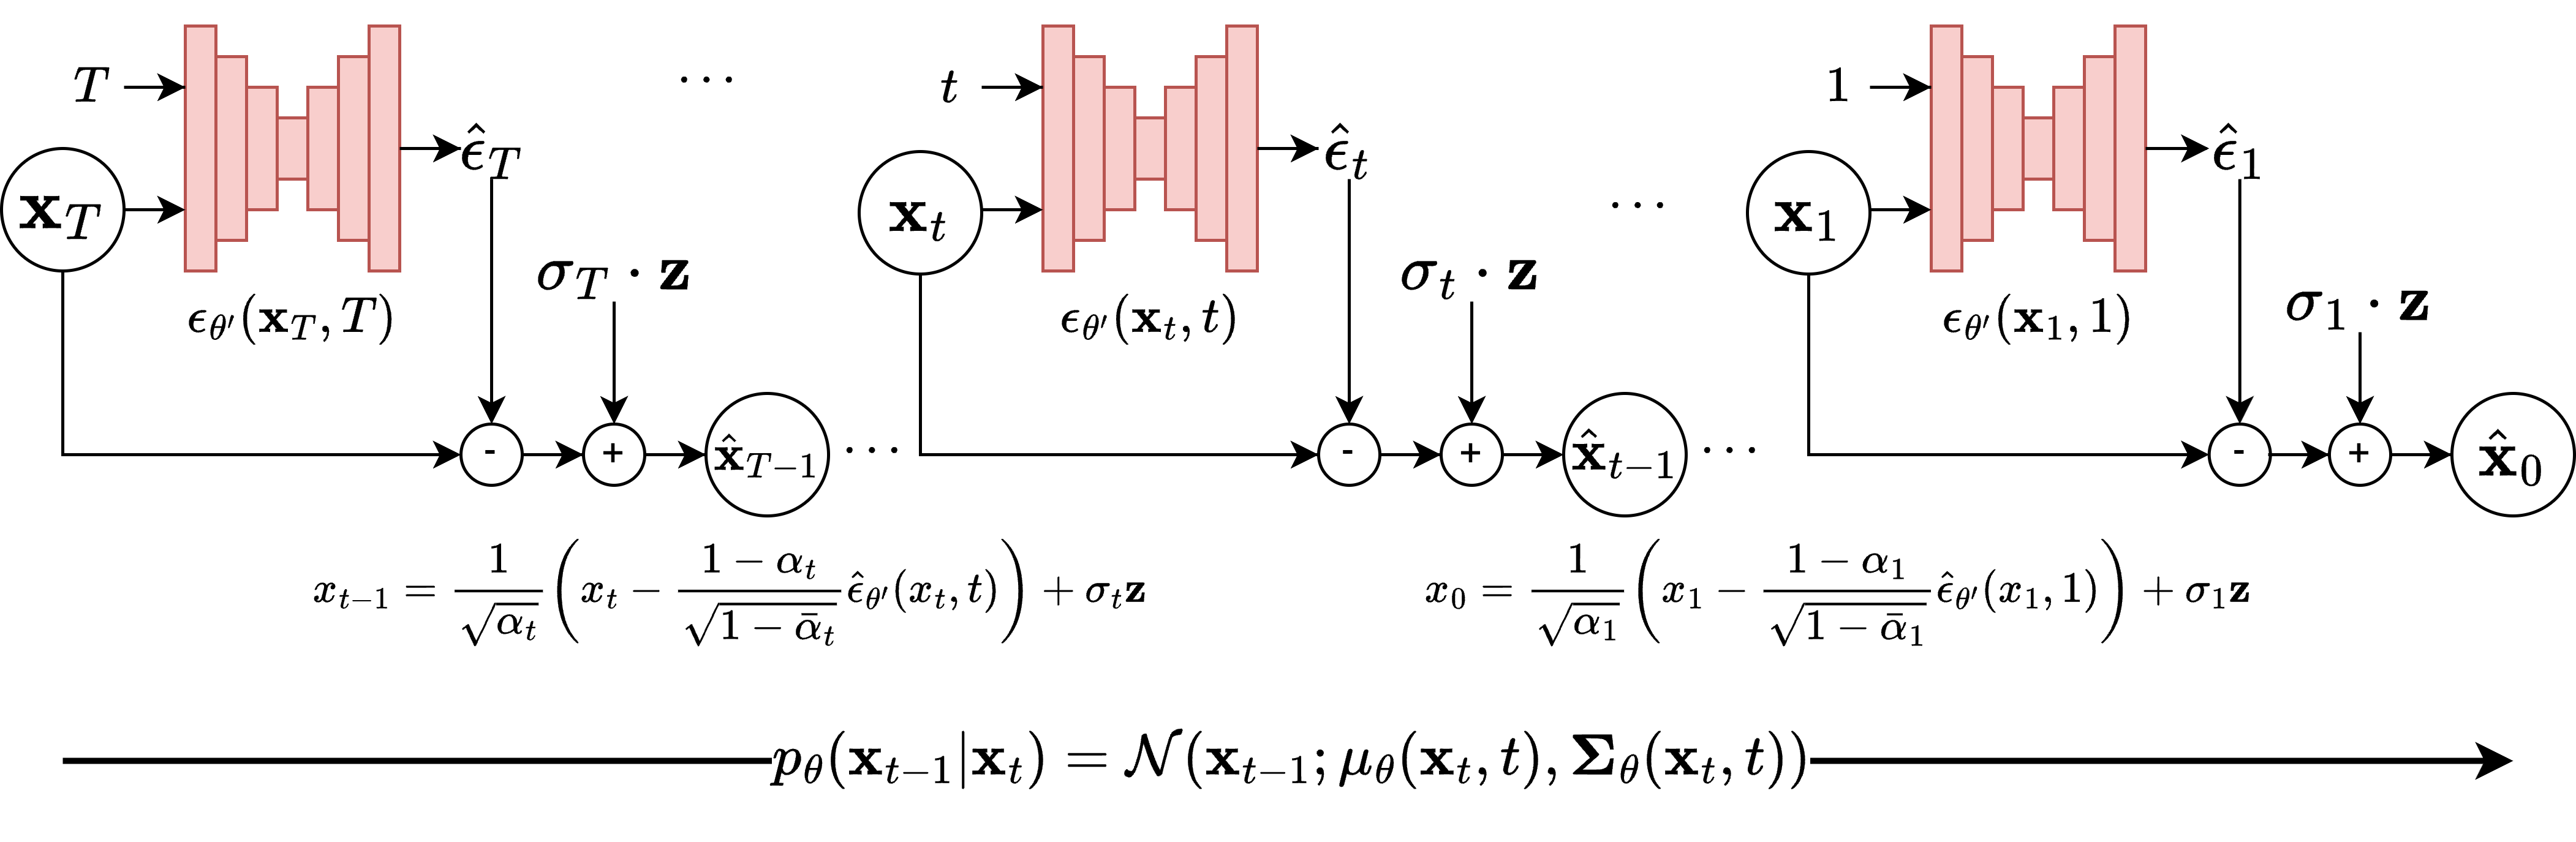
\includegraphics[width=\linewidth]{DDPMSampling}
	\end{figure}
\end{frame}

\begin{frame}{Các bước lấy mẫu với DDPM}
	
	\begin{enumerate}
		\item Bắt đầu với nhiễu: $\bx_T \sim \mathcal{N}(0, \mathbf{I})$
		\item Các giá trị $\sqrt{\alpha_t}$ $\sqrt{1 - \alpha_t}$ và $\sqrt{\bar{\alpha}_t}$ có được từ bước huấn luyện
		\item Tính hệ số điều chỉnh nhiễu $\sigma_t$ từ $\alpha_t$ ở mọi bước $t: 1 \rightarrow T$
		$\sigma_t = \sqrt{\frac{1 - \bar{\alpha}_{t-1}}{1 - \bar{\alpha}_t} (1 - \alpha_t)}$
		
		\item $\text{for all}$ $t$, lấy $t$ \textbf{tuần tự} $t \sim [T, \dots 1]$
		\item Random nhiễu $\bz \sim \mathcal{N}(0, \mathbf{I})$
		\item Đưa $\bx_t$ vào để suy luận nhiễu $\bepsilon_{\theta'} = \bepsilon_{\theta'}(\bx_t, t)$
		\item Dùng nhiễu dự đoán để trừ đi $\bx_t$ ở bước $t$
			$$\mu =  \frac{1}{\sqrt{\alpha_t}}\left( \bx_t - \frac{1-\alpha_t}{\sqrt{1-\bar\alpha_t}} \bepsilon_{\theta'}(\bx_t, t) \right)$$
%			\hat{\bx}_{t-1} =
		\item Cộng thêm một lượng nhiễu $\hat{\bx}_{t-1} = \mu + \sigma_t \bz$
		\item Khi $t=1$ ta thu được $\hat{\bx}_0$ từ quá trình khử nhiễu
	\end{enumerate}
\end{frame}

%	Ta gọi $\epsilon = \mathcal{N}(0, I)$
%\begin{columns}
%\begin{column}{0.8\textwidth}
%\begin{figure}
%	\centering
%	\includegraphics[width=\textwidth]{OverviewDiffusion}
%\end{figure}
%\end{column}
%
%\begin{column}{0.2\textwidth}
%
%\end{column}
%\end{columns}
%\\
%q(\mathbf{x}_t \vert \mathbf{x}_{t-1}) &= \mathcal{N}(\mathbf{x}_t; \sqrt{\alpha_t} \mathbf{x}_{t-1}, (1 - \alpha_t)\mathbf{I}) \\ 
%\rightarrow q(\mathbf{x}_t \vert \mathbf{x}_0) &= \mathcal{N}(\mathbf{x}_t; \sqrt{\bar{\alpha}_t} \mathbf{x}_0, (1 - \bar{\alpha}_t)\mathbf{I})

\begin{frame}{Cải tiến của  với $\mathbf{x}_0$ Objective (DALLE-2)}
	Những điểm cải tiến của $\mathbf{x}_0$ so với $\epsilon$ objective
	\begin{itemize}
		\item Thay vì hàm $f_{\theta}(\bx_t, t)$ dự đoán nhiễu $\epsilon_t$ thì  $f_{\theta}(\bx_t, t)$ dự đoán $\bx_0$.
		\item Sau khi có $\bx_0$ thì ta thêm nhiễu đã có từ trước (từ forward process) để được $\bx_{t-1}$
		\item Tiếp tục cho đến khi được $\hat{\bx}_0$
		
%		$$\tilde{\epsilon}\theta(x_t,t,c) = \epsilon\theta(x_t,t,\emptyset) + w[\epsilon_\theta(x_t,t,c) - \epsilon_\theta(x_t,t,\emptyset)]$$
	\end{itemize} 
	
	\begin{figure}
		\centering
		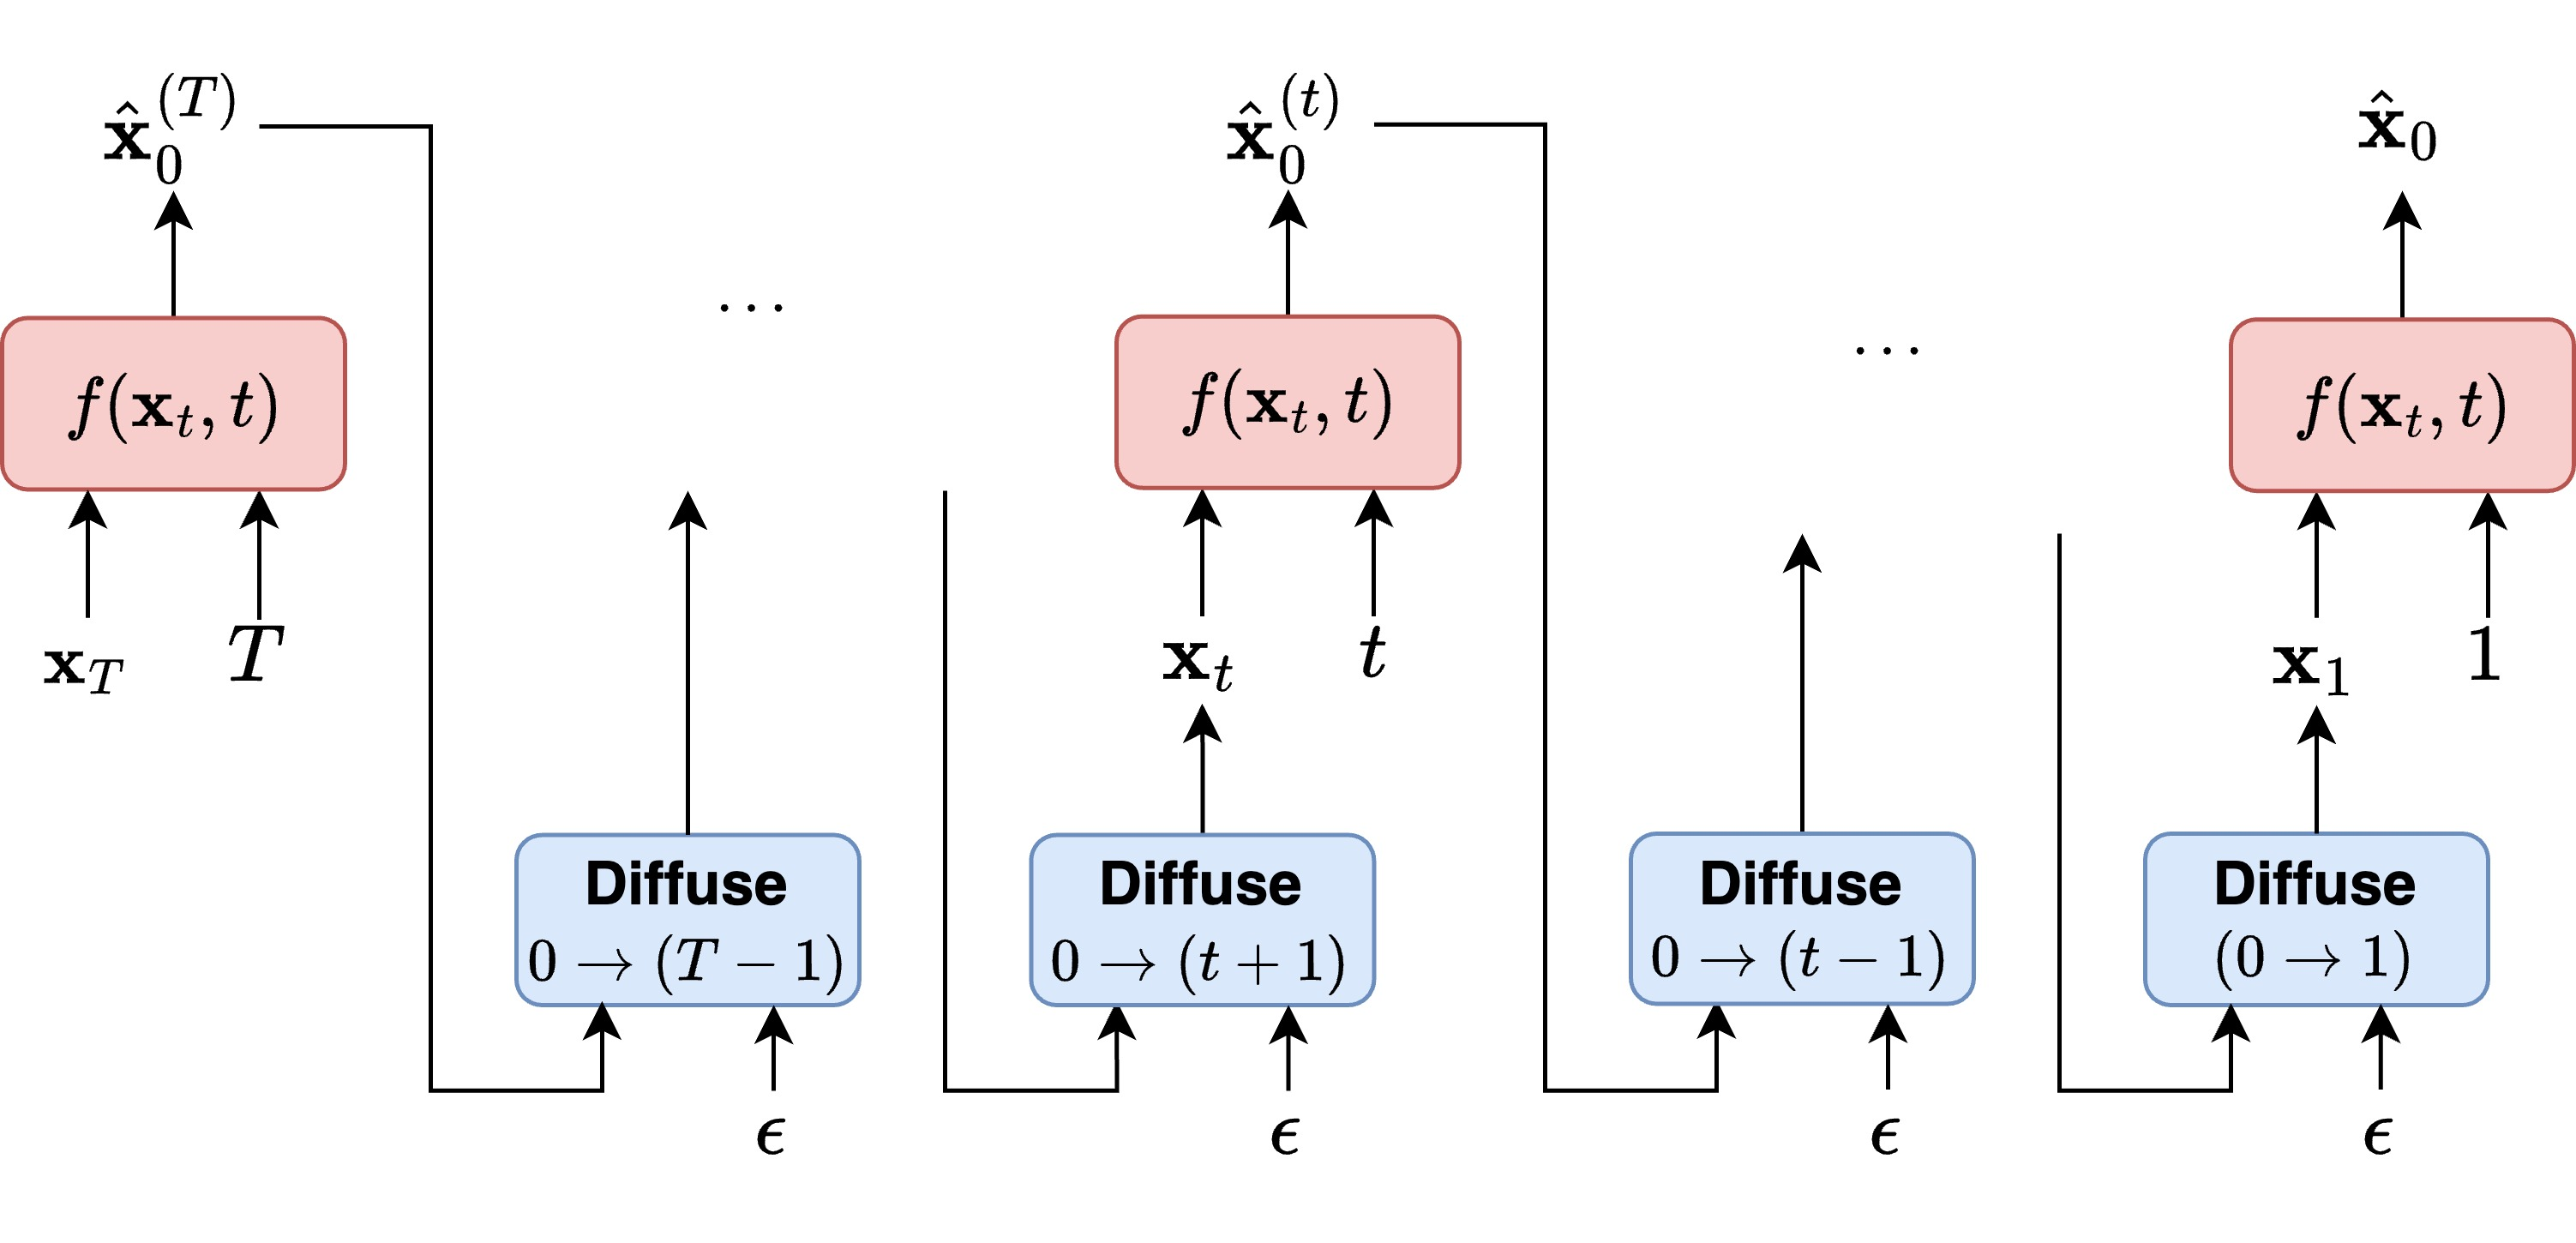
\includegraphics[width=0.95\linewidth]{SimpleX0Objective}
	\end{figure}
	
\end{frame}

\begin{frame}{So sánh $\epsilon$ objective và $\bx_0$ objective}
%$z_t = \sqrt{\bar{\alpha}_t}z_0 + \sqrt{1-\bar{\alpha}_t}\epsilon, \quad \epsilon \sim \mathcal{N}(0,I)$
%
%
%%$x_{t-1} = \sqrt{\alpha_{t-1}}\hat{x}_0 + \sqrt{1-\alpha_{t-1}}\epsilon$
%
%$\hat{z}_0 = f_\theta(z_T, t, \text{text\_embedding})$
%
%$L = \mathbb{E}_{t,z_0,\epsilon}[\|\hat{z}_0 - z_0\|_2^2]$
%
%$z_{t-1} = \sqrt{\alpha_{t-1}}\hat{z}_0 + \sqrt{1-\alpha_{t-1}}\epsilon$

\begin{figure}
	\centering
	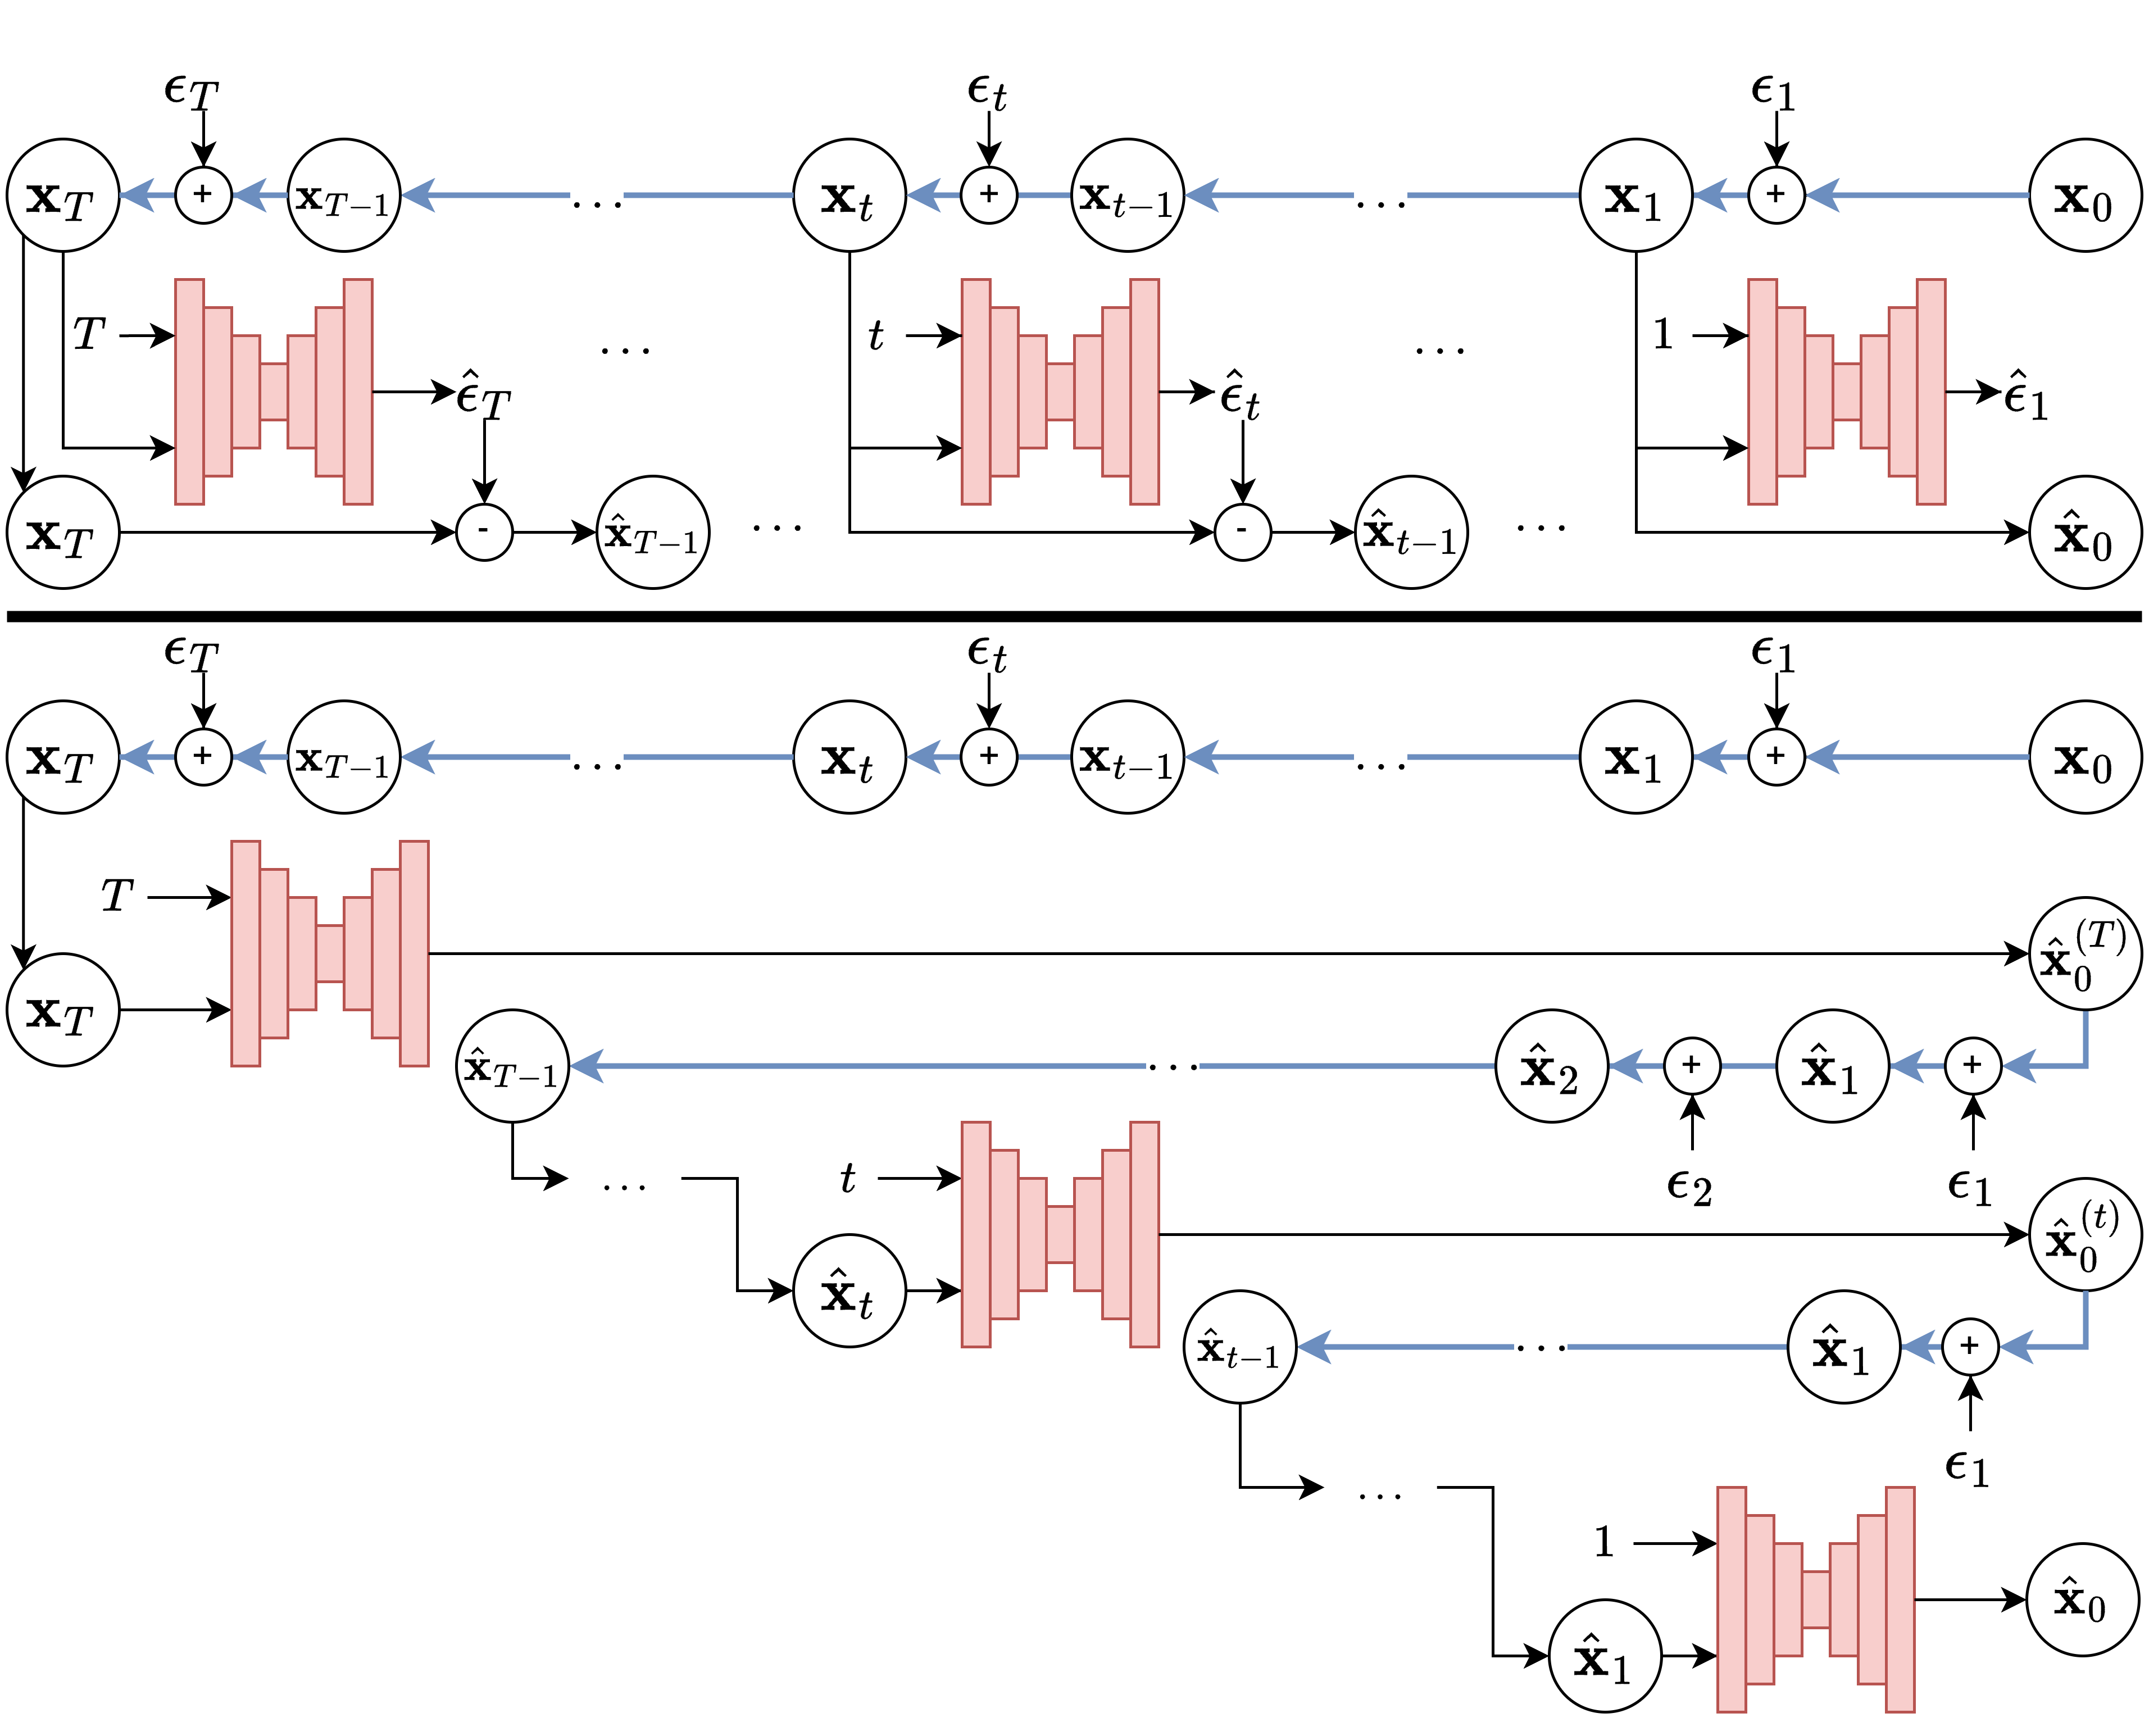
\includegraphics[width=0.95\linewidth]{X0Objective}
\end{figure}




%	
%	{Forward Process}
%	
%	\textbf{DDPM:}
%	\begin{equation}
%		q(x_t|x_{t-1}) = \mathcal{N}(x_t; \sqrt{1-\beta_t}x_{t-1}, \beta_tI)
%	\end{equation}
%	Trong đó:
%	\begin{itemize}
%		\item $\beta_t$ là lịch nhiễu (noise schedule)
%		\item $x_t$ là ảnh ở bước $t$
%		\item $\mathcal{N}$ là phân phối chuẩn (Gaussian)
%	\end{itemize}
%	
%	\textbf{DDIM:}
%	\begin{equation}
%		q(x_t|x_0) = \mathcal{N}(x_t; \sqrt{\bar{\alpha}_t}x_0, (1-\bar{\alpha}_t)I)
%	\end{equation}
%	Trong đó:
%	\begin{itemize}
%		\item $\bar{\alpha}_t = \prod_{i=1}^t(1-\beta_i)$
%		\item $x_0$ là ảnh gốc
%	\end{itemize}
%$x_t = \sqrt{\alpha_t}x_{t-1} + \sqrt{1-\alpha_t}\epsilon$

%\text{Trong đó:}
%\begin{align*}
%	& x_t: \text{là trạng thái tại thời điểm } t \\
%	& x_{t-1}: \text{là trạng thái tại thời điểm } t-1 \\
%	& \alpha_t: \text{là tham số variance scheduling } (0 < \alpha_t < 1) \\
%	& \epsilon \sim \mathcal{N}(0,1): \text{là nhiễu Gaussian}
%\end{align*}
%
%% Có thể viết dưới dạng tích lũy \bar{\alpha}
%$\text{Định nghĩa: } \bar{\alpha_t} = \prod_{i=1}^t \alpha_i$
%
%$x_t = \sqrt{\bar{\alpha_t}}x_0 + \sqrt{1-\bar{\alpha_t}}\epsilon$

%	$$\bx_{t-1} = \sqrt{\alpha_{t-1}} \left( \frac{\bx_t - \sqrt{\alpha_t} \epsilon_{\theta}(\bx_t, t)}{\sqrt{1 - \alpha_t}} \right) + \sqrt{1 - \alpha_{t-1}} \epsilon_{\theta}(\bx_t, t)$$
\end{frame}

\begin{frame}{Classifier-Free Guidance}
	\begin{columns}
		\begin{column}{0.5\textwidth}
			Để có thể học được có điều kiện (condition $c$):
%			\begin{align*}
%				\nabla p_{\gamma}(\bx_t | y) &= \nabla \log p(x_t) + \gamma \nabla p(y | \bx_t)
%			\end{align*}
%			
%			\begin{align*}
%				\nabla_{\mathbf{x}_t} \log q(\mathbf{x}_t, y)
%				&= \nabla_{\mathbf{x}_t} \log q(\mathbf{x}_t) + \nabla_{\mathbf{x}_t} \log q(y \vert \mathbf{x}_t)		
%			\end{align*}
			
		\end{column}
		
		\begin{column}{0.5\textwidth}
			\begin{figure}
				\centering
				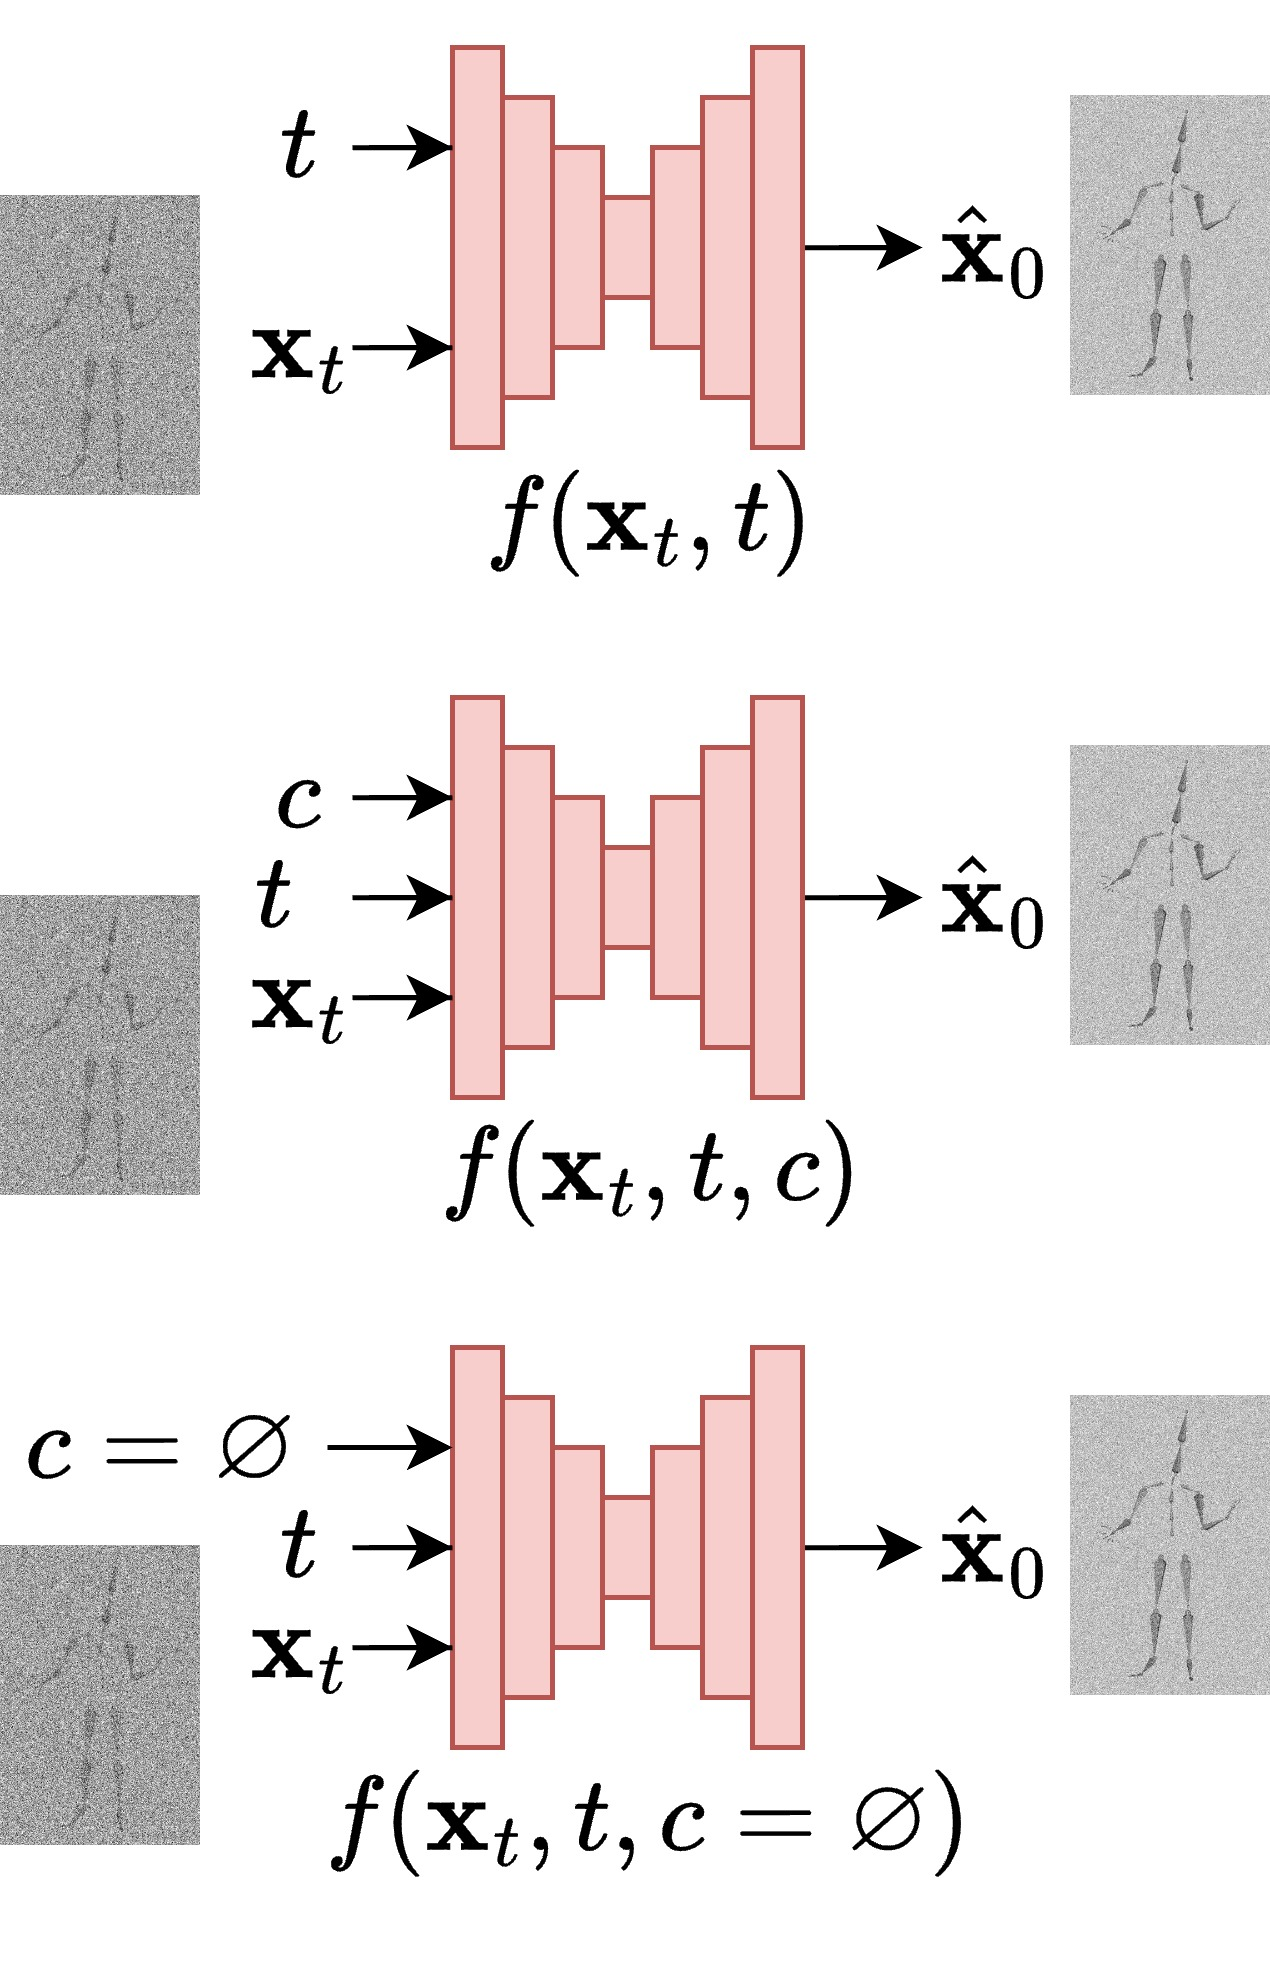
\includegraphics[width=0.95\linewidth]{ConditionDiffusion}
			\end{figure}
		\end{column}
	\end{columns}
	

	
\end{frame}


\begin{frame}{Condition Diffusion với $\mathbf{x}_0$ Objective}
	\begin{figure}
		\centering
		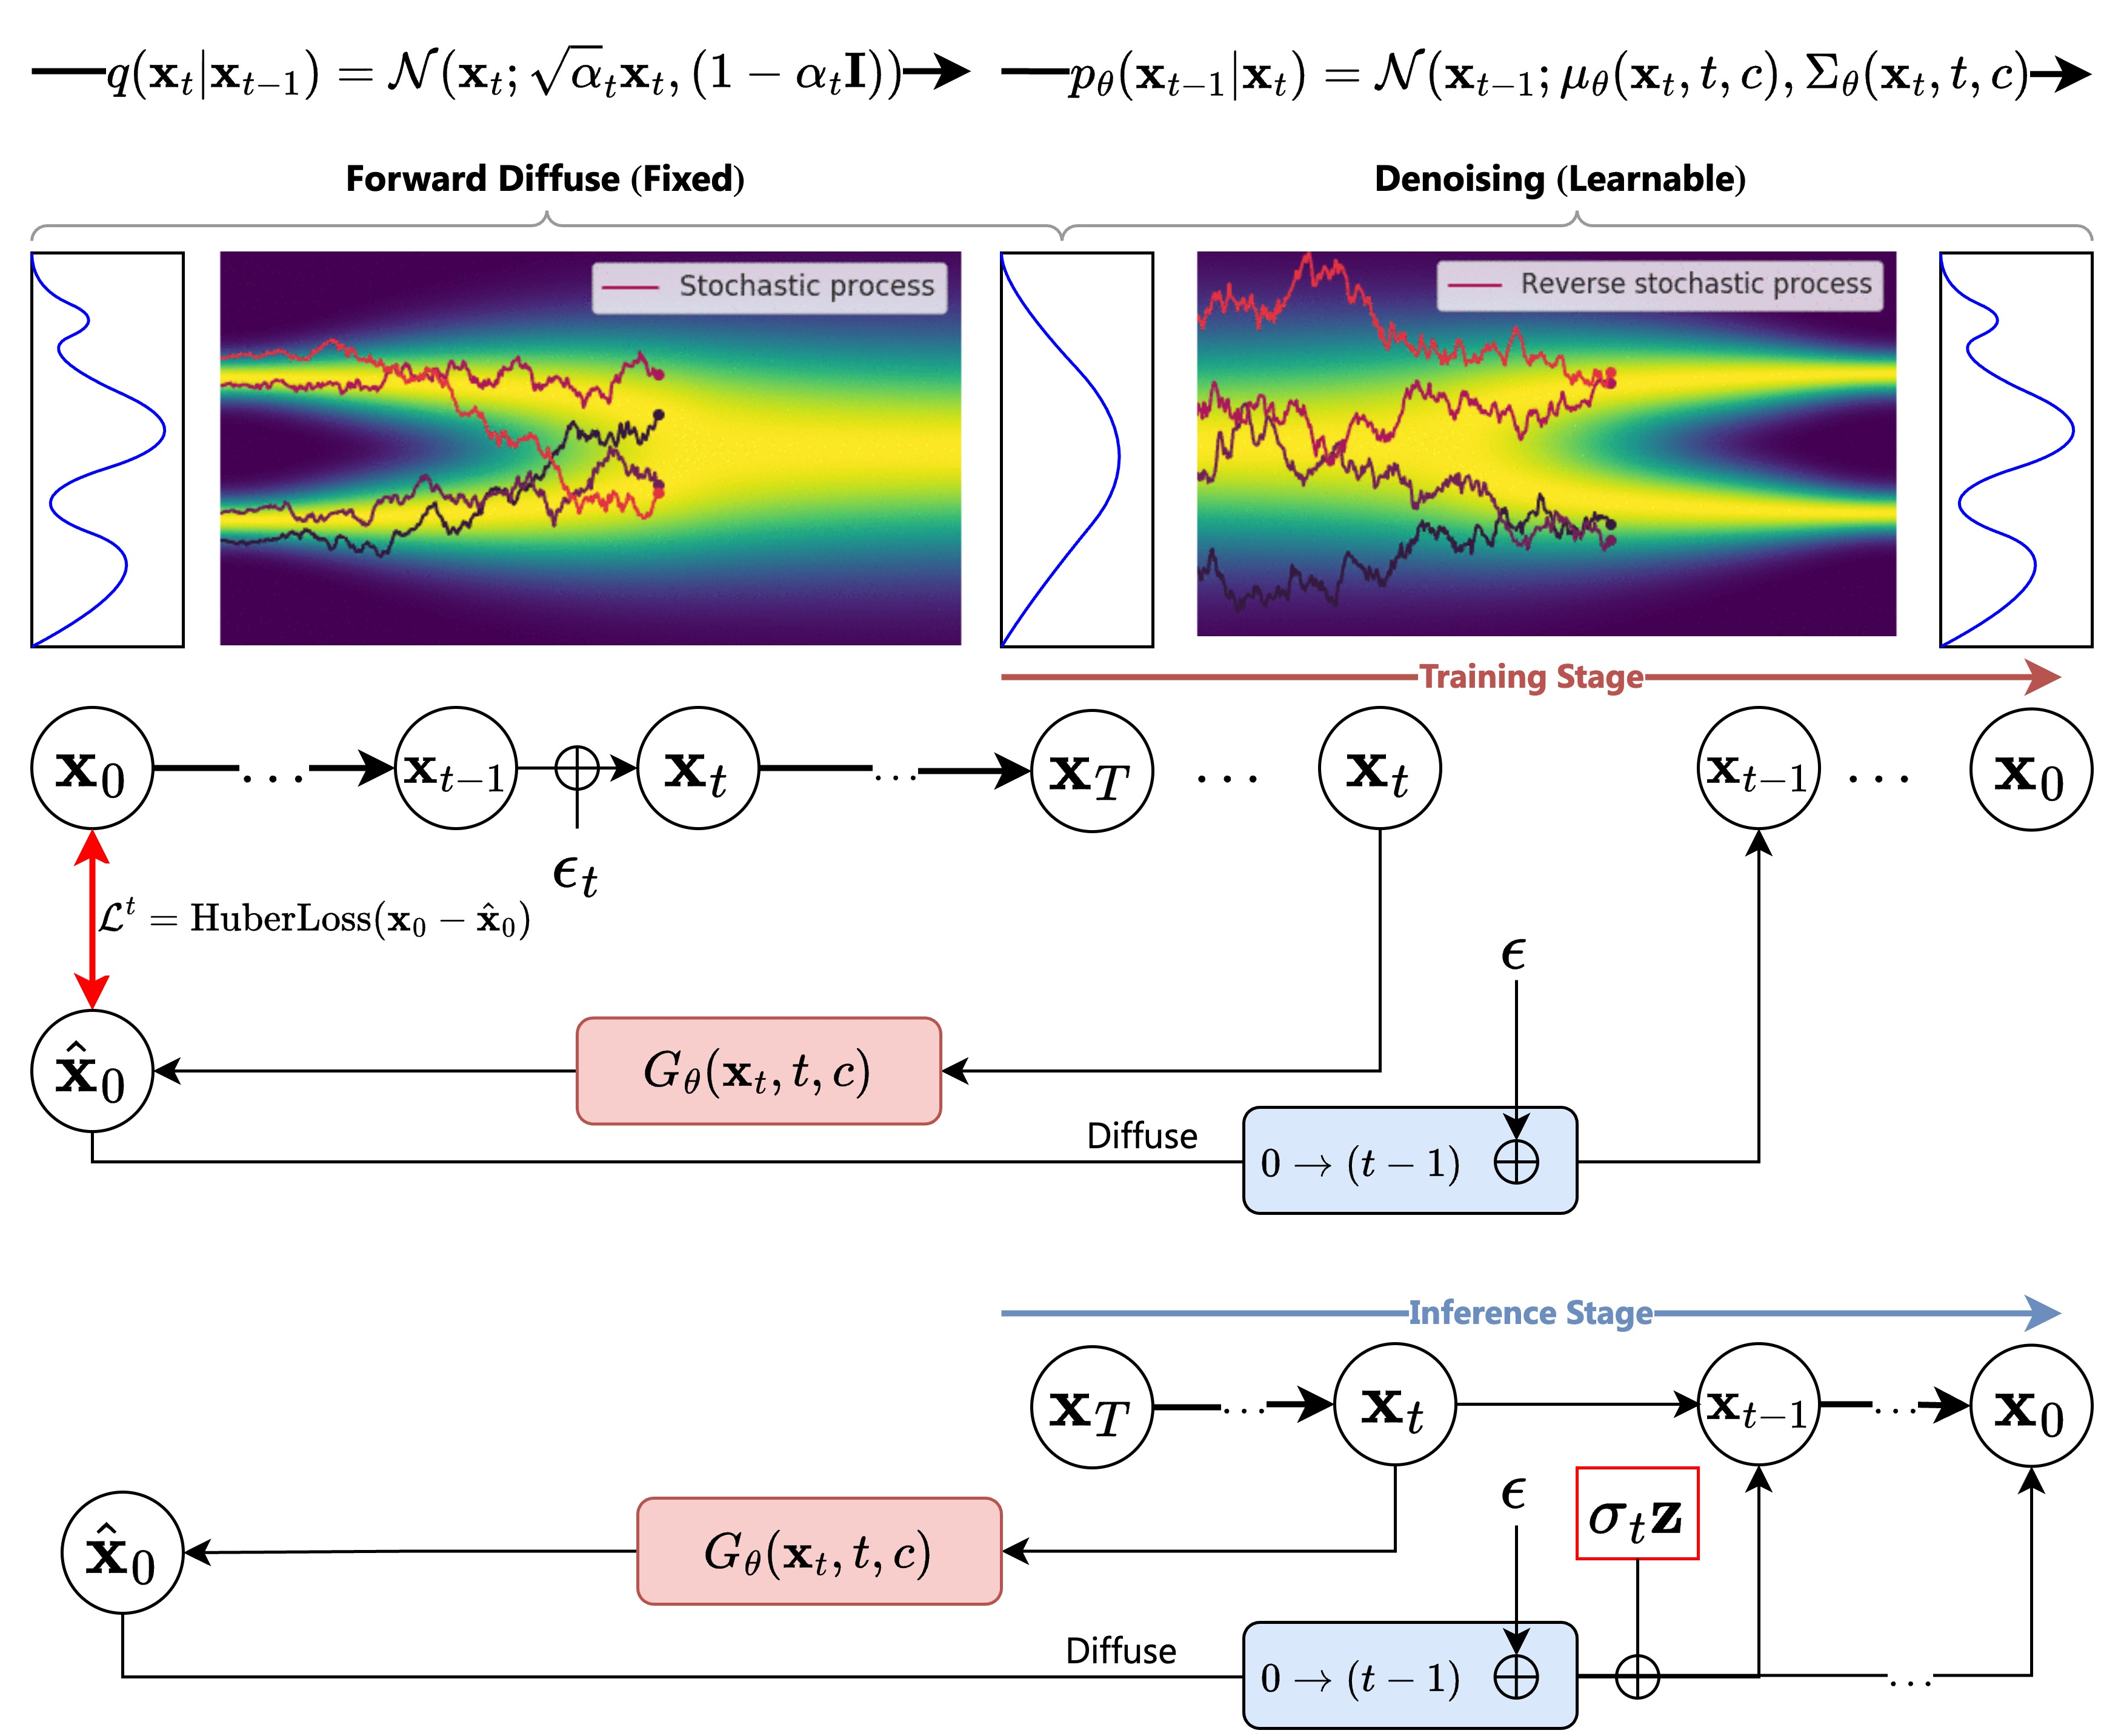
\includegraphics[width=0.95\linewidth]{TrainingAndSampling.jpg}
	\end{figure}
\end{frame}




\begin{frame}{Forward Diffusion Process}
%	 & \text{ ;where } \boldsymbol{\epsilon}_{t-1}, \boldsymbol{\epsilon}_{t-2}, \dots \sim \mathcal{N}(\mathbf{0}, \mathbf{I})
\small
\begin{itemize}[]
	\item Đặt $\alpha_t = 1 - \beta_t$, $\bar{\alpha}_t = \prod_{i=1}^t \alpha_i$
\end{itemize}
\vspace{-15pt}
\begin{align*}
	\mathbf{x}_t & = \sqrt{\alpha_t}\mathbf{x}_{t-1} + \sqrt{1 - \alpha_t} \boldsymbol{\epsilon}_{t-1} \\
						& = \sqrt{\alpha_t \alpha_{t-1}} \mathbf{x}_{t-2} + \sqrt{1 - \alpha_t \alpha_{t-1}} \bar{\boldsymbol{\epsilon}}_{t-2} \\
						& = \dots \\
						& = \sqrt{\bar{\alpha}_t}\mathbf{x}_0 + \sqrt{1 - \bar{\alpha}_t}\boldsymbol{\epsilon} \\
						q(\mathbf{x}_t \vert \mathbf{x}_{t-1}) &= \mathcal{N}(\mathbf{x}_t; \sqrt{\alpha_t} \mathbf{x}_{t-1}, (1 - \alpha_t)\mathbf{I}) \\ 
						\rightarrow q(\mathbf{x}_t \vert \mathbf{x}_0) &= \mathcal{N}(\mathbf{x}_t; \sqrt{\bar{\alpha}_t} \mathbf{x}_0, (1 - \bar{\alpha}_t)\mathbf{I})
\end{align*}
\vspace{-20pt}
%\begin{figure*}
	
%	& \text{ ;where } \bar{\boldsymbol{\epsilon}}_{t-2} \text{ merges two Gaussians (*).} \\
\begin{columns}
\begin{column}{0.5\textwidth}
	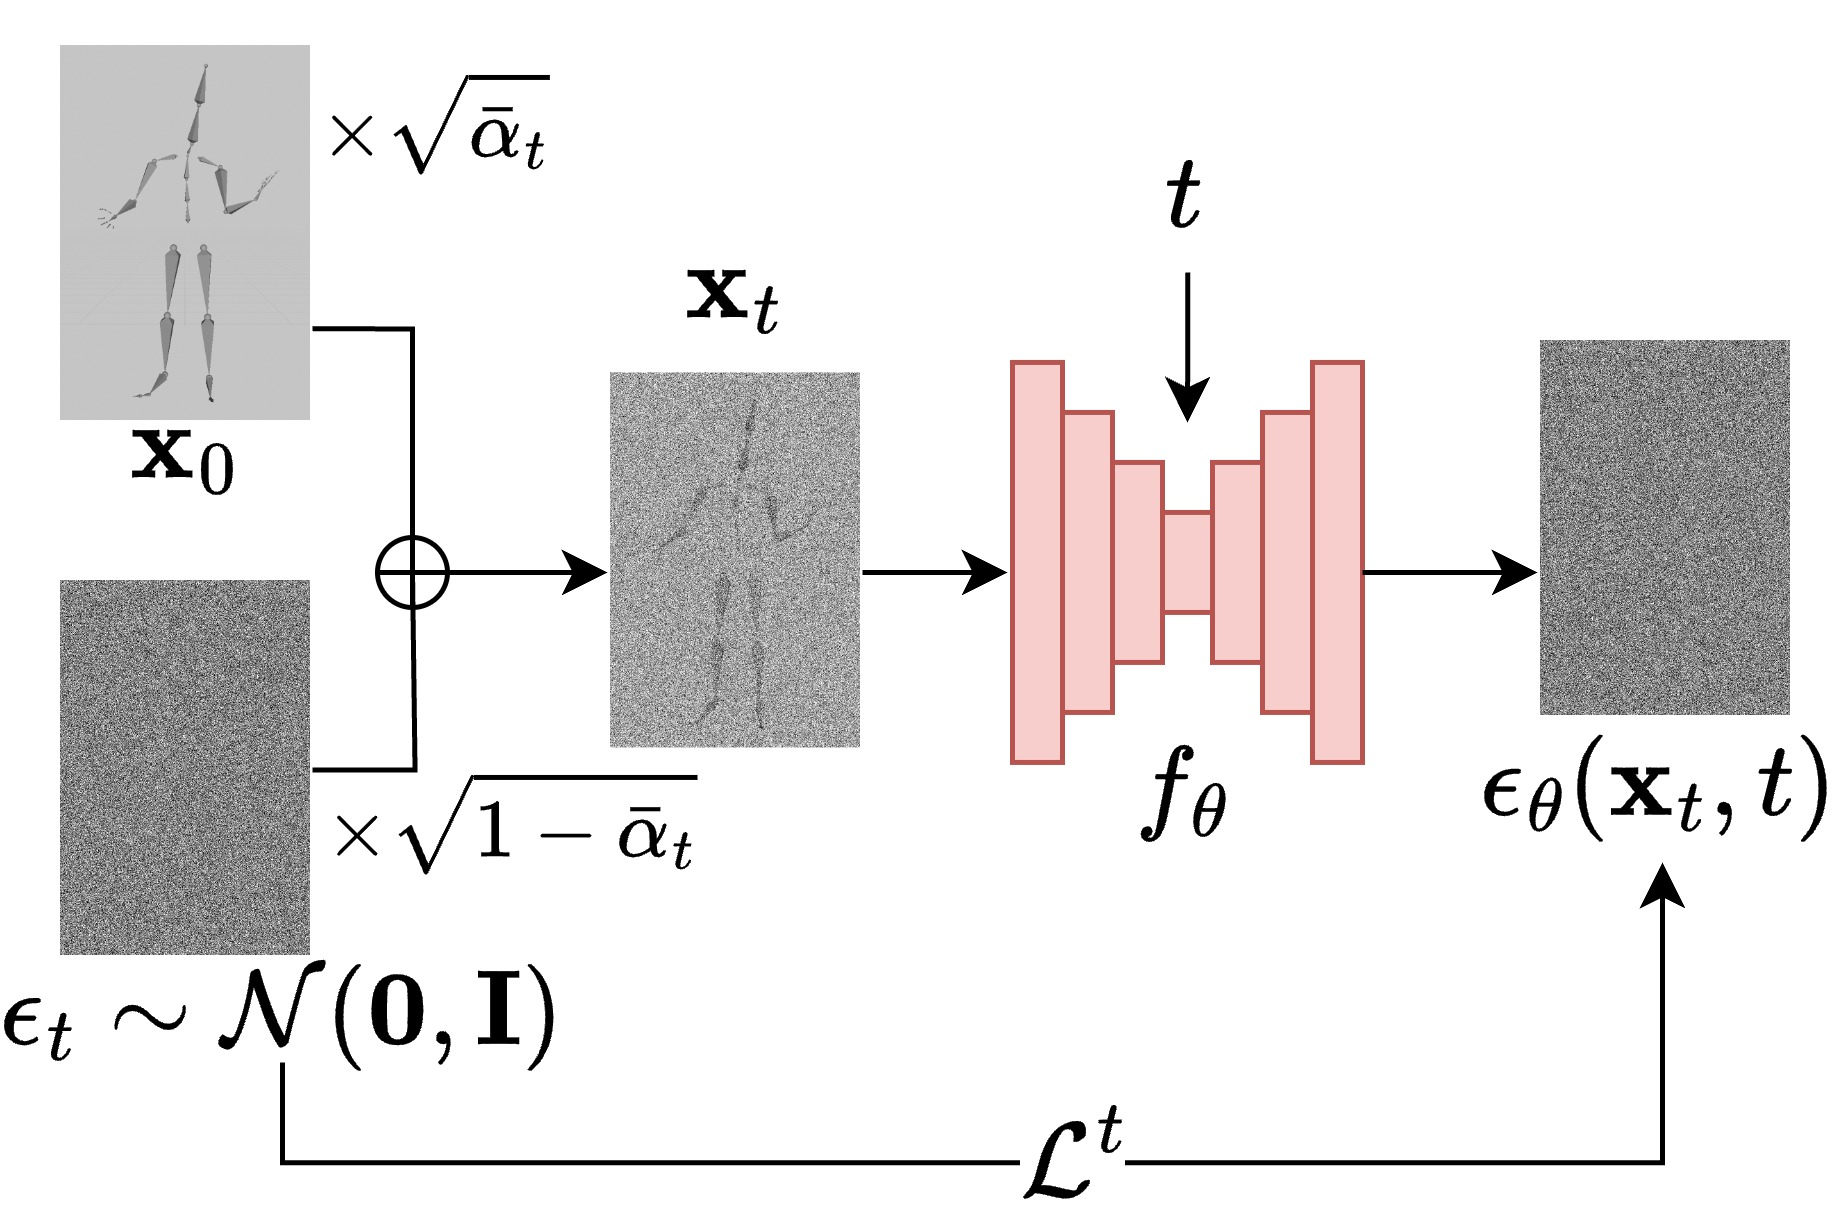
\includegraphics[width=\textwidth]{AlgorithmForwardDiffusion.png}
\end{column}


	
\begin{column}{0.5\textwidth}
	\footnotesize
	\begin{algorithm}[H]
		\caption{Training} \label{alg:training}
		\begin{algorithmic}[1]
			\footnotesize
			\Repeat
			\State $\bx_0 \sim q(\bx_0)$
			\State $t \sim \mathrm{Uniform}(\{1, \dotsc, T\})$
			\State $\bepsilon\sim\mathcal{N}(\bzero,\bI)$
			\State Take gradient descent step on
			\Statex $\qquad \grad_\theta \left\| \bepsilon - \bepsilon_\theta(\mathbf{x}_t, t) \right\|^2$
			\Until{converged}
		\end{algorithmic}
	\end{algorithm}
\end{column}
\end{columns}
\end{frame}

\begin{frame}{Reverse Diffusion Process}
	
\small
$p_{\theta}(\mathbf{x}_T) = \mathcal{N} (0, \mathbf{I}) \qquad 
p_{\theta}(\mathbf{x}_{t-1} | \mathbf{x}_t) = \mathcal{N}(\mathbf{x}_t; \mu_\theta(\mathbf{x}_t), \sigma_t^2 \mathbf{z})
$
%\begin{columns}
%	\begin{column}{0.5\textwidth}
%		
%	\end{column}
%	\begin{column}{0.5\textwidth}
%		
%	\end{column}
%\end{columns}

$\mu_\theta(\mathbf{x}_t) = 
\frac{1}{\sqrt{\alpha_{t}}} ( \mathbf{x}_t - 
\frac{1-\alpha_t}{ \sqrt{1 - \bar{\alpha_{t}} }}
\epsilon_{\theta} (\mathbf{x}_t,t))$
%\vspace{-20pt}
%\begin{figure*}

%	& \text{ ;where } \bar{\boldsymbol{\epsilon}}_{t-2} \text{ merges two Gaussians (*).} 

\begin{columns}
	\begin{column}{0.43\textwidth}
		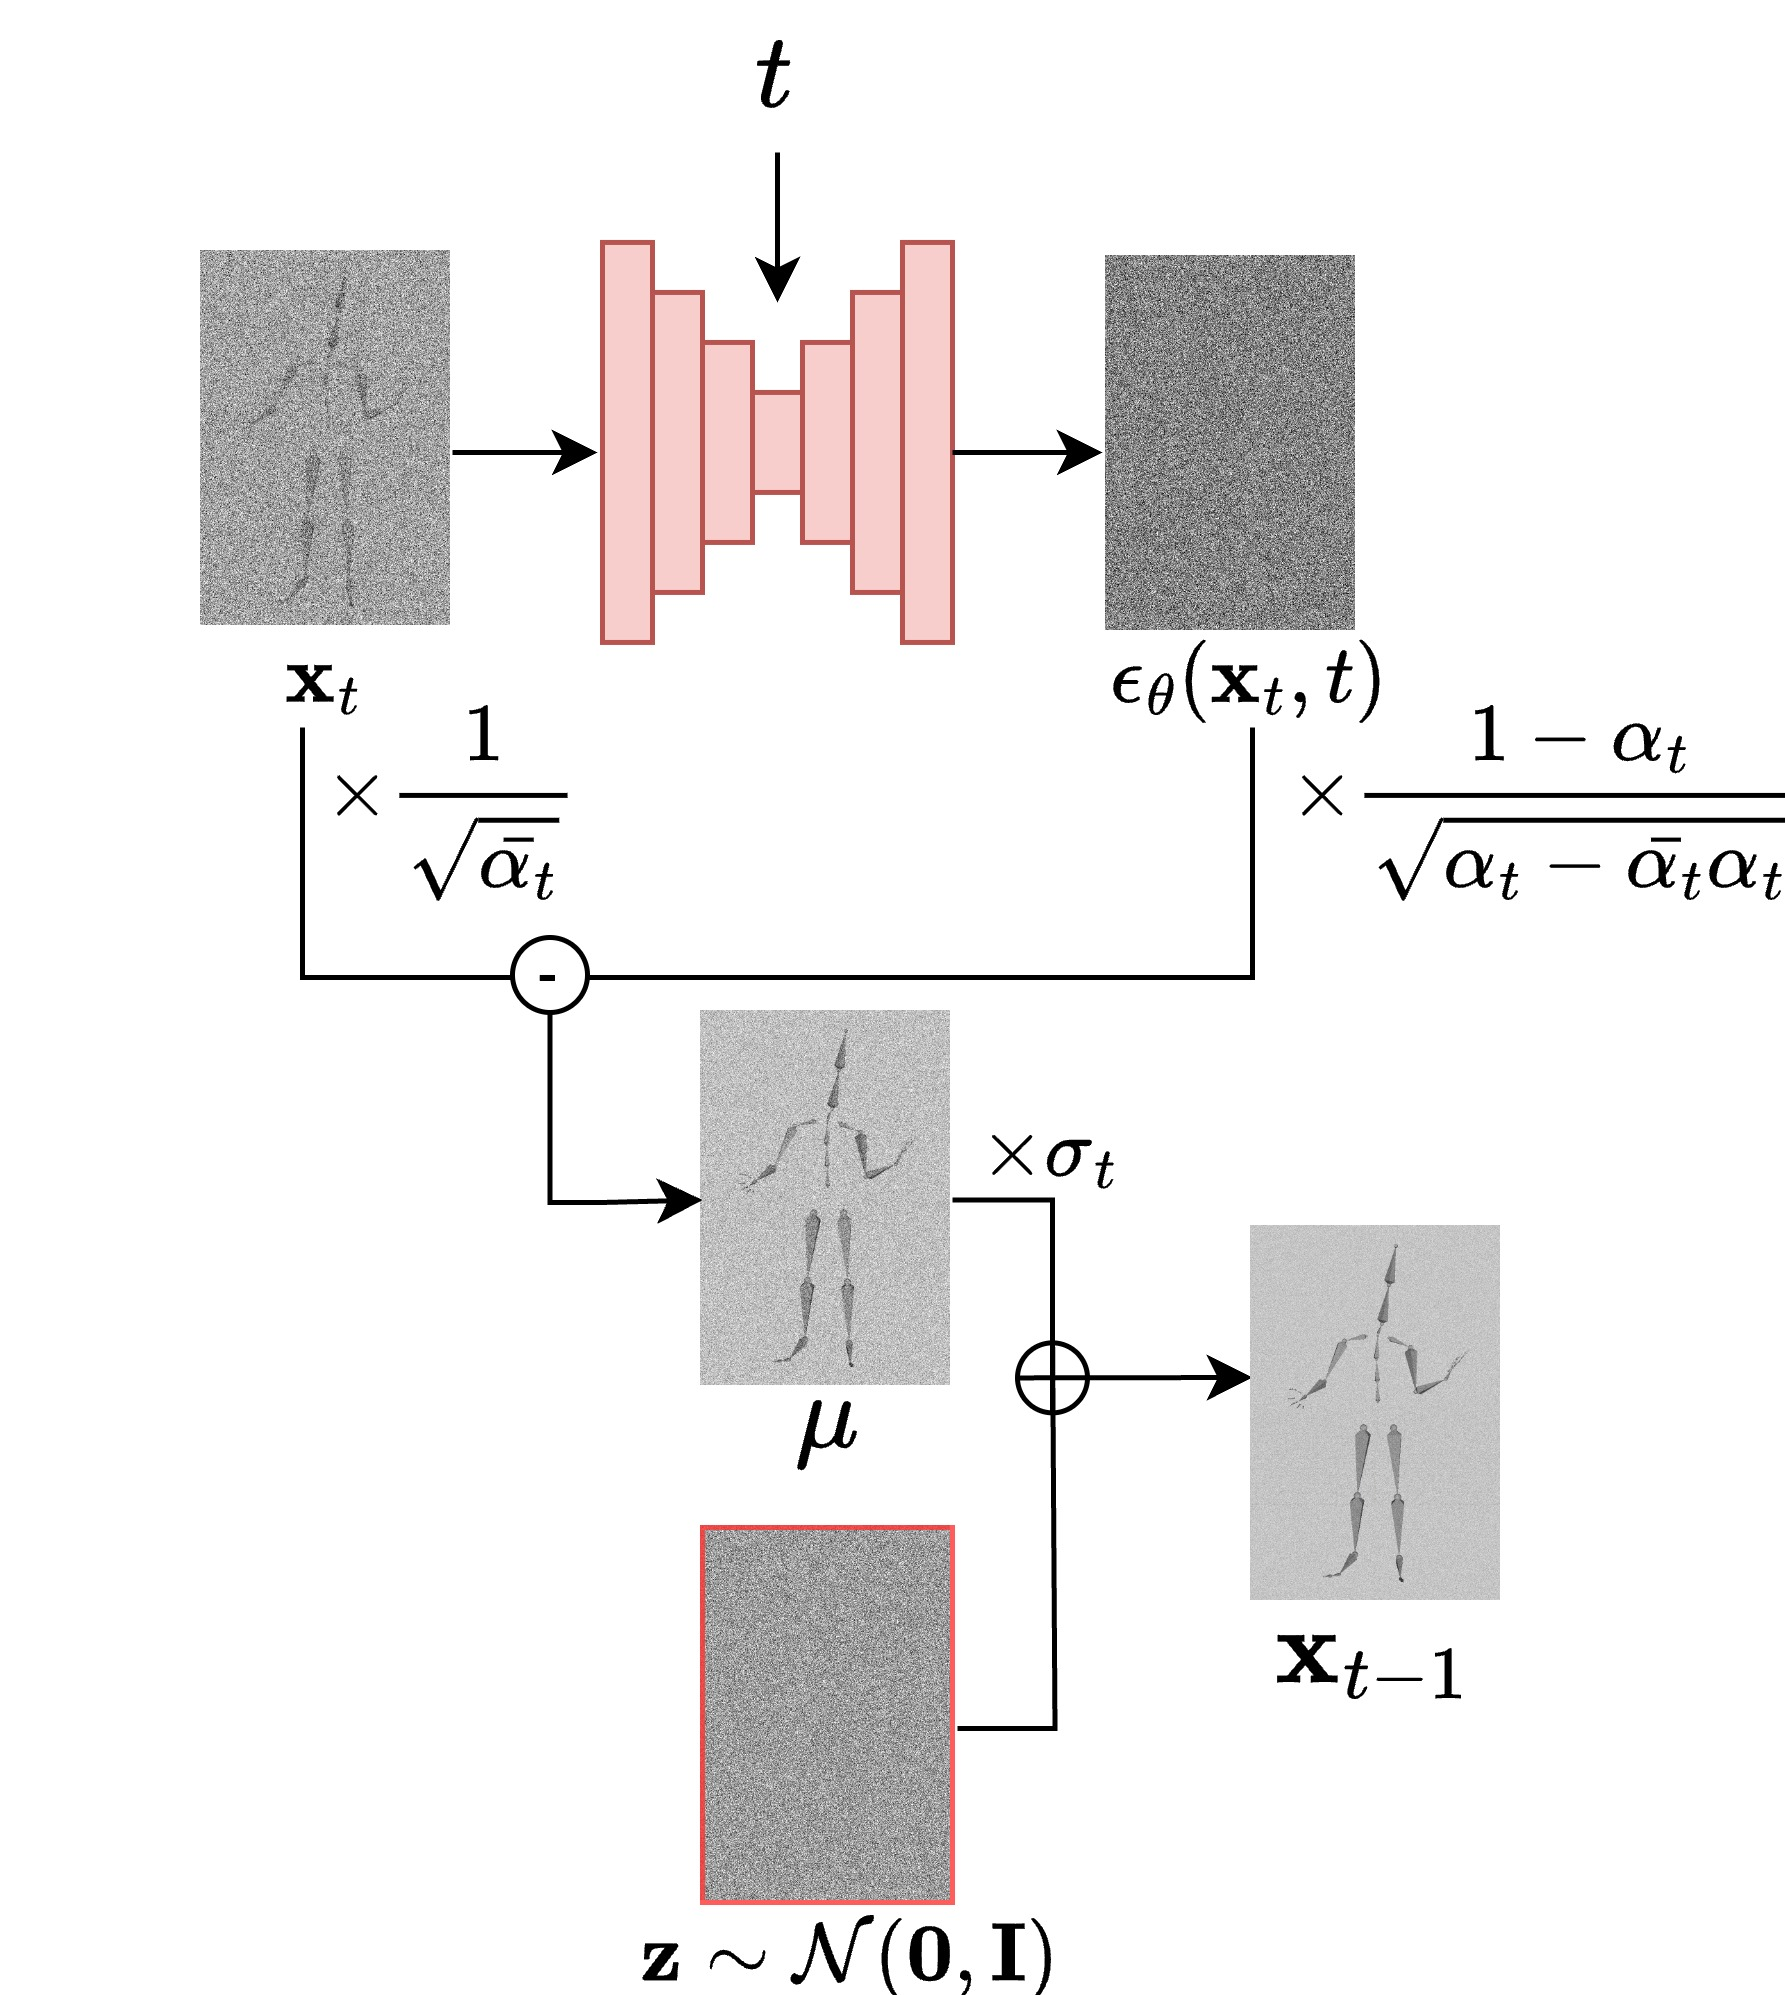
\includegraphics[width=\textwidth]{AlgorithmSamplingDiffusion.png}
	\end{column}
	
	\begin{column}{0.57\textwidth}
		\footnotesize
		\begin{algorithm}[H]
			\caption{Sampling} \label{alg:sampling}
			\footnotesize
			\begin{algorithmic}[1]
					\footnotesize
					\State $\bx_T \sim \mathcal{N}(\bzero, \bI)$
					\For{$t=T, \dotsc, 1$}
					\State $\bz \sim \mathcal{N}(\bzero, \bI)$ if $t > 1$, else $\bz = \bzero$
					\State $\mu = \frac{1}{\sqrt{\alpha_t}}\left( \bx_t - \frac{1-\alpha_t}{\sqrt{1-\bar\alpha_t}} \bepsilon_\theta(\bx_t, t) \right) $
					\State $\bx_{t-1} = \mu + \sigma_t \bz$
%					+ \sigma_t \bz
%_\theta (\mathbf{x}_t,	 t)
					\EndFor
					\State \textbf{return} $\bx_0$
					\vspace{.04in}
				\end{algorithmic}
		\end{algorithm}
\end{column}

\end{columns}

\end{frame}

%	\algrenewcommand\algorithmicindent{0.5em}
%	\begin{figure}[t]
	%		\begin{minipage}[t]{0.495\textwidth}
		%			\begin{algorithm}[H]
			%				\caption{Training} \label{alg:training}
			%				\small
			%				\begin{algorithmic}[1]
				%					\Repeat
				%					\State $\bx_0 \sim q(\bx_0)$
				%					\State $t \sim \mathrm{Uniform}(\{1, \dotsc, T\})$
				%					\State $\bepsilon\sim\mathcal{N}(\bzero,\bI)$
				%					\State Take gradient descent step on
				%				\Statex $\qquad \grad_\theta \left\| \bepsilon - \bepsilon_\theta(\sqrt{\bar\alpha_t} \bx_0 + \sqrt{1-\bar\alpha_t}\bepsilon, t) \right\|^2$
				%					\Until{converged}
				%				\end{algorithmic}
			%			\end{algorithm}
		%		\end{minipage}
	%		\begin{minipage}[t]{0.495\textwidth}
		%			
		%		\end{minipage}
	%		\vspace{-1em}
	%	\end{figure}




	
%	
%		if $L$ is not known (usually the case), can use the following line search:
%	\noindent\rule[-5pt]{\textwidth}{0.4pt}
%	
%	\noindent\rule[10pt]{\textwidth}{0.4pt}
%	
%	typical value of $\beta$ is $1/2$, and 
%	\[
%	\hat{f}_\lambda(x,y) = f(y) + \nabla f(y)^T (x - y) + 
%	(1/2\lambda)\|x - y\|_2^2
%	\]


\section{Mô hình sinh cử chỉ}

\begin{frame}{Diffusion cho bài toán sinh cử chỉ}
	\textbf{Điểm giống}
	\begin{itemize}
		\item Diffusion \cite{yang2023diffusestylegesture} trên cử chỉ $\bx^{1:M \times D}$ (như width và height trong ảnh).
		\begin{itemize}
			\item $M$ : frame theo thời gian
			\item $D=1141$ : đặc trưng khung xương của từng khung hình
		\end{itemize}
		\item Classifier-Free Diffusion với $\bx_0$ objective. Latent vector $256$.
		\end{itemize}
		
		\textbf{Điểm khác}
		
		\begin{itemize}
			\item Sinh có điều kiện:
			\begin{itemize}
				\item Điều kiện cảm xúc: $c = \big[ \mathbf{s}, \mathbf{e}, \mathbf{a}, \mathbf{v} \big]$ và $c_{\varnothing} = \big[ \varnothing, \varnothing, \mathbf{a}, \mathbf{v}\big]$.
				\item Nội suy trạng thái giữa hai cảm xúc $\mathbf{e}_1, \mathbf{e}_2$: $c = \big[ \mathbf{s}, \mathbf{e}_1, \mathbf{a}, \mathbf{v} \big]$ và $c_{\varnothing} = \big[ \mathbf{s}, \mathbf{e}_2, \mathbf{a}, \mathbf{v} \big]$.
			\end{itemize}
			\item Self-Attention: Mối liên hệ giữa các cảm xúc, cử chỉ khởi tạo và từng frame (tương tự DALL-E 2 - mối liên hệ giữa văn bản và ảnh).
			\item Concat âm thanh và văn bản (Giống ControlNet)
%			\item Học mối liên hệ giữa điều kiện và các frame bằng Local-Cross Attention
		\end{itemize}
\end{frame}



\begin{frame}{Công đoạn 2: Xử lý đặc trưng}
	%	Sử dụng mô hình Diffusion Classifier-Free Guidance (có điều kiện) với cử chỉ $\bx^{1:M \times D}$ làm $\bx_0$ và điều kiện $c = [{\mathbf{s}, \mathbf{a}, \mathbf{e}}, \mathbf{v}]$. $N = 8$, $M = 80 \sim \text{4 giây}$
	%	\vspace{-15pt}
	%	$N=8$ khung hình đầu làm khởi tạo và $M=80$ khung hình để dự đoán
	
	\begin{figure}
		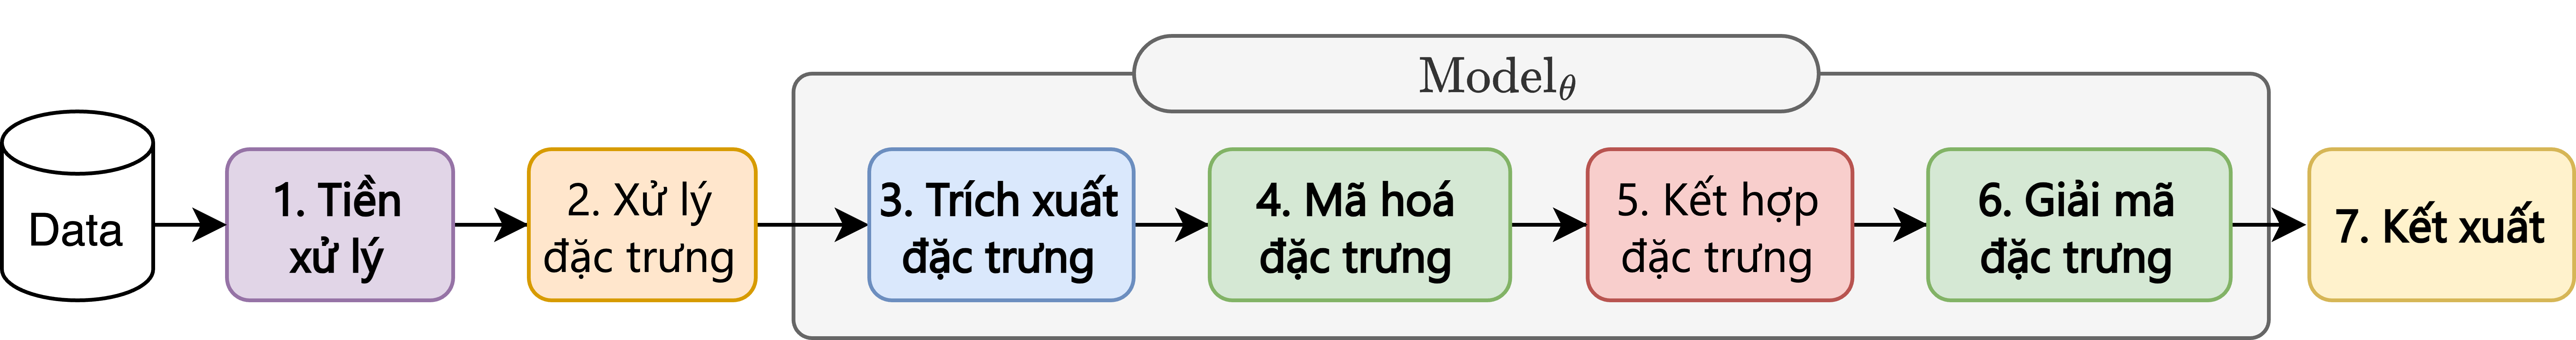
\includegraphics[width=\textwidth]{TotalStage}
	\end{figure}
	%\textbf{Âm thanh}
	
	%Cử chỉ được chuẩn hoá $\mu( \mathbf{g}) = 0$ và $\sigma = 1$. $\bx_{i} = \frac{\bx_{i} - \mu}{\sigma}$.
	\begin{itemize}
		\item \textbf{Cử chỉ}: Chuẩn hoá dữ liệu. $\mathbf{g}^{\operatorname{length}} \xrightarrow{ \text{Cắt thành đoạn} }$ $\mathbf{g}^{[N + M] \times D}$
		\begin{itemize}
			\item Cử chỉ khởi tạo: $\mathbf{s} \in \mathbb{R}^{[1:N] \times D}$
			\item Cử chỉ ground truth: $\mathbf{x} \in \mathbb{R}^{[1:M] \times D}$
		\end{itemize}
%		 \pause
		
		\item \textbf{Âm thanh}:  $\mathbf{a}^{\operatorname{length}} \xrightarrow{ \text{Cắt thành đoạn} } \mathbf{a}^{64000} \xrightarrow{\text{WavLM} } $ $\mathbf{a} \in \mathbb{R}^{[1:M] \times 1024}$ 
%		\pause
		
		%	16000
		\item \textbf{Cảm xúc}:   Nhãn $\texttt{"Happy"} \rightarrow$ $\mathbf{e} \in \mathbb{R}^{6}$ 
%		\pause
		
		\item \textbf{Văn bản}:  $\mathbf{v}^{\operatorname{length}} \xrightarrow{ \text{Cắt theo TextGrid} } \mathbf{v}^{[1:M]} \xrightarrow{ \text{FastText} } $ $\mathbf{v} \in \mathbb{R}^{[1:M] \times 300}$
	\end{itemize}
	
\end{frame}

\begin{frame}{Công đoạn 3. Trích xuất các đặc trưng}
	
	\begin{figure}
		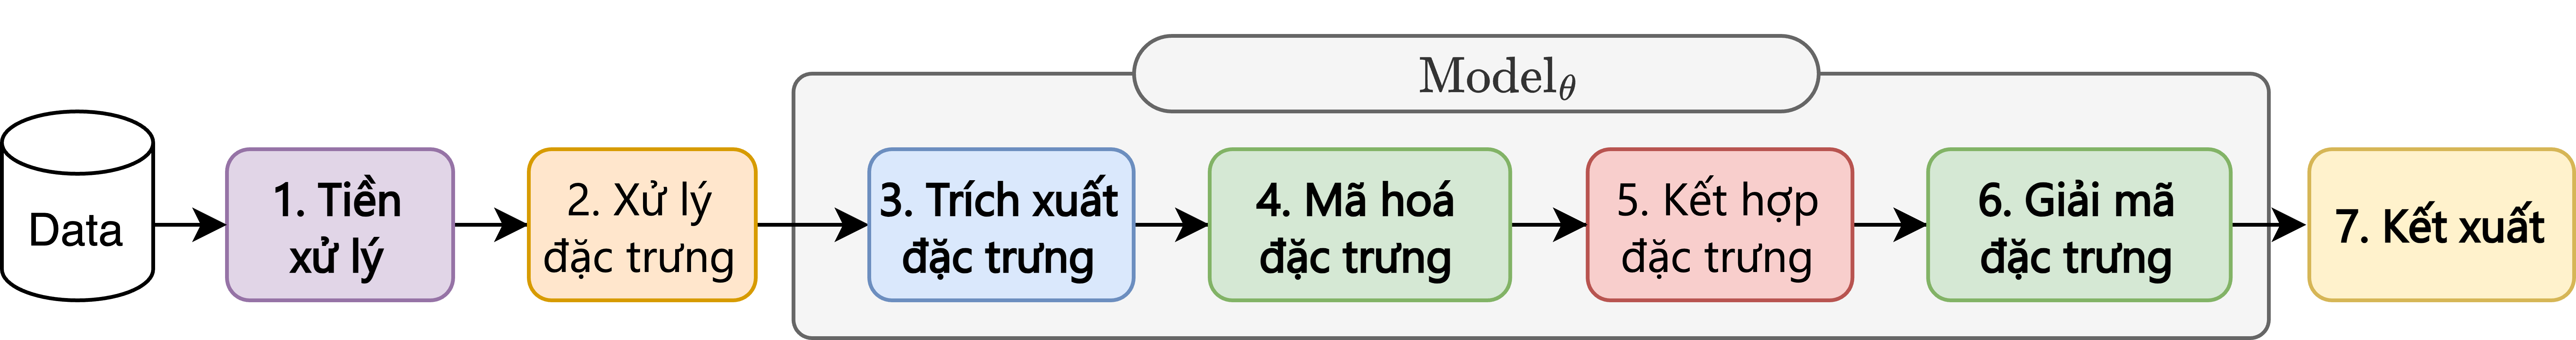
\includegraphics[width=\textwidth]{TotalStage}
	\end{figure}
	\vspace{10pt}
	\begin{itemize}
		\item Âm thanh: $\mathbf{a} \in \mathbb{R}^{ [1:M] \times 1024} \xrightarrow{\text{Linear} } \mathbf{A} \in \mathbb{R}^{[1:M] \times 64}$
		\item Cử chỉ khởi tạo: $\mathbf{s} \in \mathbb{R}^{[1:N] \times D}  \xrightarrow{\text{Linear + Random Mask} } \mathbf{S} \in \mathbb{R}^{192} $ 
		\item Cảm xúc: $\mathbf{e} \in \mathbb{R}^{6}  \xrightarrow{\text{Linear + Random Mask} } \mathbf{E} \in \mathbb{R}^{64} $ 
		\item Văn bản: $\mathbf{v} \in \mathbb{R}^{[1:M] \times 300}  \xrightarrow{\text{Linear} } \mathbf{V} \in \mathbb{R}^{256}$
		\item Timestep: $\mathbf{t} \in \mathbb{R}  \xrightarrow{\text{Linear} } \mathbf{T} \in \mathbb{R}^{256} $ 
		
		
	\end{itemize}
\end{frame}
	
%\begin{frame}{Tổng quan các công đoạn}
%	\begin{figure}
%		\centering
%		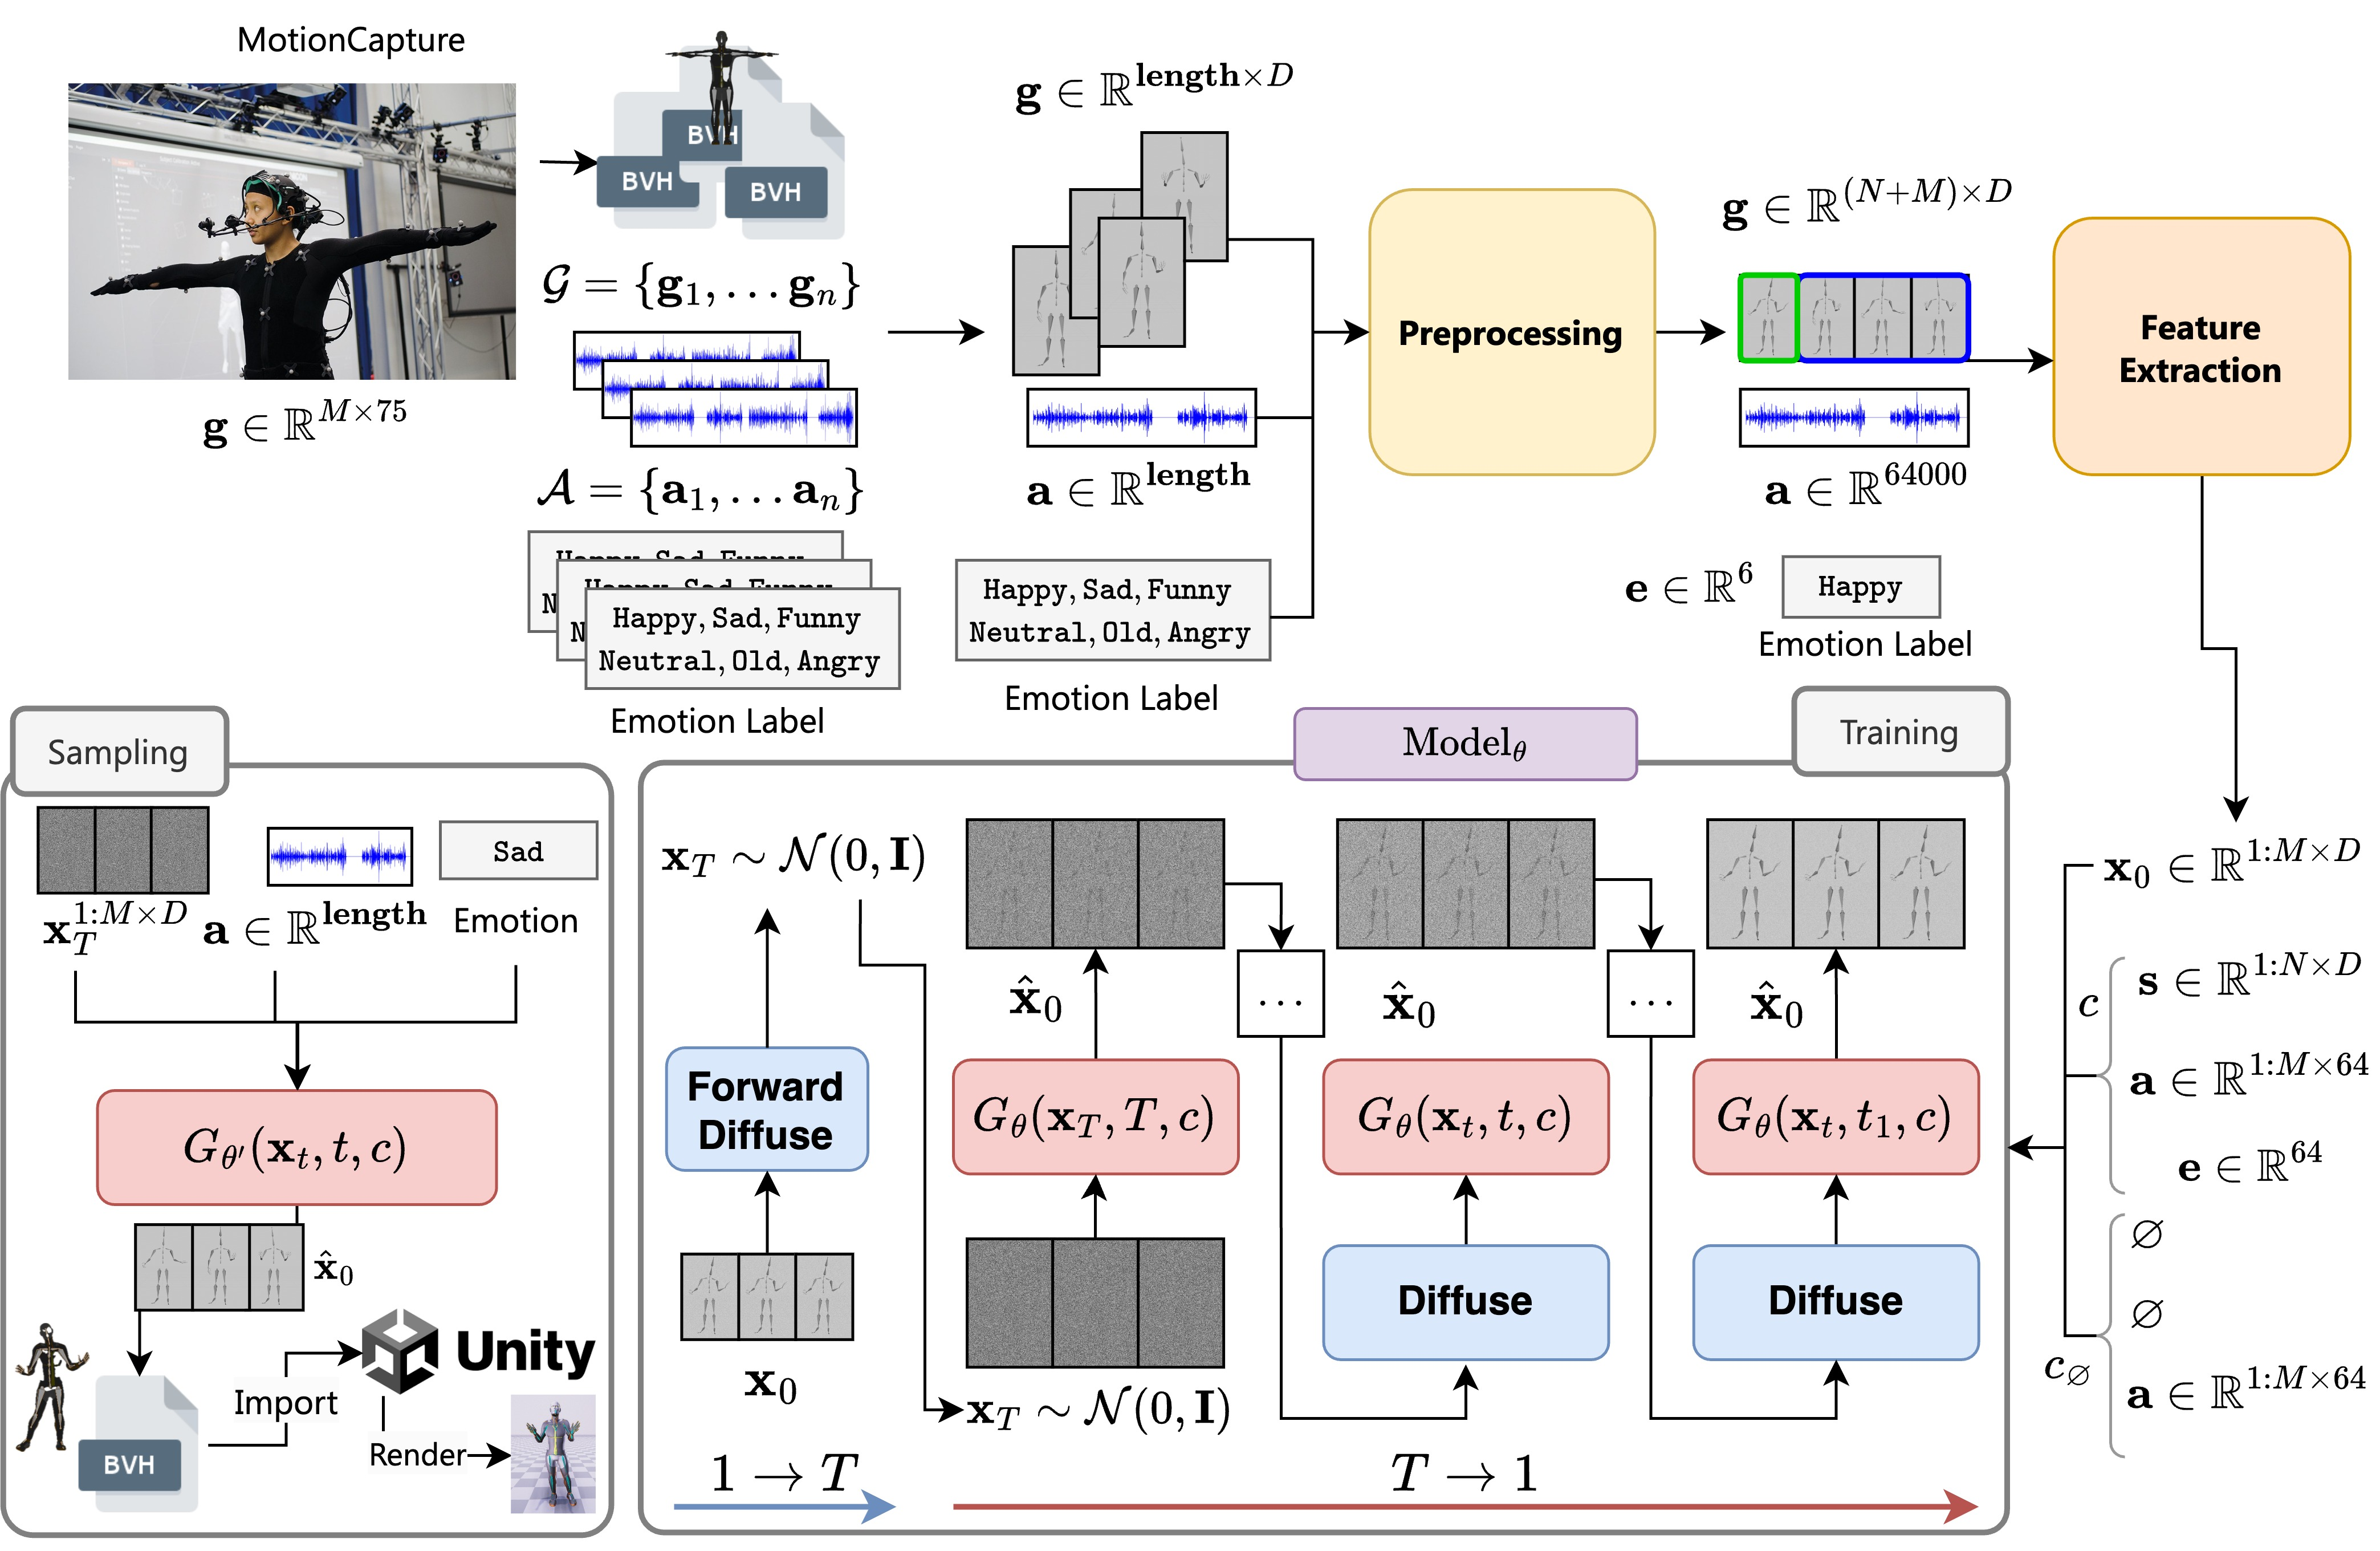
\includegraphics[width=\linewidth]{AllStage}
%	\end{figure}
%	
%\end{frame}

\begin{frame}{Công đoạn 4, 6: Mã hoá và giải mã đặc trưng}
	\begin{figure}
		\centering
		\includegraphics[width=\linewidth]{ModelStage}
	\end{figure}
\end{frame}

%\begin{frame}{Các công đoạn trong mô hình OHGesture}
%	\begin{figure}
%		\centering
%		\includegraphics[width=\linewidth]{ModelStage}
%	\end{figure}
%\end{frame}

\begin{frame}{Quá trình học Online và Offline}
	\begin{figure}
		\centering
		\includegraphics[width=\linewidth]{OnlineAndOffline}
	\end{figure}
\end{frame}


\begin{frame}{Công đoạn 5: Kết hợp các đặc trưng}
%	Cross-Local Attention and Self-Attention
%	\begin{figure}
%		\centering
%		\includegraphics[width=0.7\textwidth]{CrossLocalAttention}
%	\end{figure}
	%	\textbf{Cross-Local Attention}
	%	\begin{equation*} \label{eq:attention}
		%		\operatorname{Attention}(\mathbf{Q}, \mathbf{K}, \mathbf{V}, \mathbf{M})=\operatorname{softmax}\left(\frac{\mathbf{Q} \mathbf{K}^{T}+\mathbf{M}}{\sqrt{C}}\right) \mathbf{V}
		%	\end{equation*}
	%	
	%
	\begin{columns}
		\begin{column}{0.5\textwidth}
				\begin{itemize}
					\item Concat cảm xúc $\mathbf{E}$ và cử chỉ khởi tạo $\mathbf{S}$ để được vector latent $\mathbf{Z} \in \mathbb{R}^{256}$
					\item Cộng vector $\mathbf{Z}$ với vector timestep $\mathbf{T}$ để được vector $\mathbf{Z}$ và replicate $\mathbf{Z}$ $M$ lần để được $\mathbf{Z} \in \mathbb{R}^{[1:M] \times 256}$
					\item Concat các đặc trưng âm thanh $\mathbf{A}$, văn bản $\mathbf{V}$, cử chỉ $\mathbf{x}_{t}$ và $\mathbf{Z}$ để được vector đặc trưng theo từng frame.
					\item Thực hiện Cross-Local Attention trên vector đặc trưng từng frame để được đặc trưng $\mathbf{h}^{[1:M]}$.
					\item Sử dụng $\mathbf{Z}$ làm $\texttt{CLS}$ token cho $\mathbf{h}^{[1:M]}$ trước khi đi qua Transformer Encoder.
				\end{itemize}
				
		\end{column}
		
		\begin{column}{0.5\textwidth}
		\begin{figure}
				\centering
				\includegraphics[width=\linewidth]{CrossLocalAttention}
			\end{figure}
	\end{column}
	\end{columns}
\end{frame}

\begin{frame}{Mô hình OHGesture}
	\begin{figure}
		\centering
		\includegraphics[width=0.9\linewidth]{OHGesture}
	\end{figure}
\end{frame}






\begin{frame}{Giải thích cơ chế Attention}
	\begin{figure}
		\centering
		\includegraphics[width=0.85\linewidth]{Attention}
	\end{figure}
\end{frame}



%\begin{frame}
%	\begin{figure}
%		\centering
%		\includegraphics[width=0.8\linewidth]{DiffusionProcess}
%	\end{figure}
%\end{frame}


%\begin{figure} 
%	\centering
%	\includegraphics[width=0.8\linewidth]{DiffusionForward}
%\end{figure}


%\begin{frame}
%	
%	$
%	\label{Gaussian}
%	q\left(x_t \mid x_{t-1}\right)=\mathcal{N}\left(x_t ; \sqrt{1-\beta_t} x_{t-1}, \beta_t \mathbf{I}\right)
%	$
%	
%	$
%	\label{eq1}
%	q\left({x}_{1:T} \mid {x}_0\right)=\prod_{t=1}^T q\left({x}_t \mid {x}_{t-1}\right)
%	$
%	$
%	p_\theta\left({x}_{t-1} \mid {x}_t\right)=\mathcal{N}\left({x}_{t-1} ; {\mu}_\theta\left({x}_t, t\right), {\Sigma}_\theta\left({x}_t, t\right)\right)
%	$
%	
%	$
%	q\left({x}_t \mid {x}_0\right)=\mathcal{N}\left({x}_t ; \sqrt{\bar{\alpha}_t} {x}_0,\left(1-\bar{\alpha}_t\right) \mathbf{I}\right)
%	$
%	
%	$
%	\hat{x}_0=G\left(x_t, t, c\right)
%	$
%\end{frame}

	
%	\begin{columns}
	%		\begin{column}{0.5\textwidth}
		%			\textbf{DDPM (stochastic sampling):}
		%			\begin{itemize}
			%			\item Predict $x_0$ from $x_t$
			%			
			%			\item Convert to $\epsilon_{pred}$
			%			
			%			\item Use the formula:
			%			
			%			$$x_{t-1} = \frac{1}{\sqrt{\alpha_t}} x_t - \frac{1-\alpha_t}{\sqrt{1-\bar{\alpha}t}\sqrt{\alpha_t}} \epsilon_{\text{pred}} + \sigma_t z$$
			%			
			%			\item where $z \sim \mathcal{N}(0,I)$ is random noise
			%			\end{itemize}
		%			
		%		\end{column}
	%		
	%		\begin{column}{0.5\textwidth}
		%			\textbf{DDIM (deterministic sampling):}
		%			
		%			Predict $x_0$ from $x_t$
		%			
		%			NO additional noise term ($\sigma_t = 0$)
		%			
		%			Use the formula:
		%			
		%			$x_{t-1} = \sqrt{\bar{\alpha}{t-1}} x_0^{\text{pred}} + \sqrt{1-\bar{\alpha}_{t-1}} \epsilon_{\text{pred}}$
		%			
		%			Where:
		%			\begin{itemize}
			%			\item $\bar{\alpha}_t$ is the cumulative product of $\alpha$'s from 1 to t
			%			\item $\epsilon_{pred}$ is derived from $x_0$ prediction using:
			%			\item $\epsilon_{pred} = \frac{x_t - \sqrt{\alpha_t}x_{0_{pred}}}{\sqrt{1-\alpha_t}}$
			%			\end{itemize}
		%		\end{column}
	%	\end{columns}
	


%
\section{Thực nghiệm}

\begin{frame}{Dataset}
	
%	$x^{2} \in \mathbb{R}^{x \times y}$

\begin{columns}
	\begin{column}{0.5\textwidth}
		ZeroEGGs Dataset
		\begin{itemize}
			\item Happy,  Sad, Neutral
			\item Old, Relaxed, Angry
		\end{itemize}
		%	\includepdf[pages=-]{images/EmotionPCA.pdf}
		\includegraphics[width=\linewidth]{EmotionPCA.pdf}
	\end{column}
	
	\begin{column}{0.5\textwidth}
		\includegraphics[width=\linewidth]{ZEGGsData}
	\end{column}
\end{columns}
\end{frame}

%\begin{frame}{Training Process}
%
%\end{frame}


%

\begin{frame}{Độ đo}
	Các độ đo trong Gesture Generation:
	\begin{itemize}
		\item Human-likeness 
		\item Gesture-Speech Appropriateness
		\item Gesture-style Appropriateness
	\item {FID (Fréchet Inception Distance)}:
%	\vspace{-5mm}
	\begin{equation*}
		\operatorname{FID} = \left\| \mu_{\operatorname{real}} - \mu_{\operatorname{fake}} \right\|^2 + \operatorname{Tr} \left( \Sigma_{\operatorname{real}} + \Sigma_{\operatorname{fake}} - 2 \left( \Sigma_{\operatorname{real}} \Sigma_{\operatorname{fake}} \right)^{\frac{1}{2}} \right)
	\end{equation*}
%	\vspace{-5mm}
	 \item Mean opinion scores (MOS)
	
\end{itemize}
\end{frame}
\begin{frame}{Kết quả}
	\begin{columns}
	\begin{column}{0.33\textwidth}
		\includegraphics[width=\linewidth]{BoxHumanLikeness.pdf}
	\end{column}
	
	\begin{column}{0.33\textwidth}
		\includegraphics[width=\linewidth]{BoxSpeechAppropriateness.pdf}
	\end{column}
	
	\begin{column}{0.33\textwidth}
		\includegraphics[width=\linewidth]{BoxStyleAppropriateness.pdf}
	\end{column}
\end{columns}

%Thử nghiệm với các thành phần cấu trúc trong mô hình:	
%
%\begin{enumerate}
%\item Sử dụng đặc trưng WavLM
%\item 
%\end{enumerate}

%\begin{itemize}
%	\item (1)sdf 
%\end{itemize}

\begin{table}[!t]
%	\footnotesize
\tiny
	\centering
	\resizebox{\columnwidth}{!}{%
		\begin{tabular}{lcc}
			\hline
			\multicolumn{1}{c}{Name} &
			\begin{tabular}[c]{@{}c@{}}Human\\ likeness \end{tabular}$\uparrow$ &
			\begin{tabular}[c]{@{}c@{}}Gesture-speech\\ appropriateness\end{tabular}$\uparrow$ \\ \hline
			Ground Truth          & 4.15 $\pm$ 0.11          & 4.25 $\pm$ 0.09          \\
			Ours                  & \textbf{4.11 $\pm$ 0.08} & \textbf{4.11 $\pm$ 0.10} \\
			\quad$-$ WavLM             & 4.05 $\pm$ 0.10          & 3.91 $\pm$ 0.11          \\
			\quad$-$ Cross-local attention   & 3.76 $\pm$ 0.09          & 3.51 $\pm$ 0.15          \\
			\quad$-$ Self-attention    & 3.55 $\pm$ 0.13          & 3.08 $\pm$ 0.10          \\
			% \begin{tabular}[c]{@{}c@{}}$-$ attention (GRU based) \\ (GRU based)\end{tabular} &
			\quad$-$ Attention + GRU&
			3.10 $\pm$ 0.11 &
			2.98 $\pm$ 0.14 \\
			\quad$+$ Forward attention & 3.75 $\pm$ 0.15          & 3.23 $\pm$ 0.24          \\
			\hline
		\end{tabular}%
	}
%	\caption{Kết quả của các nghiên cứu loại bỏ (Ablation studies). "$-$" chỉ các mô-đun không được sử dụng và "$+$" chỉ các mô-đun bổ sung. Chữ in đậm chỉ ra chỉ số tốt nhất.}
	\label{Ab}
\end{table}

\end{frame}


%
\section{Kết luận}

\begin{frame}{Giải quyết các thách thức}
		\begin{itemize}
			\item Bằng việc dùng Cross-Local Attention và Self-Attention, chúng tôi giải quyết được quan hệ $1:n$ của cử chỉ và các điều kiện âm thanh, cảm xúc.
			\item Mô hình Diffusion giúp mô hình có thể học được các đặc trưng có phân bố dữ liệu thật thấp.
			\item Đảm bảo khả năng mở rộng (scalable) của hệ thống sinh cử chỉ để có thể ứng dụng trong thực tế.
		\end{itemize}
\end{frame}

\begin{frame}{Đóng góp chính}
	
	\begin{figure}
		\centering
		\includegraphics[width=0.9\linewidth]{TotalStage}
	\end{figure}
	
	\begin{itemize}
		\item Transcribe âm thanh để có được văn bản (\textit{Công đoạn tiền xử lý}, \textit{xử lý đặc trưng} và \textit{kết hợp đặc trưng}), làm dữ liệu bổ sung trong Diffusion có điều kiện.
		
		\item Mở rộng mã nguồn chương trình: \hyperlink{https://github.com/hmthanh/OHGesture}{\textbf{github.com/OHGesture}}, Mô hình pretrain: \hyperlink{https://huggingface.co/openhuman/openhuman}{\textbf{Huggingface.co/openhuman}}
		
		\item Giai đoạn Hệ thống trực quan hoá bằng Unity (\textit{Công đoạn Kết xuất}): \hyperlink{https://github.com/DeepGesture/deepgesture-unity}{\textbf{github.com/DeepGesture-Unity}}.
		
		\item Genea Leaderboard: Paper xây dựng hệ thống chuẩn hoá
		
		\item Đánh giá cử chỉ bằng FID: \hyperlink{https://github.com/GestureScore/GestureScore}{\textbf{github.com/GestureScore}}.
	\end{itemize}
\end{frame}

\begin{frame}[label=frame]{{Kết luận}}
	\begin{itemize}
		\item Mô hình \textbf{OHGesture}, có khả năng sinh cử chỉ chân thực, không chỉ trên các mẫu dữ liệu trong tập huấn luyện mà còn mở rộng được với những âm thanh không có trong dữ liệu huấn luyện.
		
		\item Sử dụng phương pháp \textbf{Classifier-free Guidance}, có thể điều khiển các điều kiện như cảm xúc, cử chỉ khởi tạo, có thể nội suy để suy luận ra giữa các cảm xúc khác nhau.
		
		\item Bài toán sinh cử chỉ còn rất mới, chúng tôi dự định sẽ dùng Fourier TT để trích xuất các đặc trưng về pha.
		
	\end{itemize}
	

%	In this slide, some important text will be
%	\alert{highlighted} because it's important.
%	Please, don't abuse it.
%	
%	\begin{block}{Remark}
%		Sample text
%	\end{block}
%	
%	\begin{alertblock}{Important theorem}
%		Sample text in red box
%	\end{alertblock}
%	
%	\begin{examples}
%		Sample text in green box. The title of the block is ``Examples".
%	\end{examples}
%	\hyperlink{appendix}{\beamerbutton{More on Appendix}}
\end{frame}

%

%\begin{frame}{Reference 2 s}
%	\cite{yang2023diffusestylegesture}
%\end{frame}


%\begin{frame}[allowframebreaks]{References}
%	{\footnotesize
%    \printbibliography}
%\end{frame}


%\appendix
%
%\section{Phụ lục}
%
%\begin{frame}{Ký hiệu}
%	\textbf{Tham số}: Đang huấn luyện {\Large$\textcolor{cyan}{\theta}$}, đã huấn luyện xong: {\Large$\textcolor{cyan}{\theta}'$}, {\Large$\textcolor{cyan}{\hat{\bx}}$}: dự đoán
%	\vspace{-5pt}
%	
%	\textbf{Phân phối chuẩn}
%	\vspace{-5pt}
%	{\Large $$\mathcal{N}(\textcolor{red}{a} \mathbf{x}, \textcolor{blue}{b^2})$$}
%	\vspace{-15pt}
%	\begin{itemize}
%		\item Một hàm $f(x) = a x + b\epsilon$ với $\epsilon \in \mathcal{N}(0, \mathbf{1})$ được ký hiệu là $f(x) \sim \mathcal{N}(a x, b^2) $
%		
%		\item Trung bình: $\mu = \textcolor{red}{a}x=\frac{1}{n} \sum_{i=1}^{n} x_i$
%		
%		\item Phương sai: $\sigma^2 = \textcolor{blue} {b^2} = \frac{1}{n} \sum_{i=1}^{n} (x_i - \mu)^2$
%		
%	\end{itemize}
%	\textbf{Xác xuất có điều kiện}
%	\vspace{-5pt}
%	{\Large $$p(\textcolor{green}{x}| \textcolor{orange}{y})$$}
%	\vspace{-15pt}
%	
%	\begin{itemize}
%		\item $p(\textcolor{green}{x}| \textcolor{orange}{y})$ là xác xuất có điều kiện.
%		\item $\textcolor{orange}{y}$: xảy ra trước (bên phải)
%		\item $\textcolor{green}{x}$: sảy ra sau y (bên trái)
%	\end{itemize}
%	
%\end{frame}

%
%\begin{frame}
%	%	Mỗi Bone được biểu diễn thành: 
%	%	$$q = w + xi + yj + zk$$
%	%	
%	%	$$i^2 = j^2 = k^2 = ijk = -1$$
%	\begin{figure}
%		\centering
%		\includegraphics[width=\textwidth]{BVH}
%	\end{figure}
%\end{frame}
%
%
%\begin{frame}{Góc quay của một khung xương}
%	\small
%	\textbf{Hierachy}: bao gồm 75 Bone $\{ \mathbf{t}_i \}^{75} $, có vị trí ban đầu  $\mathbf{t}_{i} = \{t_x, t_y, t_z\}$
%	
%	\vspace{5pt}
%	
%	\textbf{Bone} trong dữ liệu BVH bao gồm vị trí $\mathbf{position}_{\operatorname{local}}  \in \mathbb{R}^{3}$ và góc quay $\mathbf{rotation}_{\operatorname{local}} \in \mathbb{R}^{3}$.
%	%	\begin{figure}
%		%		\centering
%		%		\includegraphics[width=0.25\textwidth]{BVHFile}
%		%	\end{figure}
%	$\mathbf{rotation}_i^{\operatorname{local}} = \{ \alpha ,\beta , \gamma \}$ lần lượt là góc quay quanh các trục $Z$ ,$Y$ , và $X$, góc quay tổng hợp trong không gian Eule là $R = R_Z(\alpha) R_Y(\beta) R_X(\gamma)$:
%	\begin{equation}
%		\mathbf{position}_{\text{global}} = R \cdot \mathbf{position}_{\text{local}} + \mathbf{t}
%	\end{equation}
%	Chuyển góc quay từng Bone dạng Euler ZYX sang dạng Quaternion, mỗi Bone biểu diễn bằng $q = (q_w, q_x, q_y, q_z)$
%	%	Mỗi Bone được biểu diễn thành: 
%	%	$$q = w + xi + yj + zk$$
%	%	c
%	%	$$i^2 = j^2 = k^2 = ijk = -1$$
%	\begin{columns}
%		\begin{column}{0.5\textwidth}
%			\begin{itemize}
%				\item $c_{\alpha} = \cos\left(\frac{\alpha}{2}\right), \quad s_{\alpha} = \sin\left(\frac{\alpha}{2}\right)$
%				\item $c_{\beta} = \cos\left(\frac{\beta}{2}\right), \quad s_{\beta} = \sin\left(\frac{\beta}{2}\right)$
%				\item $c_{\gamma} = \cos\left(\frac{\gamma}{2}\right), \quad s_{\gamma} = \sin\left(\frac{\gamma}{2}\right)$
%			\end{itemize}
%		\end{column}
%		\begin{column}{0.5\textwidth}
%			\begin{itemize}
%				\item $q_w = c_{\alpha} c_{\beta} c_{\gamma} + s_{\alpha} s_{\beta} s_{\gamma}$
%				\item $q_x = c_{\alpha} c_{\beta} s_{\gamma} - s_{\alpha} s_{\beta} c_{\gamma}$
%				\item $q_y = c_{\alpha} s_{\beta} c_{\gamma} + s_{\alpha} c_{\beta} s_{\gamma}$
%				\item $q_z = s_{\alpha} c_{\beta} c_{\gamma} - c_{\alpha} s_{\beta} s_{\gamma}$
%			\end{itemize}
%		\end{column}
%	\end{columns}
%	\begin{equation}
%		\mathbf{p}_{\text{global}} = q \cdot \mathbf{p}_{\text{local}} \cdot q^{-1} + \mathbf{t}
%	\end{equation}
%	
%	$\mathbf{t}$ là vị trí gốc của bone trong không gian toàn cục.
%\end{frame}
%
%
%
%
%\begin{frame}{$q(\bx_t | \bx_{t-1})$ và $p_{\theta}(\bx_{t-1} | \bx_t ) $  trong DDPM }
%	\textbf{DDPM} (Denoising Diffusion Probabilistic Model \cite{ho2020denoisingdiffusionprobabilisticmodels})
%	\begin{figure}
%		\centering
%		\includegraphics[width=\textwidth]{PQ}
%	\end{figure}
%	
%	\begin{itemize}
%		\item $q (\mathbf{x}_{t} | \mathbf{x}_{t-1}) = \mathcal{N}(\mathbf{x}_t; \sqrt{\alpha}_t \mathbf{x}_t, (1 - \alpha_t \mathbf{I}))$
%		\item $p_\theta (\mathbf{x}_{t-1} | \mathbf{x}_{t}) = \mathcal{N}(\mathbf{x}_{t-1}; \mu_\theta{(\mathbf{x}_t, t)}, {\Sigma}_{\theta} {  (\mathbf{x}_t, t ) }$
%	\end{itemize}
%	%	$q(\mathbf{x}_t \vert \mathbf{x}_0) = \mathcal{N}(\mathbf{x}_t; \sqrt{\bar{\alpha}_t} \mathbf{x}_0, (1 - \bar{\alpha}_t)\mathbf{I})$
%	%
%	%
%	%
%	%\begin{equation}
%	%	\mathbf{x}_{t-1}=\frac{1}{\sqrt{1- \beta_t}}\left(\bx_t-\sqrt{\beta_t} \cdot \epsilon_{\color{red}{\theta}}\left(\mathbf{x}_t, t\right)\right)+\color{red}{\beta_t \cdot \sigma_t \mathbf{z}} \color{black}{}
%	%\end{equation}
%	
%\end{frame}
%
%\begin{frame}{Vanilla Diffusion với $\epsilon$ Objective}
%	\begin{figure}
%		\centering
%		\includegraphics[width=0.95\textwidth]{TrainingAndSamplingStandard}
%	\end{figure}
%\end{frame}
%
%
%
%
%\begin{frame}{Quan hệ $\bx_{0}$, $\bx_t$ và $\bx_{t - 1}$}
%	
%	Ta có thể suy ra $\bx_t$ từ $\bx_0$ và ngược lại. Với $ \boldsymbol{\epsilon}_{t-1}, \boldsymbol{\epsilon}_{t-2}, \dots \sim \mathcal{N}(\mathbf{0}, \mathbf{I})$
%	%\begin{align*}
%	%	\mathbf{x}_t & = \sqrt{\alpha_t}\mathbf{x}_{t-1} + \sqrt{1 - \alpha_t} \boldsymbol{\epsilon}_{t-1} \\
%	%	& = \sqrt{\alpha_t \alpha_{t-1}} \mathbf{x}_{t-2} + \sqrt{1 - \alpha_t \alpha_{t-1}} \bar{\boldsymbol{\epsilon}}_{t-2} \\
%	%	& = \dots \\
%	%	& = \sqrt{\bar{\alpha}_t}\mathbf{x}_0 + \sqrt{1 - \bar{\alpha}_t}\boldsymbol{\epsilon}
%	%\end{align*}
%	\vspace{-10pt}
%	
%	\begin{figure}
%		\centering
%		\includegraphics[width=\textwidth]{XRelation.png}
%	\end{figure}
%	%\vspace{-10pt}
%	%	\mathbf{x}_t = \sqrt{\bar{\alpha}_t}\mathbf{x}_0 + \sqrt{1 - \bar{\alpha}_t}\boldsymbol{\epsilon}
%	\begin{columns}
%		\begin{column}{0.5\textwidth}
%			\begin{itemize}
%				\item $\bar{\alpha}_1 > \dots > \bar{\alpha}_T$
%				\item Tổng hai nhiễu cũng là nhiễu:
%				\footnotesize
%				$$
%				\mathcal{N}(\mathbf{0}, \sigma_1^2\mathbf{I}) + 
%				\mathcal{N}(\mathbf{0}, \sigma_2^2\mathbf{I})
%				=\mathcal{N}(\mathbf{0}, (\sigma_1^2 + \sigma_2^2)\mathbf{I})
%				$$
%			\end{itemize}
%		\end{column}
%		\begin{column}{0.5\textwidth}
%			
%			\begin{figure}
%				\centering
%				\includegraphics[width=\textwidth]{AlphaCumprod}
%			\end{figure}
%			
%			
%		\end{column}
%	\end{columns}
%	
%\end{frame}
%
%
%
%\begin{frame}{Cải tiến của DDIM \cite{song2020denoising} với $\mathbf{x}_0$ Objective (DALL E-2)}
%	Cải tiến của $\mathbf{x}_0$ objective so với $\epsilon$ objective
%	\begin{itemize}
%			\item Thay vì hàm $f_{\theta}(\bx_t, t)$ dự đoán nhiễu $\epsilon_t$ thì  $f_{\theta}(\bx_t, t)$ dự đoán $\bx_0$.
%			\item Sau khi có $\bx_0$ thì ta thêm nhiễu đã có từ trước (từ forward process) để được $\bx_{t-1}$
%	%		$$\tilde{\epsilon}\theta(x_t,t,c) = \epsilon\theta(x_t,t,\emptyset) + w[\epsilon_\theta(x_t,t,c) - \epsilon_\theta(x_t,t,\emptyset)]$$
%		\end{itemize} 
%	
%	\begin{figure}
%			\centering
%			\includegraphics[width=0.95\linewidth]{SimpleX0Objective}
%		\end{figure}
%	
%\end{frame}
%
%\begin{frame}{Diffusion cho bài toán sinh cử chỉ}
%	
%	\begin{figure}
%		\centering
%		\includegraphics[width=0.9\linewidth]{OverviewArchitecture.jpg}
%	\end{figure}
%	
%\end{frame}
%
%\begin{frame}{Classifier-Free Guidance với $\mathbf{x}_0$ Objective}
%	\begin{figure}
%		\centering
%		\includegraphics[width=0.9\linewidth]{TrainingAndSampling}
%	\end{figure}
%\end{frame}

\end{document}

